\documentclass[11pt,a4paper,oneside]{article}

% !TeX spellcheck = en_GB

\usepackage{graphicx}% Include figure files
\usepackage{dcolumn}% Align table columns on decimal point
\usepackage{bm}% bold math=0.8 \linewidth
\usepackage{hyperref}% add hypertext capabilities
\usepackage{amsmath}
\usepackage{amsfonts}
\usepackage{color}
\usepackage{enumitem}
\usepackage[font=scriptsize]{caption}
\usepackage[font=scriptsize]{subcaption}
\usepackage{amssymb}
\usepackage{amsmath}
\usepackage{multirow}
%\usepackage{dsfont}
\usepackage[numbers]{natbib}
\usepackage{tikz}

\usetikzlibrary{arrows,shapes,snakes}

% Use \setminted here to get horizontal line above and below listings
\usepackage[cache=false]{minted}
\setminted{
   frame=lines,
   framesep=2mm
}
\usepackage{listings}
\lstset{
  frame=top,frame=bottom,
  basicstyle=\ttfamily,
  language=XML,
  tabsize=2,
  belowskip=2\medskipamount
}
%\floatsetup[listing]{style=Plaintop}    

\newcommand\V{\mathds{V}}
\newcommand{\NPV}{\mathit{NPV}}
\newcommand{\MVA}{\mathit{MVA}}
\newcommand{\IM}{\mathit{IM}}
\newcommand{\VM}{\mathit{VM}}
\newcommand{\PD}{\mathit{PD}}
\newcommand{\LGD}{\mathit{LGD}}
\newcommand{\CVA}{\mathit{CVA}}
\newcommand{\EPE}{\mathit{EPE}}
\newcommand\E{\ensuremath{\mathbb{E}}}
\def\R{{\boldsymbol{R}}}
\newcommand{\RMSE}{\mathit{RMSE}}

\newif\ifFigure\Figurefalse
\newcommand\fig[1]{\ifFigure#1\else\relax\fi}

\begin{document}

\Figuretrue

\thispagestyle{empty} %\setstretch{1.2}

\title{Forecasting Initial Margin: \\
  Dynamic SIMM}
\author{
  \scshape{Peter Caspers}, \\
  \scshape{Roland Lichters}}

%\date{\today \\}
\date{27 October 2025}

\maketitle

\noindent
    {\bf Peter Caspers} is Lead Quant Developer at LSEG Post Trade Solutions with over 25 years of experience in various quantitative roles.
    He is regular contributor to QuantLib and one of the core developers of Open Source Risk Engine (ORE).
    He holds a degree in mathematics from the University of Dortmund. \\
    \noindent
    LSEG Post Trade Solutions, K\"onigsallee 61, 40215 D\"usseldorf\\
    peter.caspers@lseg.com \\

    \noindent
    {\bf Roland Lichters} is Co-Head of Quantitative Services at Acadia, LSEG Post Trade Solutions,
    former co-founder and CTO of Quaternion Risk Management.
    For the past 10 years he has been driving the releases of Open Source Risk Engine (ORE).  
    Roland holds a PhD in Physics and lectures part time at Northeastern University, Boston.
    He is co-author of the book ``Modern Derivatives Pricing and Credit Exposure Analysis''. \\
    \noindent
    LSEG Post Trade Solutions, K\"onigsallee 61, 40215 D\"usseldorf\\
    roland.lichters@lseg.com 

\begin{abstract}

  The introduction of mandatory margining for non-cleared derivatives portfolios had major implications for the pricing 
  and risk measurement of OTC derivatives. In particular, the rollout of initial margin requirements starting 2016 also
  asked for a model for estimating future initial margin requirements, necessary to enable the calculation of relevant
  pricing adjustments, net counterparty credit exposures and credit capital requirements.
  In a previous study we investigated a popular model for approximating Dynamic Initial Margin which makes use of
  regression techniques, highlighting the model's systematic weaknesses. 
  In this paper we investigate a fast and accurate Dynamic SIMM method which makes use of American Monte Carlo simulation
  with fast sensitivity calculation along paths. The method has a publicly available implementation which makes it
  particularly amenable for model validation purposes.
  We compare the method's output to regression-based Initial Margin forecasts, and we benchmark the new method
  against full Initial Margin calculations under Monte Carlo scenarios. 

 \end{abstract}

\noindent{\scshape Key Words: Initial Margin, SIMM, MVA, XVA, AD, AAD, AMC} 

\thispagestyle{empty}

%\newpage
\tableofcontents

\newpage

%==========================================
\section{Introduction} \label{sec:intro}
%==========================================

In 2015 the BCBS and IOSCO finalised a set of margining rules, requiring the bilateral exchange of both variation
margin (VM) and initial margin (IM) collateral to mitigate the counterparty risks inherent in non-cleared OTC
derivatives portfolios \cite{IMBIS}. Although the bilateral exchange of VM was already a widely established practice for 
OTC portfolios, the additional requirement for bilateral posting of IM was a significant change with major 
implications from a risk management perspective (while provision of IM collateral was already an established
practice for centrally cleared and exchange traded derivatives business before).

The purpose of IM collateral is to cover exposures that accumulate due to market movements between the 
default of a counterparty and the eventual close-out of the associated derivatives portfolio. This close-out 
lag is referred to as the \emph{Margin Period of Risk} (MPOR). The BCBS-IOSCO rules state that this IM 
requirement must be calculated as a netting set Value-at-Risk (VaR) for a 99\% confidence level over a 10-day horizon.
In practice, the industry has settled to computing Initial Margin using the ISDA SIMM\texttrademark \cite{ISDASIMM}
methodology. ISDA SIMM can be seen as a Delta VaR approach, based on first order sensitivities (with
curvature risk for options approximated using vegas), based on externally provided risk weights
and correlations which are recalibrated by ISDA on a semi-annual basis, in order to facilitate reconciliation of IM
between counterparties.

The presence of IM results in a significant reduction in computed counterparty credit risk exposures, see e.g. \cite{PykhtinDIM},
Credit Value Adjustments (CVA) and regulatory capital charges for Counterparty Credit Risk and CVA.
Separate to the impact on risk exposures, the increased collateral exchanges due to IM lead to additional funding 
costs. These can affect the economic value of derivatives portfolios, via the introduction of an extra
\emph{Margin Valuation Adjustment} (MVA) \cite{green2014im}. Furthermore, \cite{FabrizioAnfusoDIM} notes that the
increased collateral exchanges are also relevant for liquidity risk measures, such as Liquidity Coverage Ratio (LCR)
and Net Stable Funding Ratio (NSFR).

\subsection*{Modelling Challenges and Previous Work} \label{sec:introchallenges}

The IM requirement is \emph{dynamic}; i.e. it will continuously change due to market movements, cash flows
or more  general portfolio ageing. It is therefore necessary to model the dynamics of these IM movements when computing the future
exposure of derivatives portfolios. 

A realistic dynamic IM (DIM) method needs to be implemented within a Monte Carlo simulation framework typically used
by Banks for credit exposure and CVA calculations. But the integration of sensitivity analysis
and ISDA SIMM calculation into a Monte Carlo framework is a complex task and moreover a significant computational challenge
if approached naively.
Therefore much of the early literature on dynamic IM modelling concentrated on more parsimonious and approximate
approaches. For example, both \cite{PykhtinDIM-2} and \cite{FabrizioAnfusoDIM-2} proposed the use of regression-based
approximations to estimate the IM required for each scenario in a Monte Carlo simulation:
In short, the conditional variance of NPV moves over the margin period of risk (computed via regression on simulation data),
can be used to estimate a path-wise Delta VaR implied by the simulation model.
An earlier study performed by the authors \cite{Caspers2017} investigated the mentioned regression-based approaches in detail.
The advantages of such regression-based techniques are its simplicity and performance, i.e. they reuse available NPV simulation
data and do not add noticeably to the simulation's computational effort.
However, these approaches are justifiable only within narrow limits -- only for plain vanilla ``linear'' products one can
demonstrate a good match with model-implied sensitivity-based VaR calculation as shown in our earlier study.
Moreover, resulting IM estimates need to be ``scaled'' in order to match at least the true initial IM as of today.
Since the OTC business comprises the more complex end of derivatives business,
our earlier study highlighted already the need for a more adequate path-wise modelling,
closer to true ISDA SIMM, that is capable of taking product complexity into account. 

Previous work on SIMM and MVA using fast sensitivity calculation along Monte Carlo paths has been performed by several authors
including the authors of this paper, see in particular \cite{fries_2017, caspers_2018, antonov_2017, jain_2017, lakhani_2021, zeron_2021}.
Our current paper extends this research. It provides validation and performance benchmarking results and demonstrates the method's
practical applicability, also by providing an open-source implementation. 
Further attempts applying machine learning to the problem of Dynamic SIMM and MVA \cite{aryan_2020, villarino_2024}
will also benefit from our approach, as it can efficiently provide accurate training data for machine-learning models. 

This paper is organised as follows:
In section \ref{sec:modeloverview} we describe the Dynamic SIMM method and its implementation, as well as the benchmarks we use
throughout this paper to validate the method. Section \ref{sec:benchmarking} presents benchmark results for a range of single
trade portfolios
%% Line added to v4
 -- Interest Rate Swap, FX Forward, European FX Option, European Swaption, Bermudan Swaption. 
Section \ref{sec:performance} focusses on the method's performance, comparing Dynamic SIMM runtimes for the test products to the simple regression-based method.
In section \ref{sec:applications} we illustrate the use of our Dynamic SIMM method in the context of collateralized exposure calculation (where corrlelation of IM calls with market moves is of interest) and MVA (where we are interested in estimating the expected value of the posted IM requirement at future time horizons).
Finally, in section \ref{sec:conclusions} we summarise our findings, mention work in progress and potential future research.

%==========================================
\section{Models and Open Source Approach} \label{sec:modeloverview}
%==========================================

In the following we introduce the Dynamic SIMM model and two benchmark models applied in this paper.

These models have been implemented by the authors in Open-Source Risk Engine (ORE) \cite{ORE} for transparency. 
Easiest access to ORE is via its Python package that can be installed with ``pip install open-source-risk-engine". 
We refer to the ORE User Guide and further documentation, as well as the ORE Academy YouTube channel for an introduction \cite{ORE-2}.
The Dynamic SIMM model and its benchmarking are demonstrated in particular in ORE example directory InitialMargin.

\subsection{Dynamic SIMM}\label{sec:dynamicsimm}

To overcome the limitations mentioned in Section \ref{sec:introchallenges}, we ``bite the bullet'' and 
model ISDA SIMM under Monte Carlo scenarios in a computationally efficient way. 
The ingredients of the method are:
\begin{itemize}
\item American Monte Carlo (AMC) simulation with sensitivity calculation along paths using Adjoint Algorithmic
  Differentiation (AAD)
\item Processing of {\em RandomVariables}, i.e. vectors of random variables, in parallel rather than
  processing of scalar quantities path by path, following \cite{fries_2017-2} 
\item AAD sensitivity calculation on an explicit {\em Computation Graph} 
\item ISDA SIMM model for IR/FX risk factors embedded into ORE's Monte Carlo Simulation framework
\end{itemize}

The AMC method is well known, implemented in ORE and described in the ORE me\-tho\-do\-lo\-gy and AMC documentation in \cite{ORE-3}.
Recall that in AMC we compute an NPV at a future simulation point in time $t_{sim}$ on a specific Monte Carlo path by taking a conditional
expectation of NPVs at times $t>t_{sim}$. This conditional expectation is computed in AMC by (typically polynomial) regression
across all Monte Carlo paths.
Conditional means given the market ``state'' reached on that path by time $t_{sim}$. Early exercise decisions are taken in AMC
as usual in a backward induction scheme, by comparing conditional expectations of future values to exercise values. 

The calculation of AAD sensitivities is embedded into the AMC method by constructing a {\em Computation Graph (CG)} in ORE
explicitly, rather than applying Operator Overloading. Along the Computation Graph we can compute sensitivities
(as partial derivatives) using the chain rule in {\em Forward} and {\em Backward} (or {\em Adjoint}) mode.
The CG approach allows focussing the AD application to essential parts of the process
and thus minimises computational overhead. Similar to NPVs above, sensitivities at a future point in time
$t_{sim}$ on a specific Monte Carlo path are computed by taking a conditional expectation of future sensitivities at times
$t>t_{sim}$, each sensitivity (IR deltas per pillar, FX Delta, IR and FX Vegas per pillar) is treated with separate expectations
and related regressions across all paths. The regressors are model states in ORE.
The following sub-section \ref{methodology} provides a mathematical description of the path-wise AAD application in ORE.

The AAD sensitivities generated along paths are partial derivatives rather than ``bump \& revalue''
sensitivities. This means we need to scale these up to the specified shift sizes (one basis point absolute for
IR sensitivities, 1 percent absolute for FX, etc) expected by the ISDA SIMM method.
This represents a potential deviation from benchmark SIMM calculations using ``bump \& revalue'' but turns out to be of negligible effect.

After generating and scaling AAD sensitivities we need to convert them into the par sensitivities required by ISDA SIMM.
We generate a single Jacobi matrix at $t_0$ for this task and apply it in par conversions along all paths. Surprisingly, this
simplification has negligible effects in the market context we have tested. The approach can of course be extended
to update the Jacobi matrix along paths if required.

The application of AMC allows covering multi-callable and complex products. However, this comes at
the price of an approximation that is hidden in the use of regression methods within AMC, typically multi-dimensional here.
It turns out that this choice is more delicate in the context of conditional expectations of path-wise sensitivities
than in NPV and sensitivity calculation at $t_0$.
The investigation of the impact of different regression methods is one of the main subjects of this paper.

%==========================================
\subsubsection{Dynamic Delta with AAD}\label{methodology}
% Largely a copy of section "Dynamic Delta with AAD" in ore_design.tex

This section covers the mathematical description of our use of AAD in ORE, in particular assuming Monte Carlo simulation
using ORE's Cross Asset Model (CAM), where IR components are represented by one-factor Linear Gauss Markov models (LGM1F)
and FX components follow Geometric Brownian Motion with stochastic drift. 
The technical reader is referred to the me\-tho\-do\-lo\-gy documentation of ORE in \cite{ORE-4} for more details on ORE's CAM.

\subsubsection*{General Setup}

Starting point are the conditional portfolio NPVs at valuation times $t$
$$
E\left[ \sum_i \frac{X_i S_i(t_i)}{N(t_i)} \bigg| \mathcal{F}_t \right]
$$
where $X_i$ are future flows paid at $t_i > t$, $S(t_i)$ is the FX rate to convert a flow in a foreign currency to base currency,
$N(t_i)$ is the numeraire at time $t_i$ and $\mathcal{F}_t$ is the filtration representing the information at time $t$.
The goal is to compute sensitivities
$$
\frac{\partial}{\partial p}E\left[ \sum_i \frac{X_i S_i(t_i)}{N(t_i)} \bigg| \mathcal{F}_t \right]
$$
w.r.t. a vector of par market risk factors $p$. We write
$$
\bar{X} := \sum_i \frac{X_i S_i(t_i)}{N(t_i)}
$$
in what follows. We decompose the calculation of derivatives of $\bar{X}$ to par market risk factors into
\begin{itemize}
\item computing derivatives of the conditional portfolio NPVs to model parameters $m$
\item computing derivatives of model parameters $m$ to ``zero'' or ``raw'' market risk factors $z$ (i.e. zero rates, ...)
\item computing derivatives of ``zero'' or ``raw'' market risk factors $z$ to par market risk factors $p$ (i.e. swap rates, ...)
\end{itemize}
and using the multivariate chain rule to combine the results, i.e.
$$
\frac{\partial}{\partial p} = \frac{\partial}{\partial m} \frac{\partial m}{\partial z} \frac{\partial z}{\partial p}
$$
Note: We generally decompose a portfolio into sub-portfolios and compute the dynamic delta for each sub-portfolio
separately, see section {\em Portfolio Decomposition} below.

\subsubsection*{Model Parameters $m$}

In ORE's Cross Asset Model setup for IR/FX, the relevant model paramters, labeled $m$ above, comprise the following
\begin{itemize}
\item Historical IR and FX index fixings
\item Discount factors $D(t)$ for all yield curves involved
\item Linear Gauss Markov IR model parameters for all currencies involved: Reversion speed $H(t)$ and its time derivative,
  variance $\zeta(t)$, see the ORE methodology documentation 
\item FX model volatilities $\sigma_x(t)$ for all foreign currencies involved
\item FX spot rates involved
\item Simulation model correlations and covariances
\end{itemize}
%identified in ORE by their type, qualifiers, names and dates.

\subsubsection*{Derivatives of conditional portfolio NPVs to model parameters $m$}

We use
$$
\frac{\partial}{\partial m} E\left[ \bar{X} \bigg| \mathcal{F}_t \right] = E\left[ \frac{\partial \bar{X}}{\partial m} \bigg| \mathcal{F}_t \right]
$$
and rely on the backward derivatives algorithm to compute path-wise derivatives
$$
\frac{\partial \bar{X}}{\partial m}
$$
to model parameters $m$.

\subsubsection*{Derivatives of model parameters $m$ to zero market risk factors $z$}

The relevant model parameters are discount factors, LGM variances $\zeta(t)$, FX model volatilities and
FX spot rates:

\noindent\paragraph{IR zero rate deltas:}
Suppose we have a sensitivity $s$ of $\bar{X}$ to a model parameter of type discount factor referencing a maturity time $T$, $T > t$, i.e.
$$
s = \frac{\partial\bar{X}}{\partial P(0,T)}
$$
with the deterministic T0 discount factor $P(0,T)$. The aim is to convert $s$ to a sensitivity to the conditional zero
rate as seen from $t$ with maturity $T-t$. We write
$$
Q(t,T,x(t)) := P(t,T) \cdot d
$$
for the conditional zero bond with maturity $T$ as seen from $t$ conditional on the model state $x(t)$. In the LGM1F
model we have
$$
d = \exp\left(-(H(T)-H(t))\,x(t) - \frac{1}{2}( H^2(T) - H^2(t) )\, \zeta(t) \right)
$$
but the calculation goes through for any model where we can decompose $Q(t,T)$ as $P(t,T)\cdot d$. We write the deterministic zero bond
$$
P(t,T) = \exp\left(-z\cdot(T-t)\right)
$$
in terms of the deterministic zero rate $z$ and the conditional zero bond as
$$
Q(t,T,x(t)) = \exp\left(-z (T-t)\right) \,d =: \exp\left(-\tilde{z} (T-t)\right)
$$
We are ultimately interested in the derivative of $\bar{X}$ w.r.t. $\tilde{z}$. We have:
$$
\frac{\partial \bar{X}}{\partial{\tilde{z}}} = \frac{\partial \bar{X}}{\partial P(t,T)} \frac{\partial P(t,T)}{\partial Q(t,T,x)} \frac{\partial Q(t,T,x)}{\partial \tilde{z}}
$$
Since
$$
\frac{\partial P(t,T)}{\partial Q(t,T,x)} \frac{\partial Q(t,T,x)}{\partial \tilde{z}} = \frac{1}{d} \left[ -(T-t) Q(t,T,x) \right] = -(T-t)P(t,T)
$$
we get
$$
\frac{\partial \bar{X}}{\partial{\tilde{z}}} = -(T-t) \frac{\partial \bar{X}}{\partial P(t,T)} P(t,T)
$$
and since
$$
\frac{\partial \bar{X}}{\partial P(t,T)} = \frac{\partial \bar{X}}{\partial P(0,T)} \frac{\partial P(0,T)}{\partial P(t,T)} =  \frac{\partial \bar{X}}{\partial P(0,T)} P(0,t)
$$
we get the final formula to convert $s$ to a market zero risk factor sensitivity:
$$
\frac{\partial \bar{X}}{\partial{\tilde{z}}} = -(T-t) P(0,T) \frac{\partial \bar{X}}{\partial P(0,T)} = -(T-t) P(0,T) s
$$
As a final step, we distribute the sensitivity on predefined buckets linearly.

\noindent\paragraph{FX deltas:}
Assume a sensitivity $s$ of $\bar{X}$ to a model parameter of type log(FX Spot):
$$
s = \frac{\partial\bar{X}}{\partial \ln S(0)}
$$
with $S(0)$ the $T_0$ FX Spot rate. The logarithm of FX Spot rate $S(t)$ at time $t$ is given by
$$
\ln S(t) = \ln S(0) + \int_0^t \left( r(s) - d(s) - \frac{\sigma(s)^2}{2} \right) ds + \int_0^t \sigma(s) dW(s)
$$
where $r(s)$ and $d(s)$ are the instantaneous, stochastic domestic and foreign short rates and $\sigma(s)$ is the
volatility of $S(t)$. We are assuming $S(t)$ follows a GBM here, but the argument is valid more generally. We get
$$
\frac{\partial \ln S(t)}{\partial \ln S(0)} = 1
$$
and therefore
$$
\frac{\partial \bar{X}}{\partial \ln S(t)} = \frac{\partial \bar{X}}{\partial \ln S(0)}.
$$
Note also that this is the derivative w.r.t. to a relative shift in $S(t)$ resp. $S(0)$.

\noindent\paragraph{IR vegas:}
A sensitivity $s$ of $\bar{X}$ to a model parameter of type $\zeta(t)$
$$
s = \frac{\partial\bar{X}}{\partial \zeta(T)}
$$
with $T>t$ is directly distributed on the defined bucket structure linearly. The conversion to a market vega is done in
par-conversion step, see below.

\noindent\paragraph{FX vegas:}
A sensitivity $s$ of $\bar{X}$ to a model parameter of type FX volatility $\sigma_x(t)$
$$
s = \frac{\partial\bar{X}}{\partial \sigma(T)}
$$
with $T>t$ is converted to a market vega in the par-conversion step, see below.

\subsubsection*{Derivatives of zero market risk factors $z$ to par market risk factors $p$}

The conversion of IR zero to par rate deltas follow the usual procedure via Jacobian transformation. The conversion of
sensitivities to the LGM $\zeta(t)$ parameter into sensitivities to implied swaption volatilities, and also of
sensitivities to the FX volatility parameter $\sigma_x(t)$ into sensitivities to implied fx option volatilities
is done analogously. We do not go into further details here and refer the interested reader to the ORE documentation.

\subsubsection*{Portfolio decomposition}\label{aad:dynamic_delta_subportfolios}

In general the calculations described in the previous sections are performed on suitable subsets of the whole
portfolio, in particular

\begin{itemize}
\item ``plain vanilla'' trades for which the calculations can be done at the level of aggregated NPVs
\item complex trades which require an individual calculation for each trade
\end{itemize}

Linear trades like vanilla single and cross currency swaps and FX forwards fall into the first category while trades
involving optionality and other exotic features fall into the second category.

\subsubsection*{Portfolio decomposition: Plain Vanilla Part}

The plain vanilla part of the portfolio can be further subdivided by common regressor sets required to calculate
conditional expectations. It is generally sufficient to run a simple linear regression with polynomial basis functions
on each group.

\subsubsection*{Portfolio decomposition: Complex Part}

The trades falling into the complex part of the portfolio are calculated one by one. As an example we consider a
Bermudan swaption, i.e. an option to enter a vanilla underlying at multiple exercise times. Denote the exercise times by
$$
t_1, t_2, \ldots, t_n 
$$
For each exercise time the Longstaff-Schwartz algorithm yields an exercise indicator $e_i$, $i=1,\ldots,n$, which is $1$
if the option is exercised at time $t_i$ and $0$ otherwise. We introduce
$$
E_i = \sum_{j=1}^i e_j
$$
indicating that the option was exercised on or before time $t_i$. Now consider a simulation time $t_{sim}$ with an
associated exercised value $v_e$ representing the path value of the exercised-into underlying at $t_{sim}$ and a
future option value $f_e$ representing the continuation value of the option at $t_{sim}$ in case the option was not
yet exercised. We proceed with calculating conditional expectations of $v_e$
\begin{equation}\label{aad:calc1}
V_e = E\left[ v_e | \mathcal{F}_t \right]
\end{equation}
and $f_e$
\begin{equation}\label{aad:calc2}
F_e = E\left[ f_e | \mathcal{F}_t \right]
\end{equation}
at $t = t_{sim}$ using an appropriate regression analysis. We set the trade exposure $T$ at $t_{sim}$ to
\begin{equation}\label{aad:calc3}
T = E_i V_e + 1_{F_e > 0} (1 - E_i) F_e
\end{equation}
where $i$ is determined such that $E_i$ is the relevant exercise indicator (set $i=0$ and $E_0 := 0$ if $t_{sim} <
t_1$). Note that we floor $F_e$ at $0$ which is not guaranteed due to artifacts of the regression model.

For the purpose of dynamic delta calculation we differentiate $V_e$ and $F_e$ w.r.t. a model parameter $m$
by taking the conditional expectations of the derivatives of $v_e$
\begin{equation}\label{aad:calc4}
\frac{\partial V_e}{\partial m} = E \left[ \frac{\partial}{\partial m} v_e \bigg| \mathcal{F}_t \right]
\end{equation}
and of $f_e$
\begin{equation}\label{aad:calc5}
\frac{\partial F_e}{\partial m} = E \left[ \frac{\partial}{\partial m} f_e \bigg| \mathcal{F}_t \right]
\end{equation}
to recombine these to the derivative of $T$
\begin{equation}\label{aad:calc6}
\frac{\partial T}{\partial m} = E_i \frac{\partial V_e}{\partial m} + 1_{F_e > 0} (1 - E_i) \frac{\partial F_e}{\partial m}
\end{equation}
Note on indicator derivatives: We do not consider non-trivial indicator derivatives of $E_i$ since this is an indicator
of {\em past} exercise. The treatment of derivatives for {\em future} exercise indicators that are implicit in the
calculation of $F_e$ are not detailed here, we refer to the known result that such indicators do not require
differentiation, see e.g. the discussion in \cite{piterbarg_deltas_callable_libor_exotics}, section 10. Finally, we do
not consider derivatives of $1_{F_e > 0}$ because this indicator reflects regression model artifacts only.

%% Note on decomposition: One may ask why we do not directly consider the path value $T'$ of the exotic trade, i.e.
%% $$
%% T' := E_i v_e + (1- E_i) f_e
%% $$
%% and the partial derivative
%% $$
%% \frac{\partial T'}{\partial m} = E_i \frac{\partial v_e}{\partial m} + (1- E_i) \frac{\partial f_e}{\partial m}
%% $$
%% and then take the conditional expectation,
%% \begin{equation}\label{aad:calc7}
%% E\left( \frac{\partial T'}{\partial m} \bigg| \mathcal{F}_t \right)  =
%% E\left( E_i \frac{\partial v_e}{\partial m} + (1- E_i) \frac{\partial f_e}{\partial m} \bigg| \mathcal{F}_t \right)
%% \end{equation}
%% This would be more consistent with the plain vanilla trades and would not require a distinction of vanilla and exotic
%% trades in the implementation. However, it would also not allow to floor $F_e$ at zero as in \ref{aad:calc3} and - much
%% more importantly - this would also require to include suitable regressors to explain past exercise decisions represented
%% by $E_i$, such as e.g. suitable model states at all past exercise times $t_1, t_2, \ldots, t_i$, since $E_i$ is part of
%% the regressand, i.e. inside the conditional expectation operator in \ref{aad:calc7} as opposed to \ref{aad:calc6} where
%% it is not part of the regressand.

%% To keep the implementation of the above decomposition approach as general as possible, we introduce
%% \begin{itemize}
%% \item component path values of the exotic trade $c_1, c_2, \ldots, c_N$
%% \item a mini computation graph representing the calculation of the target exposure value $T = T(c_1,\ldots,c_N)$ as of
%%   function of the components $c_i$
%% \end{itemize}
%% The components in the example above are $c_1 = v_e$ and $c_2 = f_e$ and the mini computation graph represents the
%% calculations in equations \ref{aad:calc1}, \ref{aad:calc2}, \ref{aad:calc3}. The derivatives calculation then assigns
%% $\partial V_e \partial m$ and $\partial F_e\partial m$ to $c_1$ resp. $c_2$ and replays the mini
%% computation graph on these values to arrive at $\partial T\partial m$ from equation \ref{aad:calc6}.

%% To give another example, for a TaRF we would have one component $c_1$ representing the path value $f_e$ of the TaRF under the
%% assumption that it was not terminated before the current simulation time. The function $T$ would be given by
%% $$
%% T(c_1) := (1-E_i) E( c_1 | \mathcal{F}_t )
%% $$
%% where $E_i$ denotes the indicator that is $1$ if the structured was terminated before the simulation time. In addition
%% we note that the regression model to calculate $E(c_1|\mathcal{F}_t )$ should include the accumulated profit of the TaRF
%% as a regressor since this is important to explain the future termination probability.

\subsubsection{Conditional Sensitivity Expectations}\label{sec:sensi_regression}

The conditional expectations (\ref{aad:calc4}) and (\ref{aad:calc5}) are computed via regression in ORE.
While we rely on polynomial regression for NPV expectations, we explore the impact of {\em local} methods
for the sensitivity regressions in our benchmarks below, as we will see cases where the former polynomial regression
leads to noticeable deviations from the benchmarks. 
The alternatives we have applied in this study include
\begin{itemize}
\item Decision Tree Regression
\item k-Nearest Neighbours (knn) regression, and
\item Multivariate Adaptive Regression Splines (MARS) \cite{MARS}.
\end{itemize}
These local regression methods share the idea of partitioning the multi-dimensional regressor space which leads to piecewise
regression functions applied per partition rather than a global polynomial function applied across the entire regressor
space spanned by all paths. MARS fits piecewise multi-linear functions, and the algorithm yields both the segmentation of the
parameter space and the fit of the resulting basis to the data.

The former two well-known methods are available in the {\tt scikit-learn} Python package, the latter in the {\tt py-earth2} Python package
(called ``earth'' instead of MARS because of licensing constraints). ORE can call directly into these methods using ORE's Python
Integration layer. Moreover, for performance reasons (see section \ref{sec:performance}), we have used a publicly available
C++ implementation of ``earth'' \cite{mars-rojas} and linked it into ORE for the purpose of this study.

\subsection{Benchmarking Methods}\label{sec:benchmarkingmethods}

For benchmarking we use two approaches that generate path-wise sensitivities and ISDA SIMM results without the use of AAD. 

\subsubsection*{Benchmark I: Full SIMM on Simulated Markets}

The first benchmark is a full ISDA SIMM calculation based on ``bump \& reval'' sensitivities
along si\-mu\-lated market paths, that are consistent with the paths we generate in Dynamic SIMM.
Compared to Dynamic SIMM we sacrifice the significant performance benefits of AAD in AMC, but we avoid any approximations
due to regression methods within AMC.
An ``outer'' Monte Carlo simulation is used to generate market scenarios and convert them into the form that ORE
expects when running ORE analytics, i.e ORE market and fixing files for each future valuation date and Monte Carlo
scenario. For each path and simulation time we kick off separate ORE runs for CRIF generation and
benchmark ISDA SIMM calculation. This orchestration of ORE runs along paths is rather slow, taking ballpark a minute to
generate a single SIMM path with about 60 time steps for a single trade  (on a 2023 MacBook Pro, M2 Max, single core).
This benchmark is used below for validation of a handful of individual SIMM paths, or for generating SIMM distributions
at a few selected future dates. %From a performance perspective this also represents the worst case scenario.

\subsubsection*{Benchmark II: SIMM with Analytical Sensitivities}

The second benchmark utilises analytical sensitivities in ORE that are
available for a limited number of products as a by-product of pricing (Swaps, FX Forwards, European FX Options and Swaptions),
along the same Monte Carlo paths, scaled to the required bump sizes and fed into the full SIMM calculator.
Like Benchmark I, Benchmark II avoids the approximations contained in the AMC method's internal regression. 
It is fully integrated into ORE and avoids the time-consuming orchestration of multiple ORE runs, similar in performance to
a ``classic'' exposure simulation without sensitivities, hence significantly faster than Benchmark I and more suitable for the
investigation of SIMM distributions from a large number of SIMM paths -- for the vanilla product/option scope mentioned above.

%==========================================
\section{Benchmarking Results} \label{sec:benchmarking}
%==========================================

For benchmarking purposes we have analysed single-trade portfolios of increasing complexity, including
\begin{itemize}
\item Interest Rate Swap
\item FX Forward
\item European FX Option
\item European Swaption
\item Bermudan Swaption
\end{itemize}
For each product we have performed a two-fold benchmarking
\begin{enumerate}
\item compare Dynamic SIMM {\em evolutions} along a few {\em selected paths} to our Benchmarks I and II, and also
  to the  simple regression model, with scaling such that the regression model matches ISDA SIMM at $t_0$;
\item compare Dynamic SIMM {\em distributions} at {\em selected future points in time} to our Benchmark II and
  the simple regression model with $t_0$ scaling
\end{enumerate}

In all cases we use ORE's Cross Asset Model (CAM) calibrated to the initial market. The market is realistic
(as of 10 Feb 2025) with the exception of flat ATM Swaption and FX Option volatility surfaces (75bps for EUR
Swaptions, 100bps for USD Swaptions, 0.1 for EUR/USD FX options) in order to simplify the benchmark machinery somewhat.
Note that the Dynamic SIMM implementation can handle general market situations.
%The CAM uses one-factor LGM models to drive yield curve evolutions and applies geometric Brownian Motion
%with stochastic rates to evolve FX rates. \\

%In the following we discuss the benchmarking results for three of the products listed above (Interest Rate Swap, FX Option, Bermudan Swaption), representative for our findings.
%The full analysis can be found in \url{https://github.com/OpenSourceRisk/Engine/tree/master/Docs/DIM}.

\subsection{Interest Rate Swap}

The trade considered here is a vanilla Swap in EUR, with approximately 5Y maturity, receiving fixed and paying Euribor 3M.
With the market setup above we obtain a moderate volatility of the typical step-like SIMM evolution shown in Figure
\ref{fig:swapevolution}.
\begin{figure}[h!]
\centering
\fig{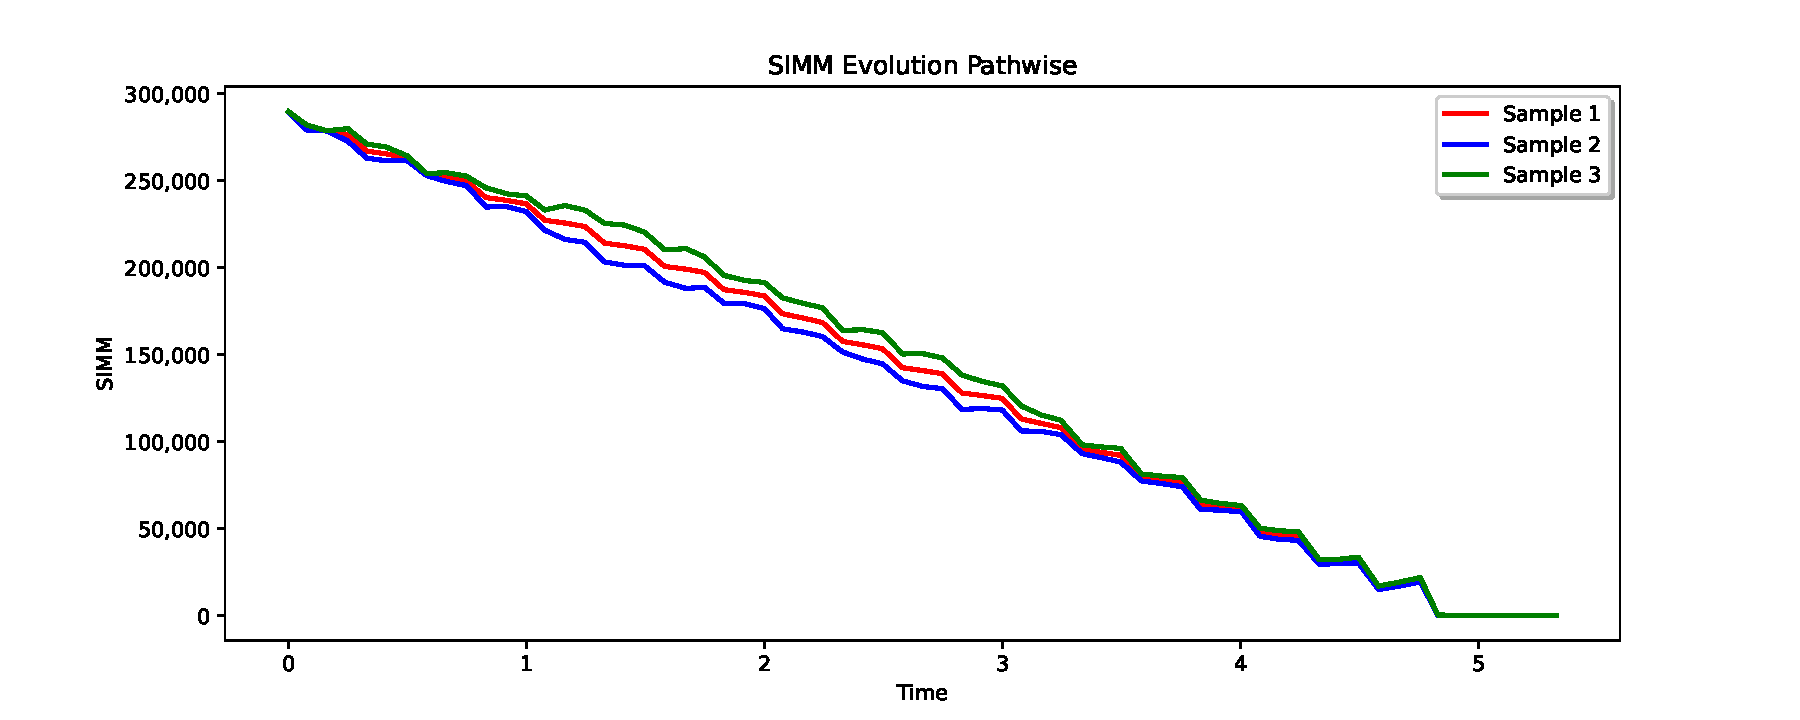
\includegraphics[width=0.8 \linewidth]{pics/fig_1_simm_evolution_pathwise_swap.pdf}}
\caption{Dynamic SIMM evolution along three representative Monte Carlo paths.}
\label{fig:swapevolution}
\end{figure}
In Figure \ref{fig:swapevolution_bench_1}, we compare one of these Dynamic SIMM paths (we have chosen sample \#3 arbitrarily here) to the benchmarks,
as well as against the simple regression model. The excellent match with the two benchmarks along the same market evolution is typical and can be
demonstrated similarly for other path choices.

\begin{figure}[h!]
\centering
%\fig{\includegraphics[width=0.8 \linewidth]{pics/mpl_simm_evolution_pathwise_1_0_swap.pdf}}
%\fig{\includegraphics[width=0.8 \linewidth]{pics/mpl_simm_evolution_pathwise_2_0_swap.pdf}}
\fig{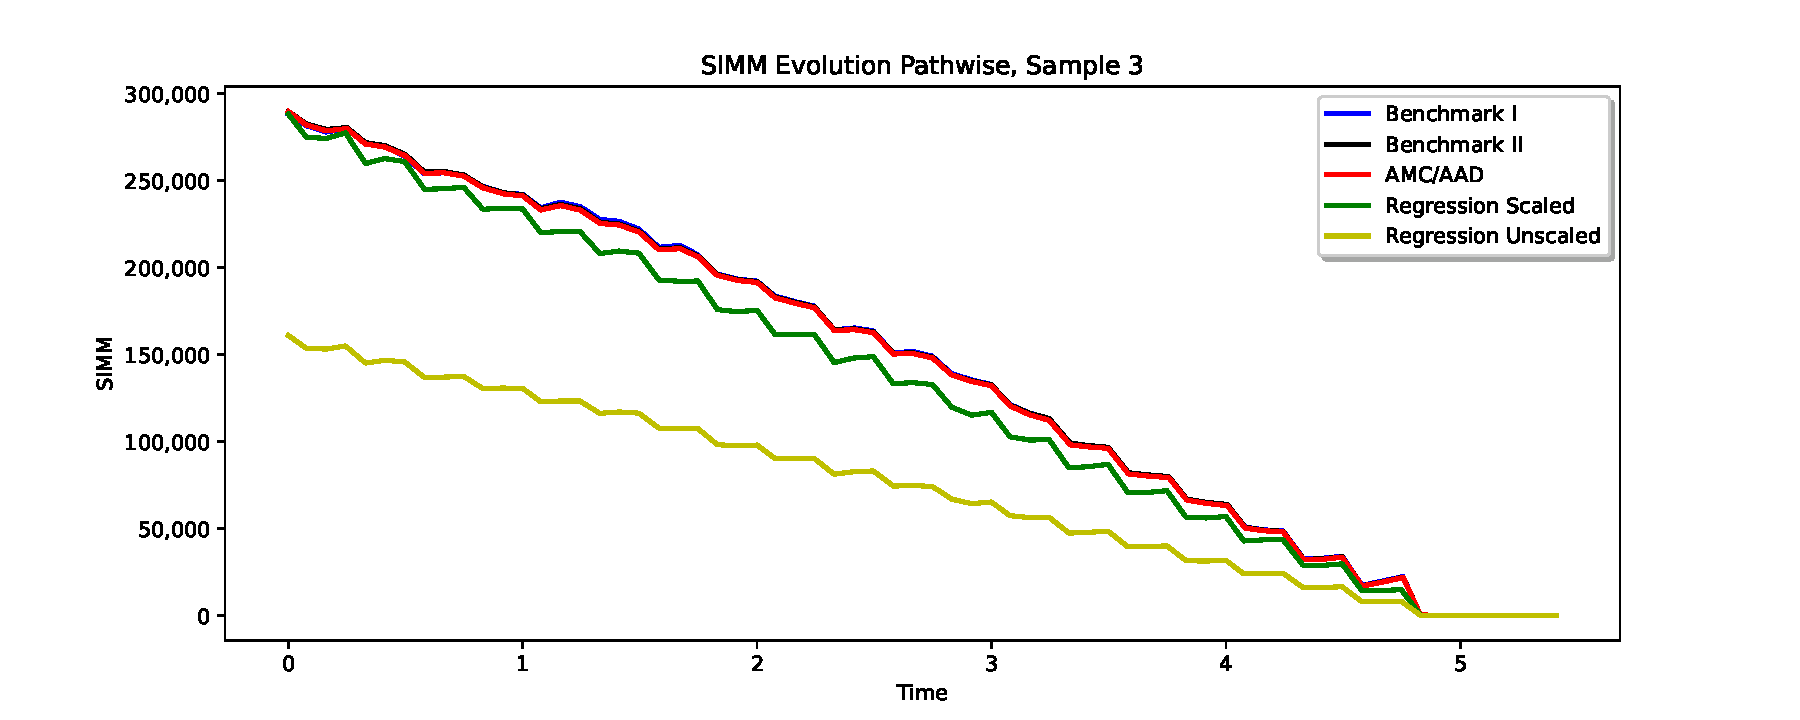
\includegraphics[width=0.8 \linewidth]{pics/fig_2_simm_evolution_pathwise_3_0_swap.pdf}}
\caption{Representative Dynamic SIMM path (red) -- compared to the simple regression model with and without $t_0$ scaling
  (dark and light green, respectively); the two benchmarks (blue and black) are again covered by the red Dynamic SIMM path with hardly
  noticeable deviations. }
\label{fig:swapevolution_bench_1}
\end{figure}
Obviously, the regression model requires scaling for a qualitative agreement with the Dynamic SIMM model or its benchmarks. The
reason is that the regression model's IM variance is based on the CAM calibration whereas ISDA SIMM has its own historical (and
stressed) calibration encoded in the SIMM risk weights. While the 75bp flat Swaption volatility used in the CAM calibration is
arbitrary, it is nevertheless inspired by realistic market levels on the valuation date, and the discrepancy observed in Figure
\ref{fig:swapevolution_bench_1} is not unusual.

In Figure \ref{fig:swapdistribution_benchmark} we show distributions of Dynamic SIMM (solid red histograms) at several selected points in time, compared to
Benchmark II distributions, and we observe a very close match.
\begin{figure}[h!]
\centering
\fig{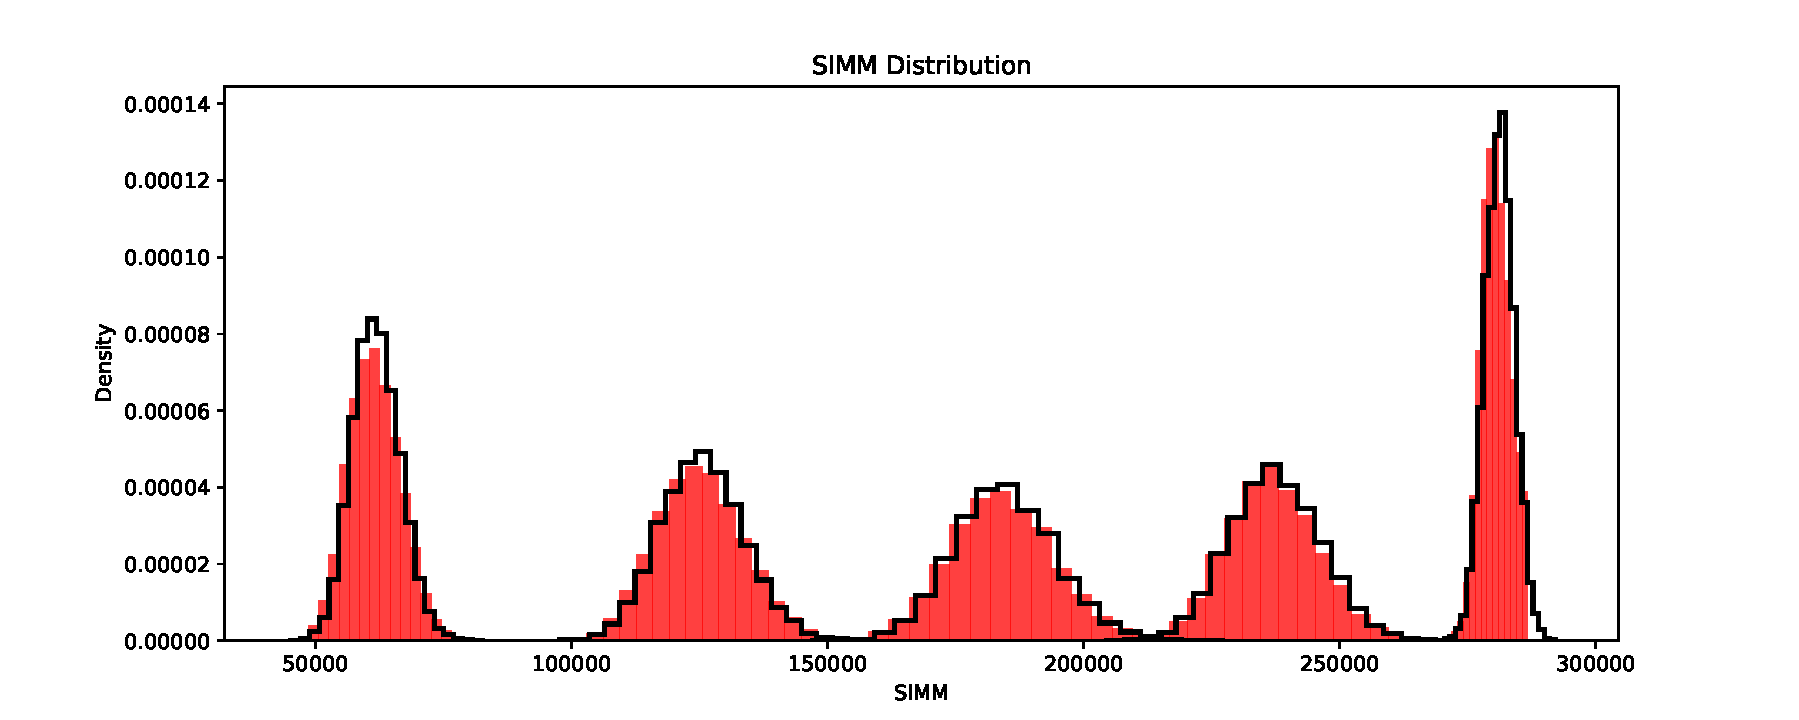
\includegraphics[width=0.8 \linewidth]{pics/fig_3_simm_distribution_swap_benchmark_2.pdf}}
\caption{Dynamic SIMM distribution at selected dates 1M, 1Y, 2Y, 3Y, 4Y in the future;
  the rightmost solid histogram (in red) is the Dynamic SIMM distribution associated with the 1M point, the leftmost point is associated with the 4Y point.
  The black solid line is the distribution generated by Benchmark II.
  Both Dynamic SIMM and Benchmark II distributions were compiled from 10,000 Monte Carlo paths.
}
\label{fig:swapdistribution_benchmark}
\end{figure}

\subsection{FX Forward}

To validate the Dynamic SIMM method for a basic linear FX product, we cover an FX Forward contract here, EUR/USD with maturity in 5Y and 1M
(matching the expiry of the FX Option in the following section \ref{sec:fxoption}). Figure \ref{fig:fxforwardevolution} shows the first three paths
as examples.
\begin{figure}[h!]
\centering
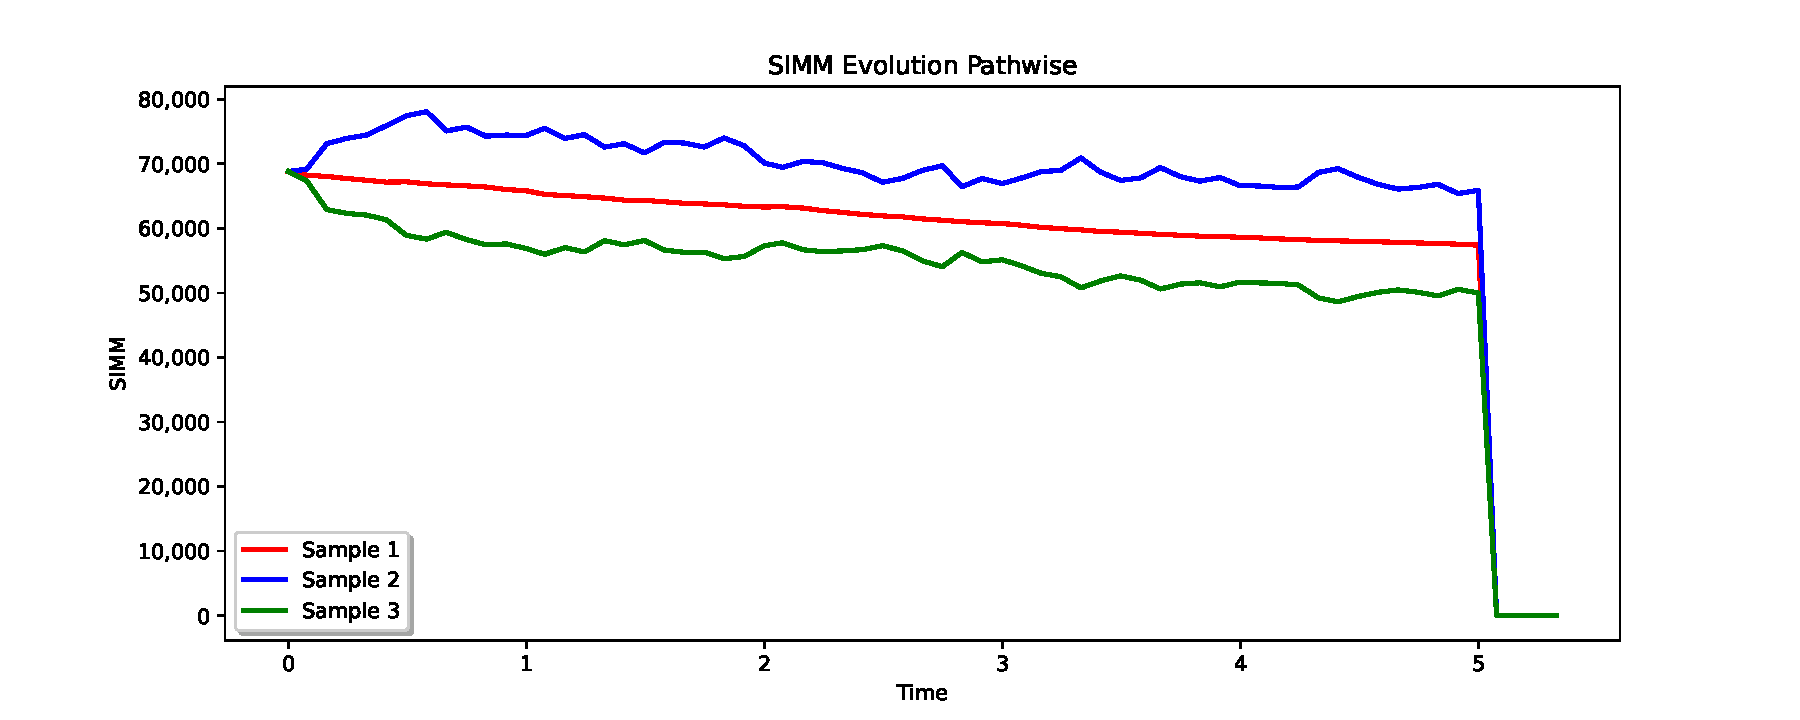
\includegraphics[width=1.0 \linewidth]{pics/mpl_simm_evolution_pathwise_fxforward.pdf}
\caption{Selected Dynamic SIMM paths for a EUR/USD FX Forward with maturity in 5Y and 1M.
  Note that path \#1 is particularly even because this is the first path from the Sobol Brownian Bridge generator used here.}
\label{fig:fxforwardevolution}
\end{figure}
For each of these paths see the benchmarking in figure \ref{fig:fxforwardevolution_bench}. Not only Dynamic SIMM model matches the benchmark here, even
the scaled simple regression model is fairly close in this particularly simple case.
\begin{figure}[h!]
\centering
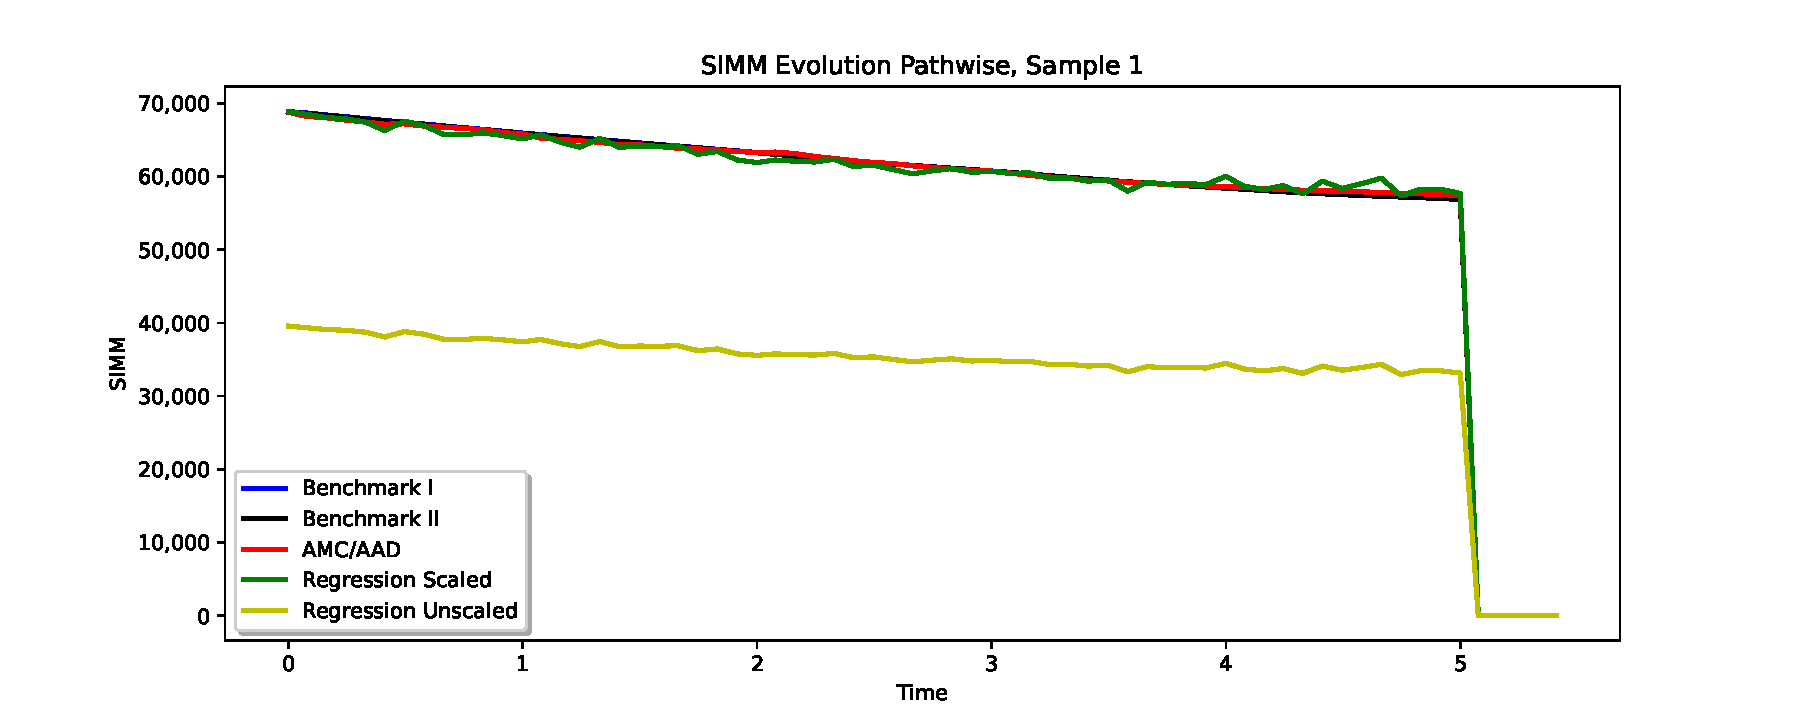
\includegraphics[width=1.0 \linewidth]{pics/mpl_simm_evolution_pathwise_1_0_fxforward.pdf}
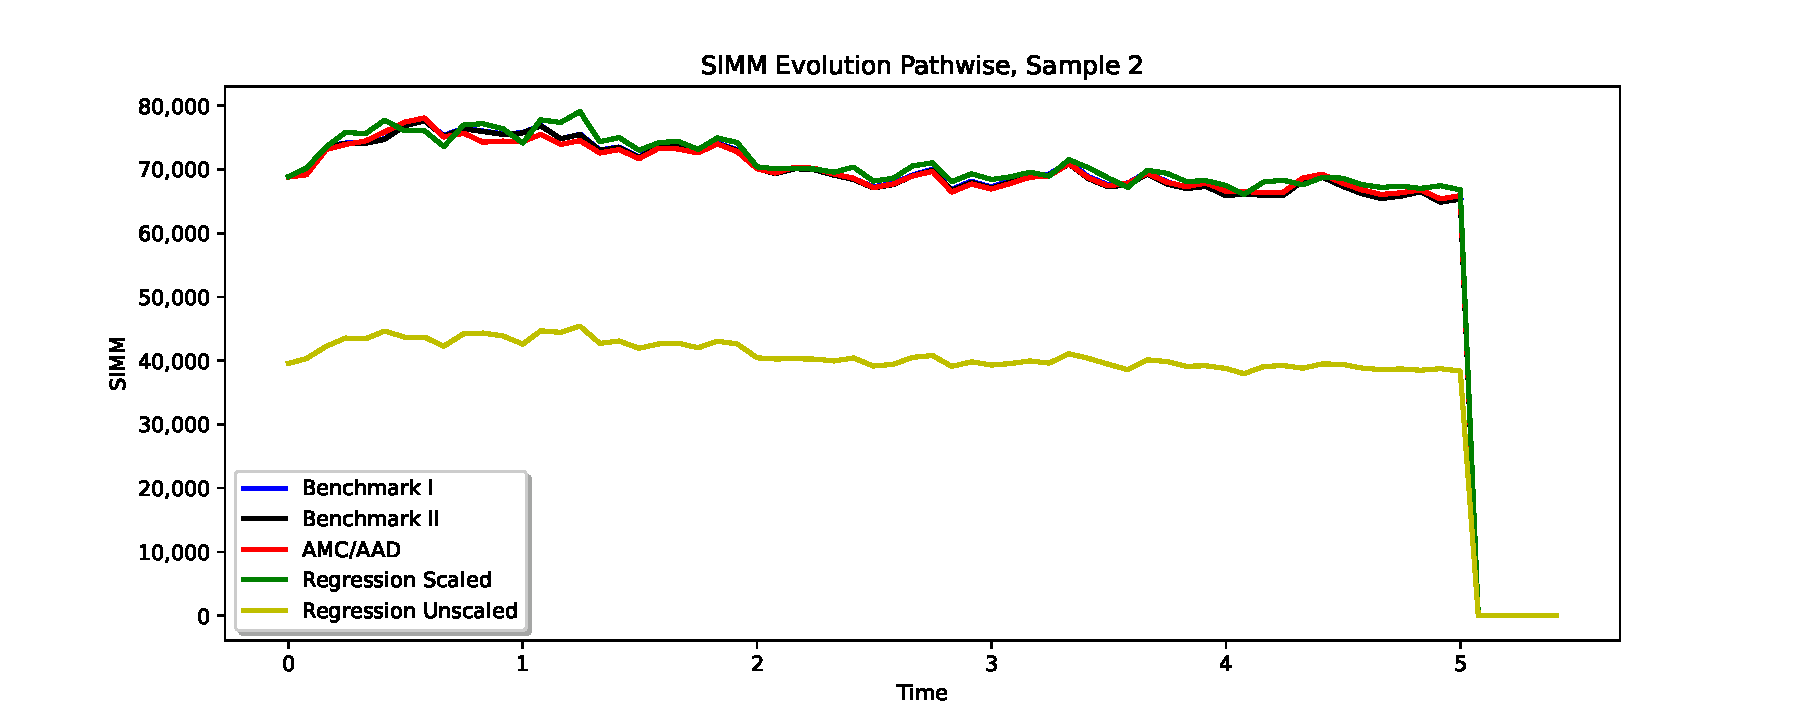
\includegraphics[width=1.0 \linewidth]{pics/mpl_simm_evolution_pathwise_2_0_fxforward.pdf}
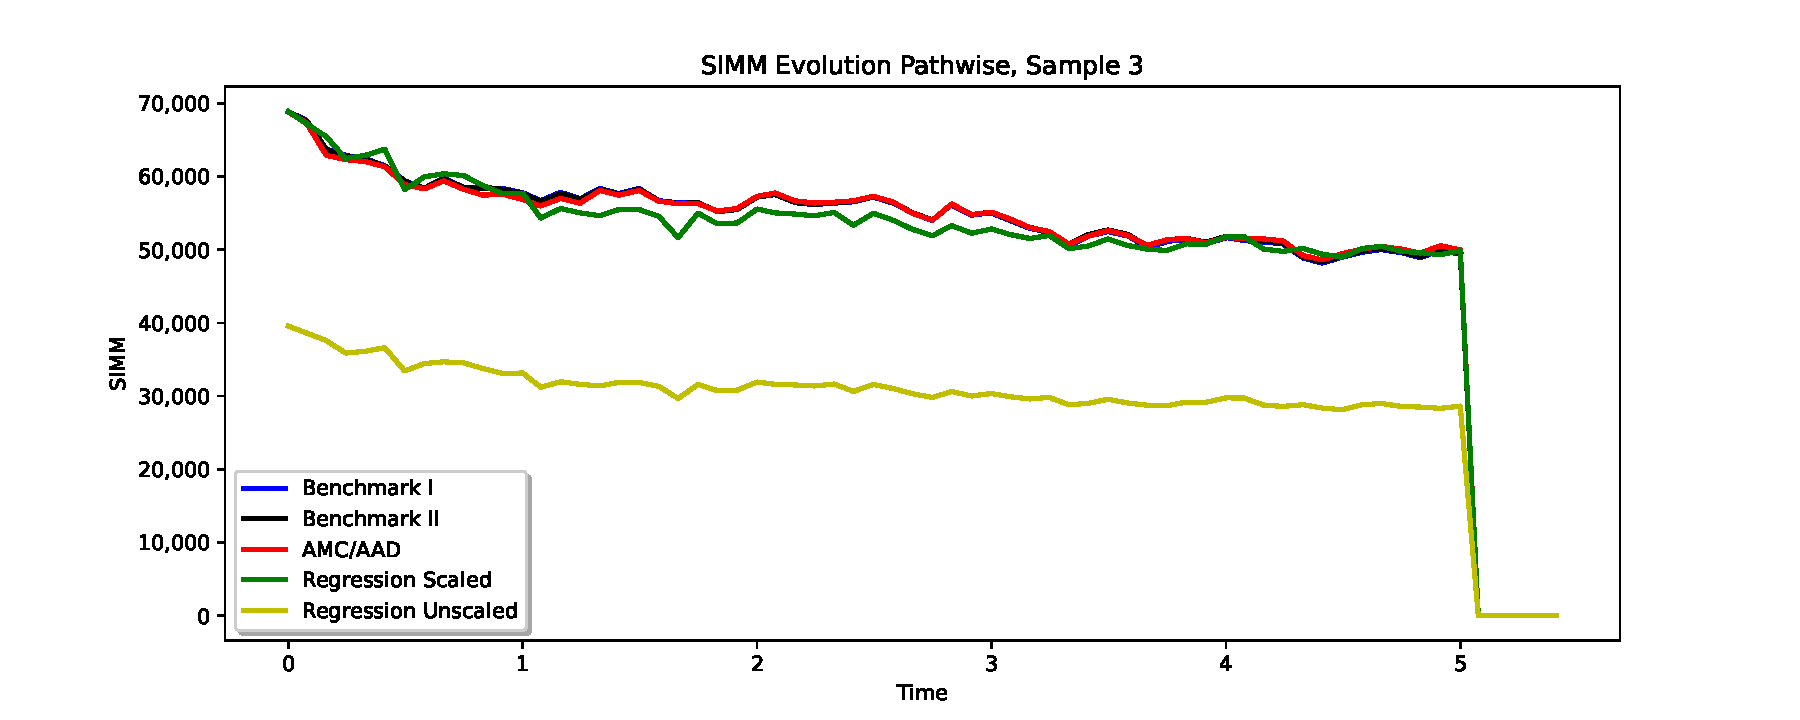
\includegraphics[width=1.0 \linewidth]{pics/mpl_simm_evolution_pathwise_3_0_fxforward.pdf}
\caption{FX Forward: Selected Dynamic SIMM path (red) vs benchmarks I and II (blue and black) and the simple regression model. }
\label{fig:fxforwardevolution_bench}
\end{figure}

\subsection{European FX Option}\label{sec:fxoption}

We now consider a Vanilla European EUR/USD FX Option with expiry in 5Y plus 1M.
Figure \ref{fig:fxoptionevolution} illustrates a few selected paths such that half of them end in the money and half out of the money.
\begin{figure}[h!]
\centering
\fig{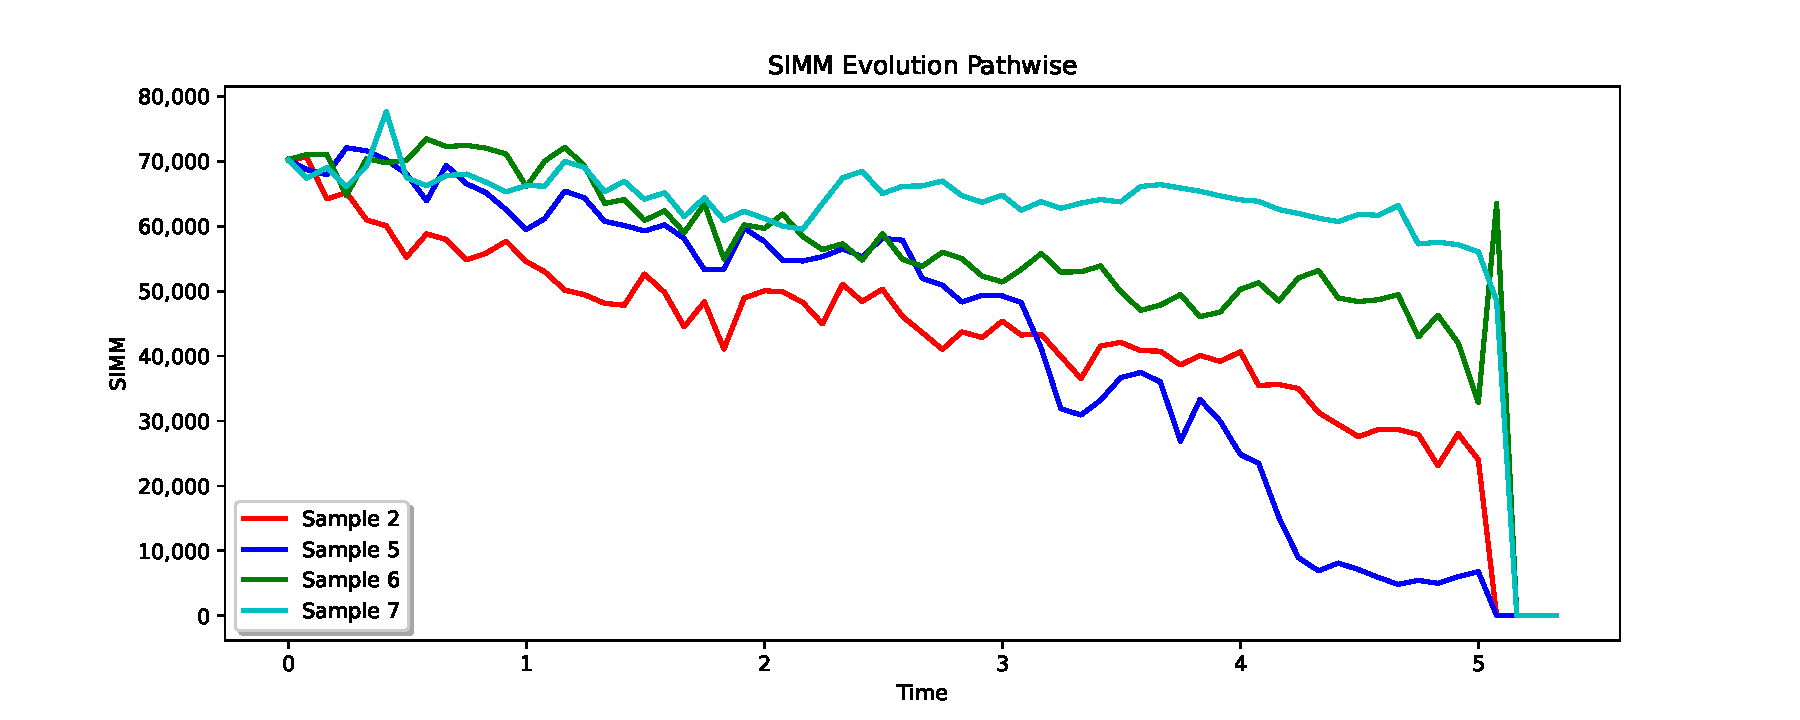
\includegraphics[width=0.8 \linewidth]{pics/fig_4_simm_evolution_pathwise_fxoption.pdf}}
\caption{FX Option: Selected Dynamic SIMM paths, two paths end out of the money (2 and 5), the others in the money.}
\label{fig:fxoptionevolution}
\end{figure}
In contrast to the previous section we first look at the benchmarking of {\em expected} SIMM evolution in Figure \ref{fig:fxoptionexpectedevolutionbench}.
\begin{figure}[h!]
\centering
\fig{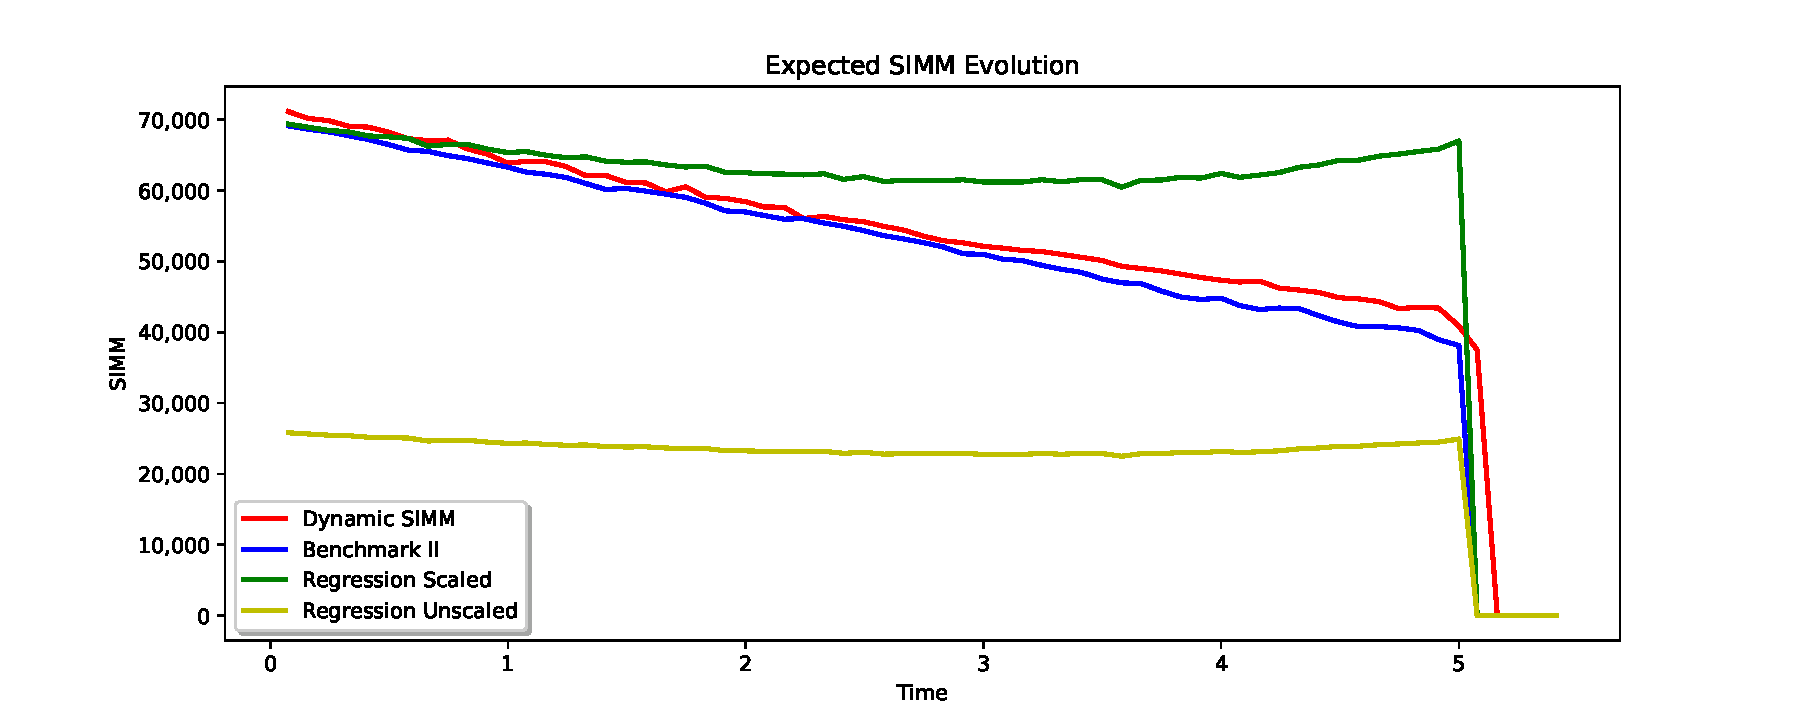
\includegraphics[width=0.8 \linewidth]{pics/fig_5_simm_evolution_expected_fxoption.pdf}}
\caption{FX Option: Expected SIMM evolution, Dynamic SIMM (10k paths) vs Benchmark II (100 paths) and Simple Regression (10k paths) paths. We skipped Benchmark I in
  this graph, because even 100 paths are computationally expensive with 60 monthly grid points. }
\label{fig:fxoptionexpectedevolutionbench}
\end{figure}
This shows clearly the deviation of the Simple Regression model from the benchmark (despite of $t_0$ scaling) as we approach option expiry.
This is the observation we made already in \cite{caspers2017_2} and one of the motivations to explore alternatives:
The Dynamic SIMM model stays much closer to the benchmark, although not as perfectly close as in the Swap case above. 
Figure \ref{fig:fxoptionpathwiseevolution_bench} then illustrates path-wise benchmark results for the same selected paths as shown in Figure
\ref{fig:fxoptionevolution}.
\begin{figure}[h!]
  \centering
  \begin{tabular}{cc}
\fig{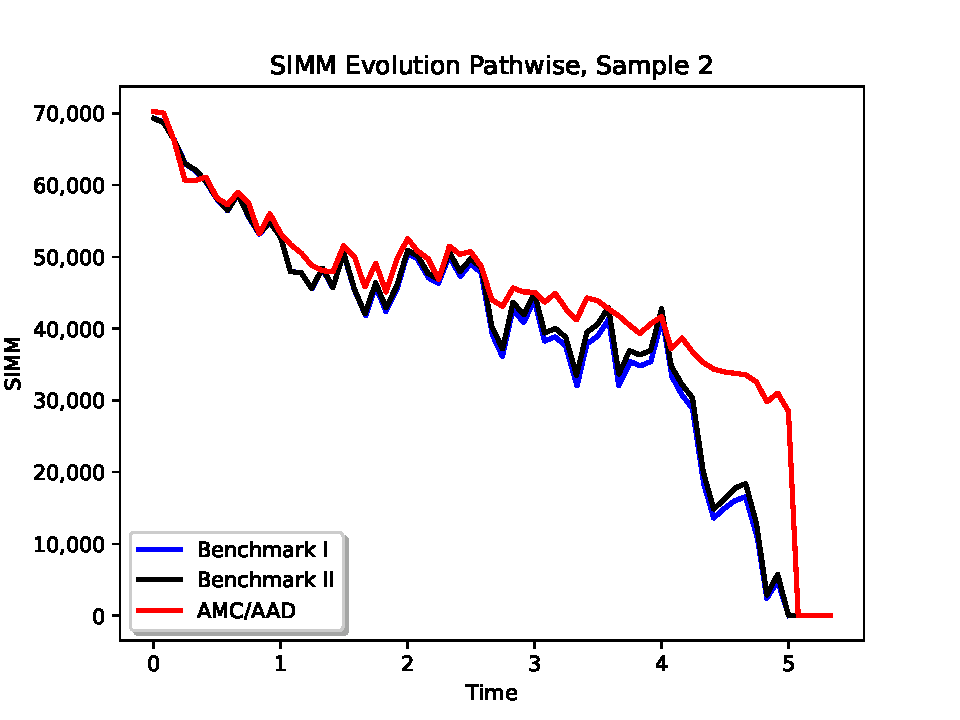
\includegraphics[width=0.5 \linewidth]{pics/fig_6a_simm_evolution_pathwise_2_0_fxoption_poly.pdf}} & 
\fig{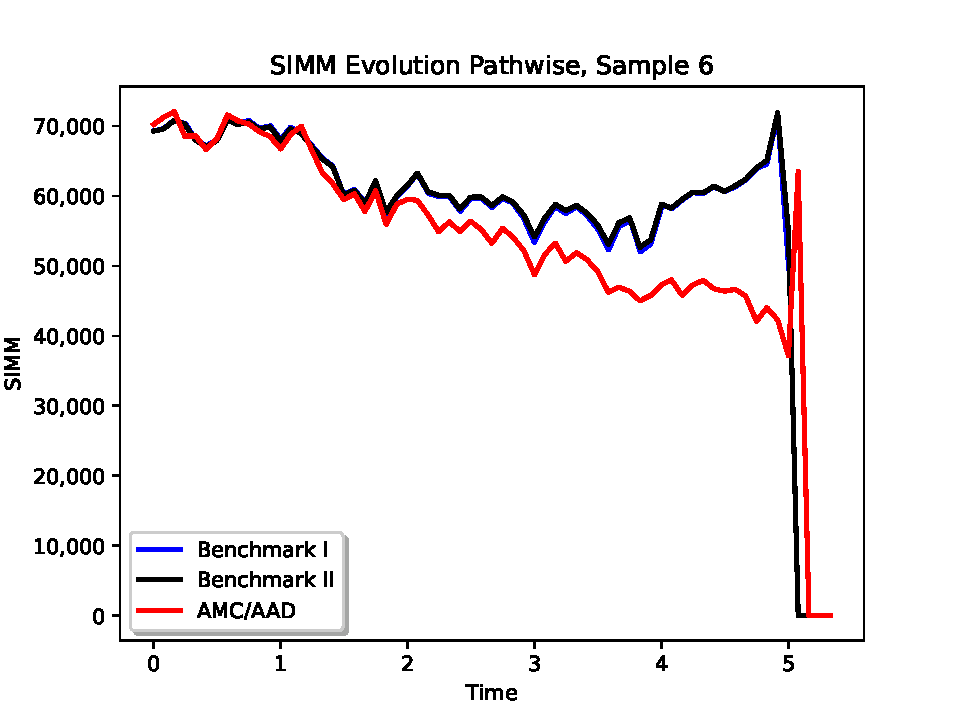
\includegraphics[width=0.5 \linewidth]{pics/fig_6b_simm_evolution_pathwise_6_0_fxoption_poly.pdf}} \\
\fig{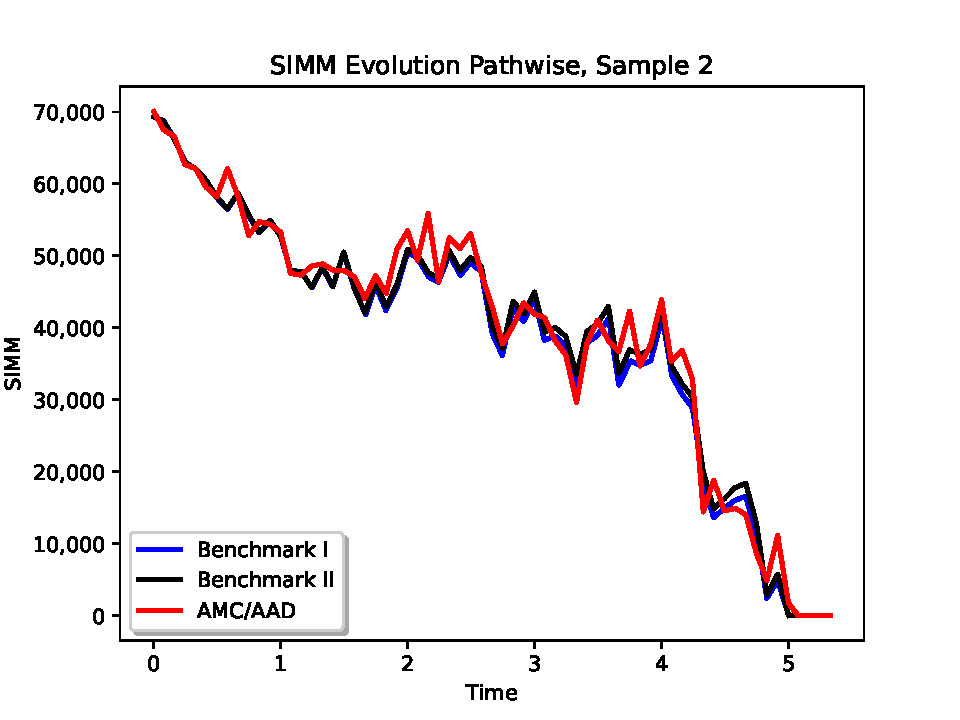
\includegraphics[width=0.5 \linewidth]{pics/fig_6c_simm_evolution_pathwise_2_0_fxoption_mars.pdf}} &
\fig{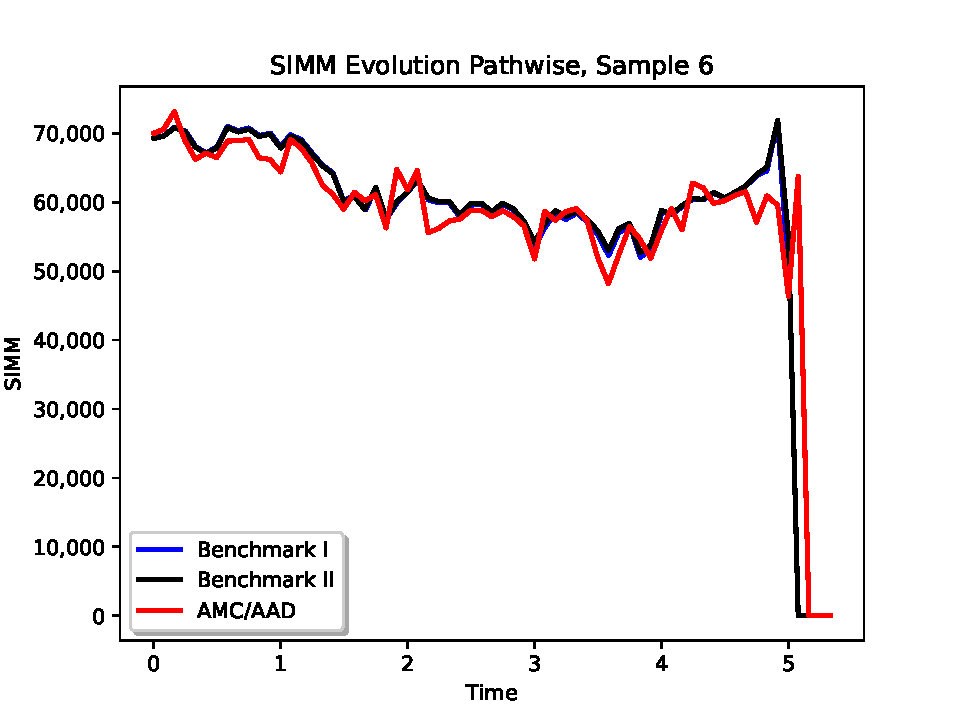
\includegraphics[width=0.5 \linewidth]{pics/fig_6d_simm_evolution_pathwise_6_0_fxoption_mars.pdf}}
\end{tabular}
  \caption{FX Option: Selected Dynamic SIMM path (red) vs benchmarks I and II (blue and black).
  Top: Polynomial regression order 4. Bottom: MARS regression (max terms 20), see below.}
\label{fig:fxoptionpathwiseevolution_bench}
\end{figure}

Focus on the top row in figure \ref{fig:fxoptionpathwiseevolution_bench} first: The individual paths are more ``bumpy'' than in the Swap case, and we see
small deviations although the Dynamic SIMM model tracks the benchmark paths overall. However, towards expiry we also see systematic deviations between Dynamic
SIMM model and Benchmark, more clearly on the individual paths than on average in
Figure \ref{fig:fxoptionexpectedevolutionbench}. Interestingly, we also see a slight discrepancy between our two benchmarks on the paths that end out
  of the money -- likely due to convexity effects (scaled partial derivatives vs large finite size bump shifts) or the fact we use a constant Jacobi matrix
  in Benchmark II -- however, the two benchmarks track each other very closely.
Figure \ref{fig:fxoptiondistribution4y} shows the Dynamic SIMM distribution at the 4Y point, i.e. 1Y before expiry.
\begin{figure}[h!]
\centering
\fig{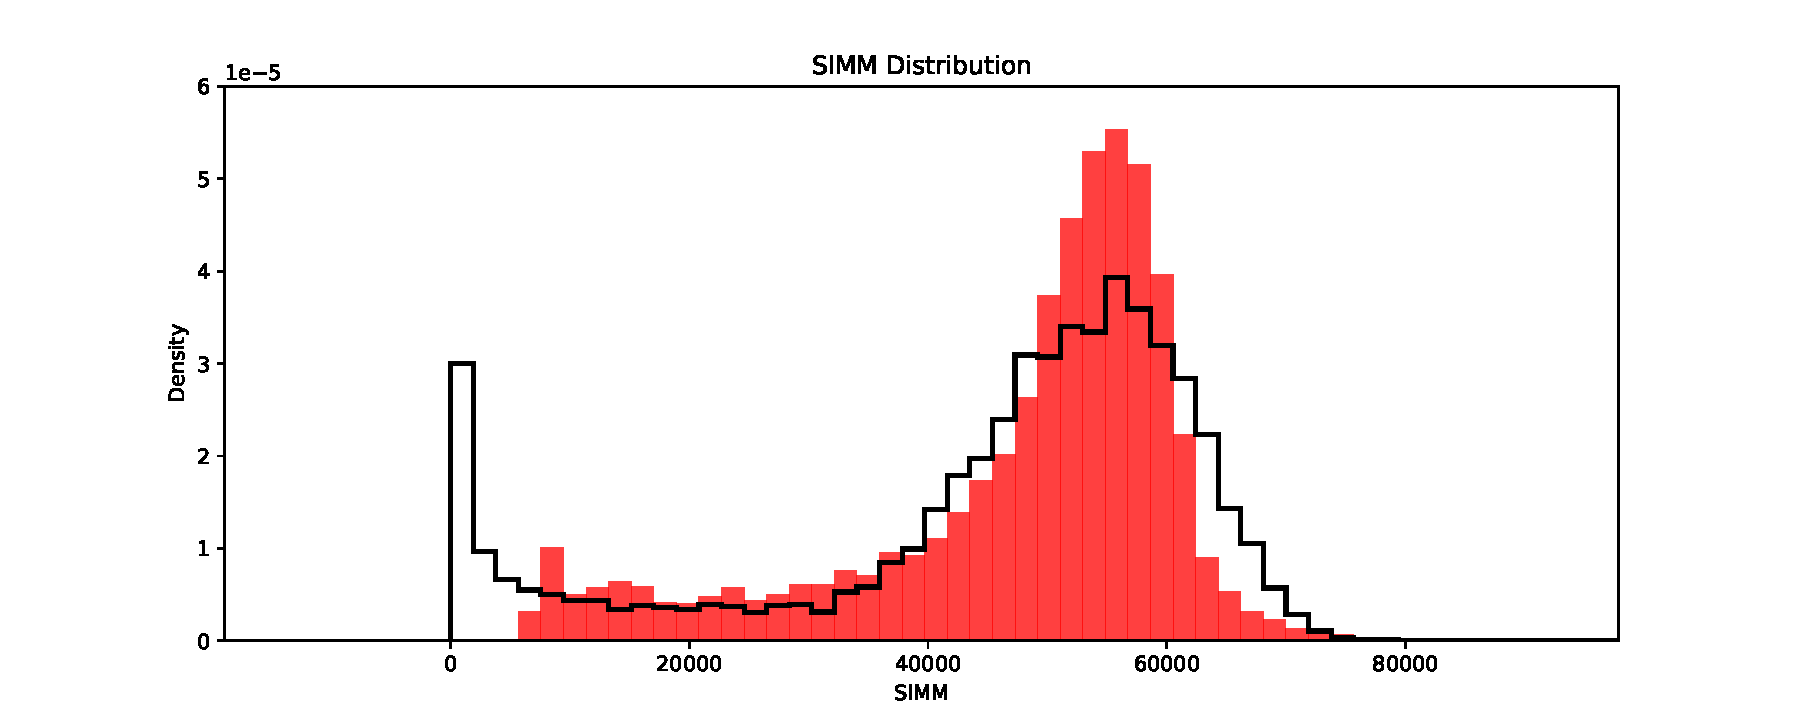
\includegraphics[width=0.8 \linewidth]{pics/fig_7a_simm_distribution_fxoption_4y_poly.pdf}}
\fig{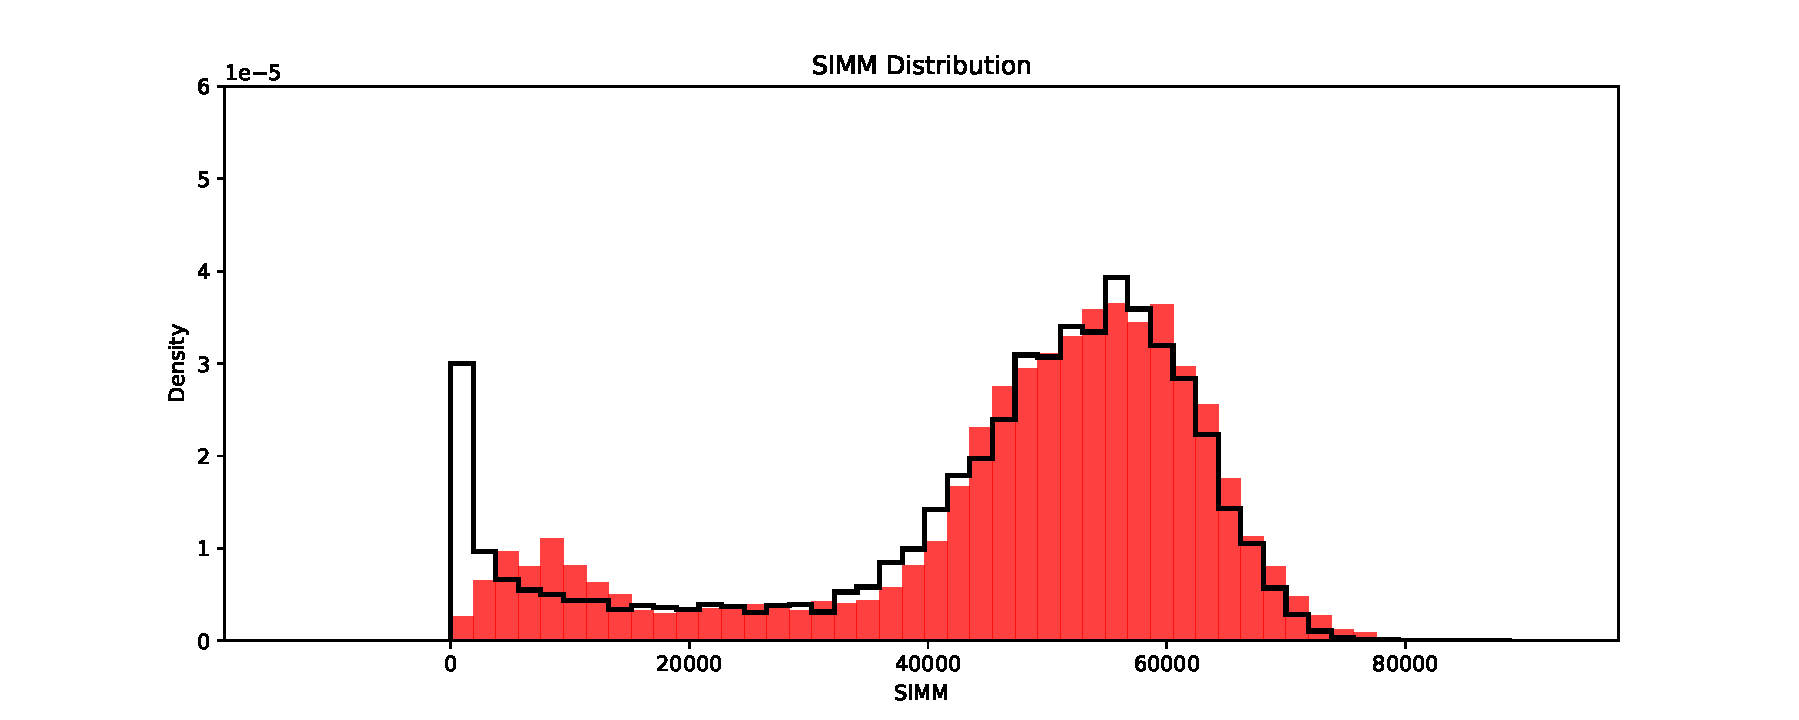
\includegraphics[width=0.8 \linewidth]{pics/fig_7b_simm_distribution_fxoption_4y_mars.pdf}}
\caption{FX Option: SIMM distribution at the 4y point, Dynamic SIMM (red, 10k paths) vs Benchmark II (black line, 100k paths). The Dynamic SIMM distribution was generated
  using AMC/AAD simulation with polynomial regression of order 4 (top) resp. with MARS regression, max degree 1, max terms 10 (bottom). }
\label{fig:fxoptiondistribution4y}
\end{figure}
This confirms the indication we got from individual paths (top row in figure \ref{fig:fxoptionexpectedevolutionbench}), there is a deviation close to expiry.
And the distribution view in figure \ref{fig:fxoptiondistribution4y} (top) shows that the model systematically underestimates the number / weights of paths that end up out of the money, where
the benchmark shows a pronounced peak at SIMM = 0.

We attribute the observed deviations to the regression method that we use within the AMC/AAD method of Dynamic SIMM up to this point (polynomial regression of order 4). 
When applied across the entire population of paths, those that are about to end in the money and those about to end out of the money,
this leads to a misrepresentation of the path-wise sensitivities and hence SIMM. The distribution view suggests that a {\em local} regression approach
might improve the match.

Following this idea we have explored several local, non-parametric me\-thods mentioned in section \ref{sec:sensi_regression}.
The bottom graph in figure \ref{fig:fxoptiondistribution4y} shows the Dynamic SIMM distribution at the 4Y point generated with MARS, which indicates
an improved match with the benchmark. The use of MARS also improves the path-wise benchmarking noticeably, as shown in the
bottom row of figure \ref{fig:fxoptionpathwiseevolution_bench}.

We can also measure the deviation using the root mean square error (RMSE) of the path-wise SIMM discrepancy
$$
\RMSE^2 = \frac{1}{N}\sum_{i=1}^N (\IM_{Model} - \IM_{Benchmark})^2
$$
In table \ref{tab:simm_error_fxoption} we
compare $\RMSE$ values for the FX Option case, across several regression models and at several points in time throughout the life of the
option. This confirms that the local regression methods appear to yield a better match with the benchmark closer to expiry, with
MARS consistently closest at the 3Y, 4Y and 5Y points, and similar to polynomial regression at the 1M, 1Y and 2Y points.
\begin{table}[hbt]
  \centering
  \begin{tabular}{|l|r|r|r|r|r|r|}
    \hline
    Regression Model         &  1M    & 1Y     & 2Y     & 3Y     & 4Y     & 5Y \\
    \hline
    \hline
    Polynomial               &  4,890 &  3,820 &  3,890 &  5,550 &  8,500 & 15,320 \\
    \hline 
    Regression Tree          & 10,810 & 10,150 & 10,000 & 10,400 &  8,100 & 10,940 \\
    \hline
    Nearest Neighbours        &  8,400 &  8,600 &  7,500 &  7,680 &  6,700 &  8,260  \\
    \hline
    MARS                     &  1,920 &  3,930 &  4,890 &  4,860 &  3,920 &  7,460 \\
    \hline
  \end{tabular}
  \caption{RMSE comparison across regression methods and at several selected points in time: Polynomial order 4, regression tree (depth 5), Nearest Neighbours (k=100), MARS. }
  \label{tab:simm_error_fxoption}
\end{table}

To illustrate the difference between the four regression methods in table \ref{tab:simm_error_fxoption}, we compare the
regression functions used to compute the FX Option's FX Delta at the 3y point. FX Delta is a dominant sensitivities that feeds into the
SIMM calculation, besides FX vega and IR Deltas in the respective currencies. Each sensitivity is modelled with a multi-variate
regression against three regressands here (the three relevant model states -- FX spot rate, LGM state variables in the two relevant
currencies). 
Orange points represent the regression model's FX Delta output, which is the conditional expectation of the regressand values (path-wise
FX Deltas), blue points. The orange model FX Delta curve is compared to the benchmark analytical
FX Deltas, green points.
\begin{figure}[h!]
\centering
\fig{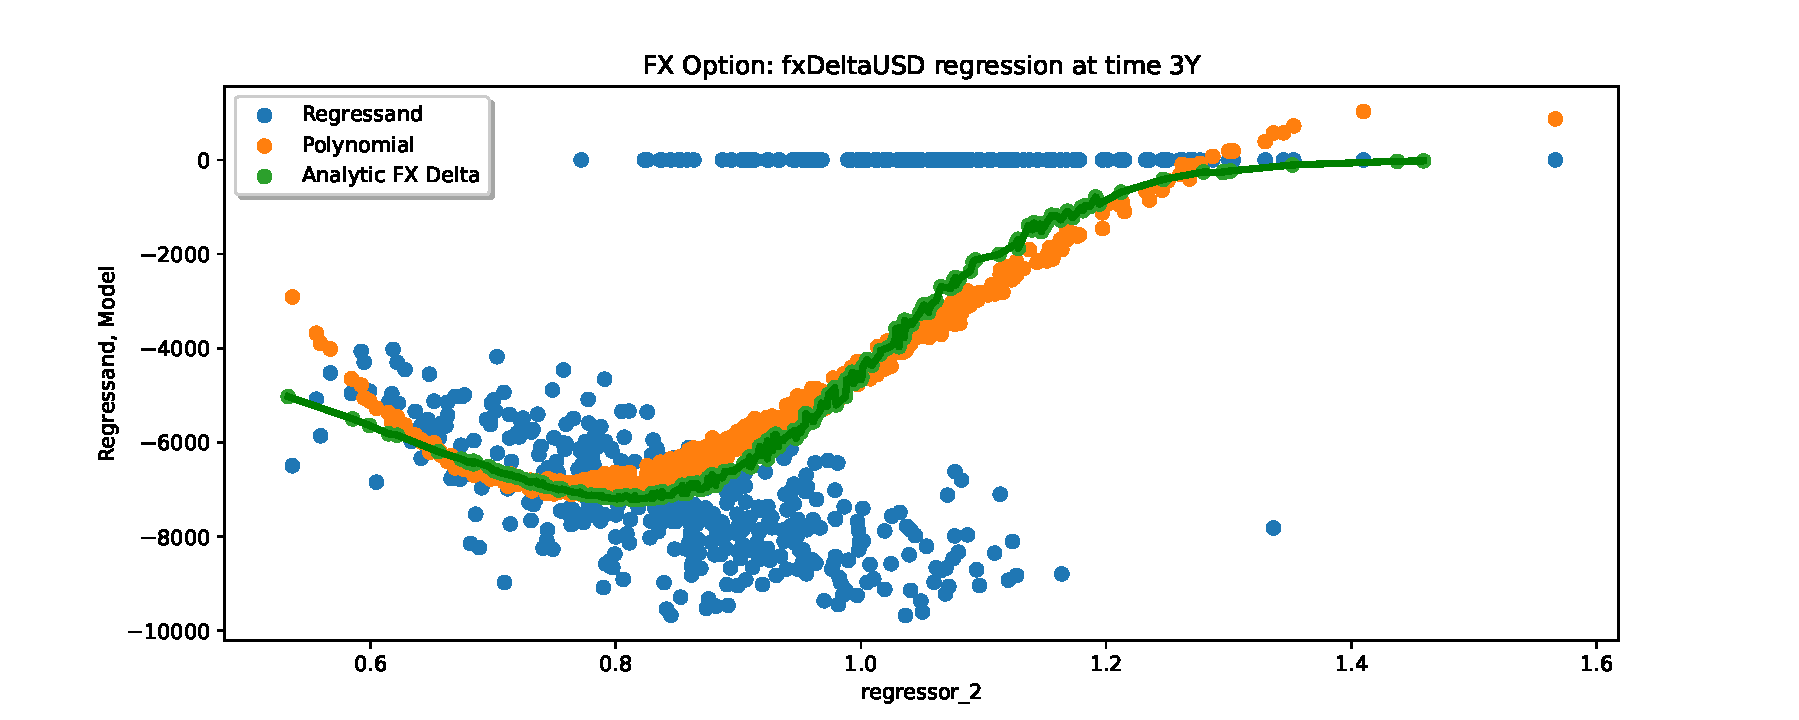
\includegraphics[width=0.8 \linewidth]{pics/fig_8a_regression_fxoption_poly_benchmark.pdf}}
\fig{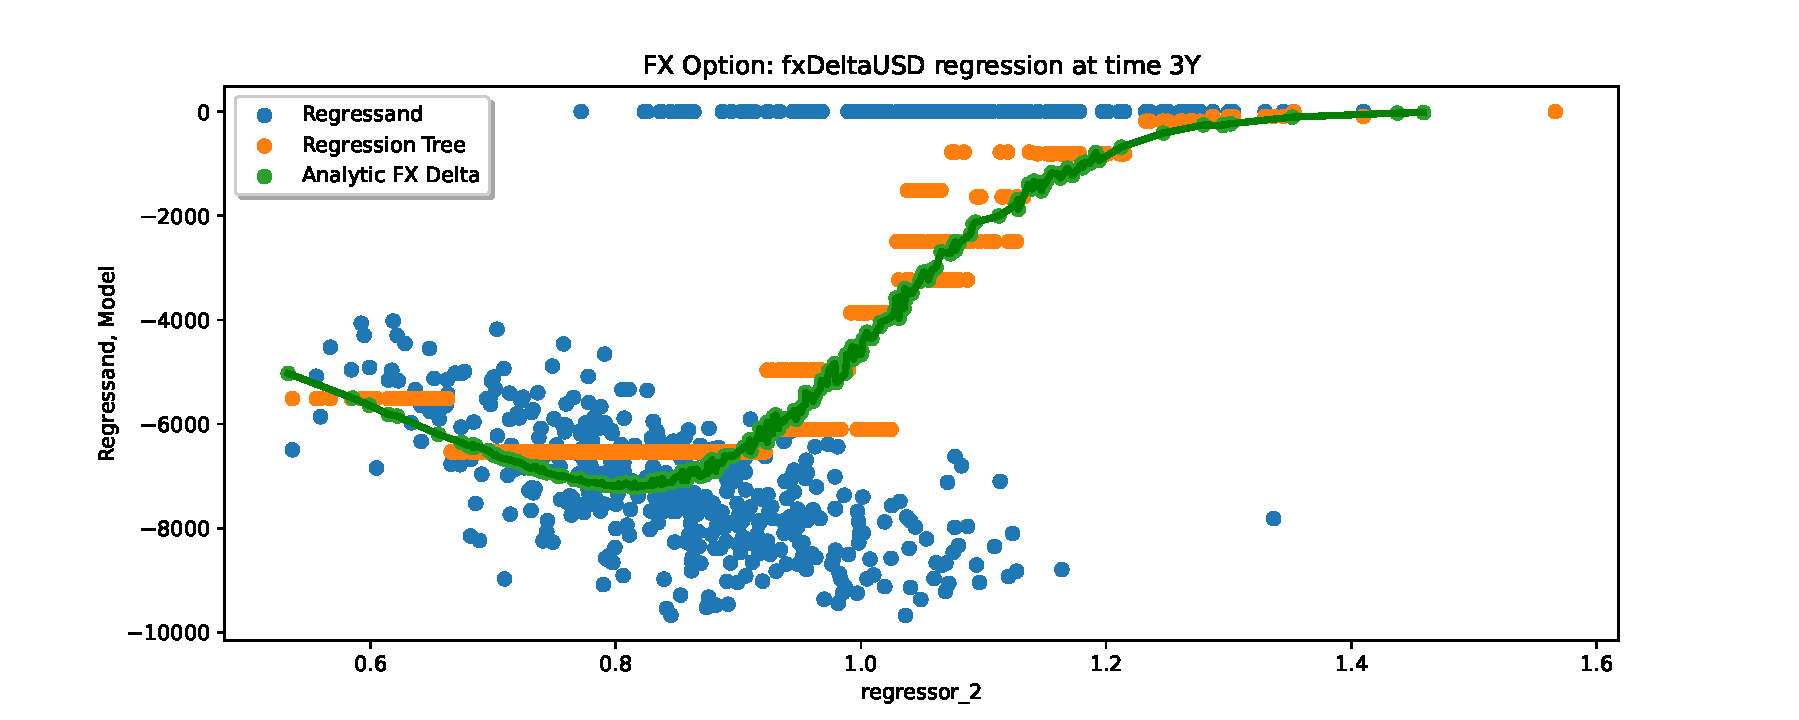
\includegraphics[width=0.8 \linewidth]{pics/fig_8b_regression_fxoption_tree_benchmark.pdf}}
\fig{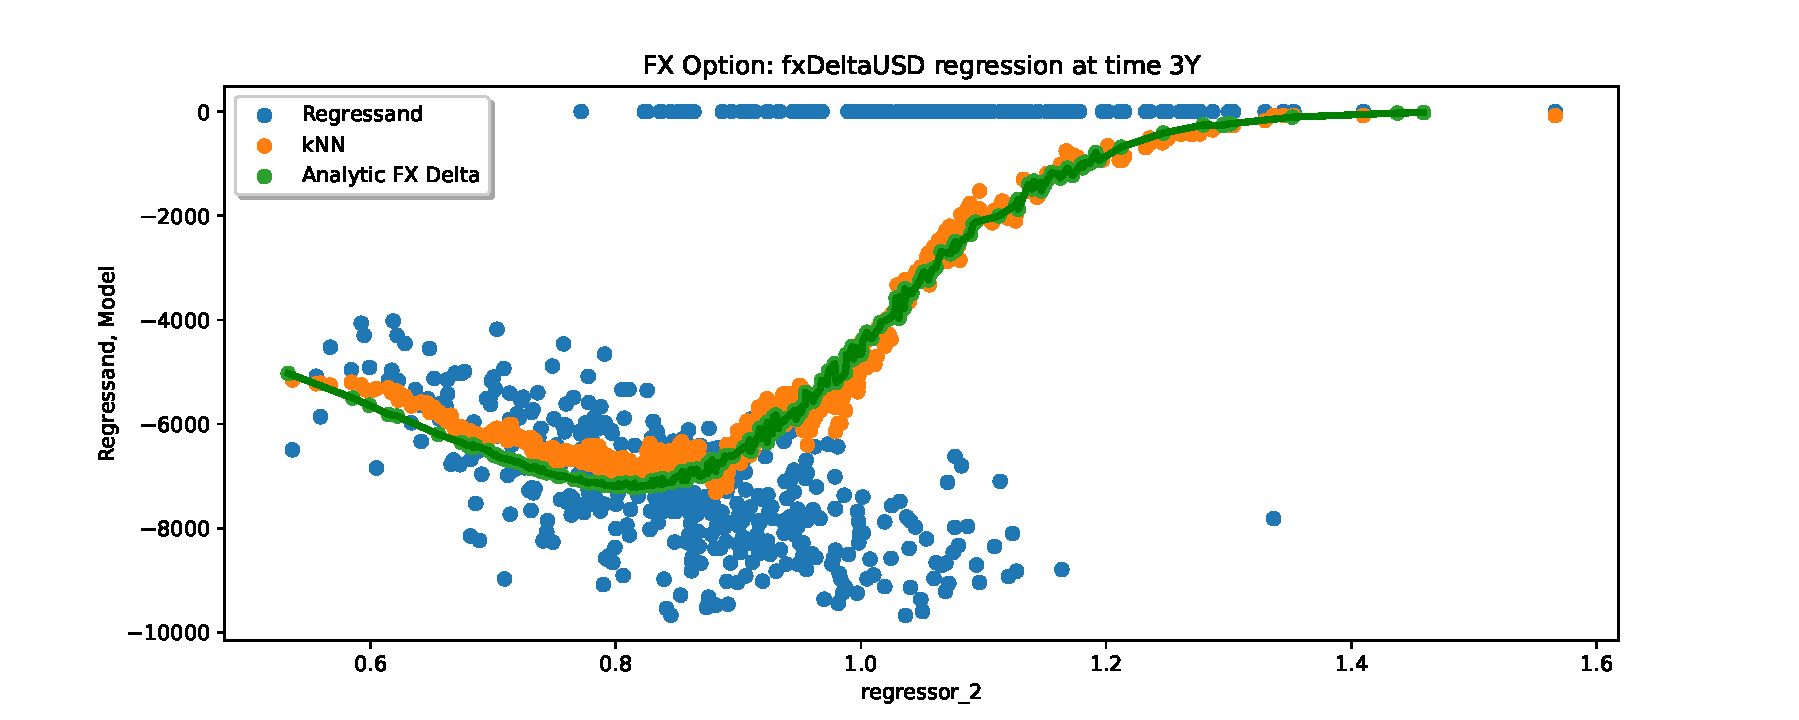
\includegraphics[width=0.8 \linewidth]{pics/fig_8c_regression_fxoption_knn100_benchmark.pdf}}
\fig{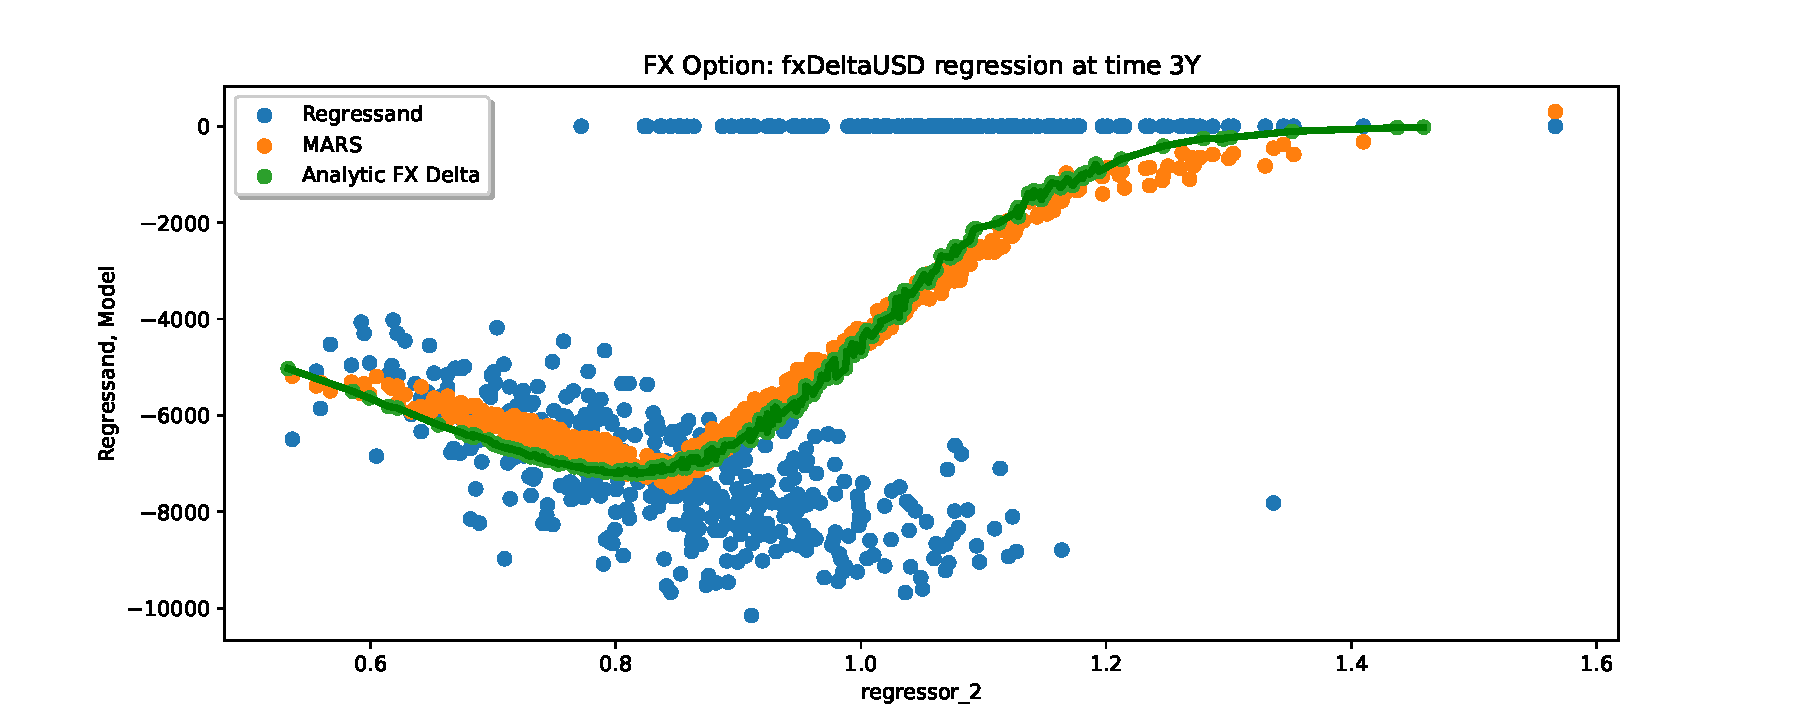
\includegraphics[width=0.8 \linewidth]{pics/fig_8d_regression_fxoption_mars_benchmark.pdf}}
\caption{FX Option: FX Delta regression at the 3y time point (orange), compared to benchmark FX Delta (green), for the four regression methods
  discussed in the text. To visualise the regression, we use the simulated data from a Dynamic SIMM run, regressand vs FX Spot regressor,
  filtering a narrow range ([-0.005,+0.005]) of the other two regressors (LGM state variables).}
\label{fig:fxoptionregression}
\end{figure}
The chain of blue points with Delta = 0 represents the paths that end out of the money, the blue cloud below represents paths that end in
the money. The conditional expectation averages across these outcomes, showing the signatures of the basis functions used, in particular the piecewise-linear
basis of the MARS method. Only kNN and MARS appear to reproduce the green benchmark Delta well in the middle of the regressor range.
Polynomial regression deviates from the benchmark across the range, in the middle of the data and in particular at the lower and upper ends of the regressor range.
The overall quality of the regression across all sensitivities is reflected at the SIMM level in the summary table \ref{tab:simm_error_fxoption}. 

To complete this FX Option study, we illustrate the striking mismatch of the scaled Simple Regression model resp. the significant improvement that the
Dynamic SIMM model offers, not only regarding SIMM average across paths, but also across the SIMM distribution.
\begin{figure}[h!]
\centering
\fig{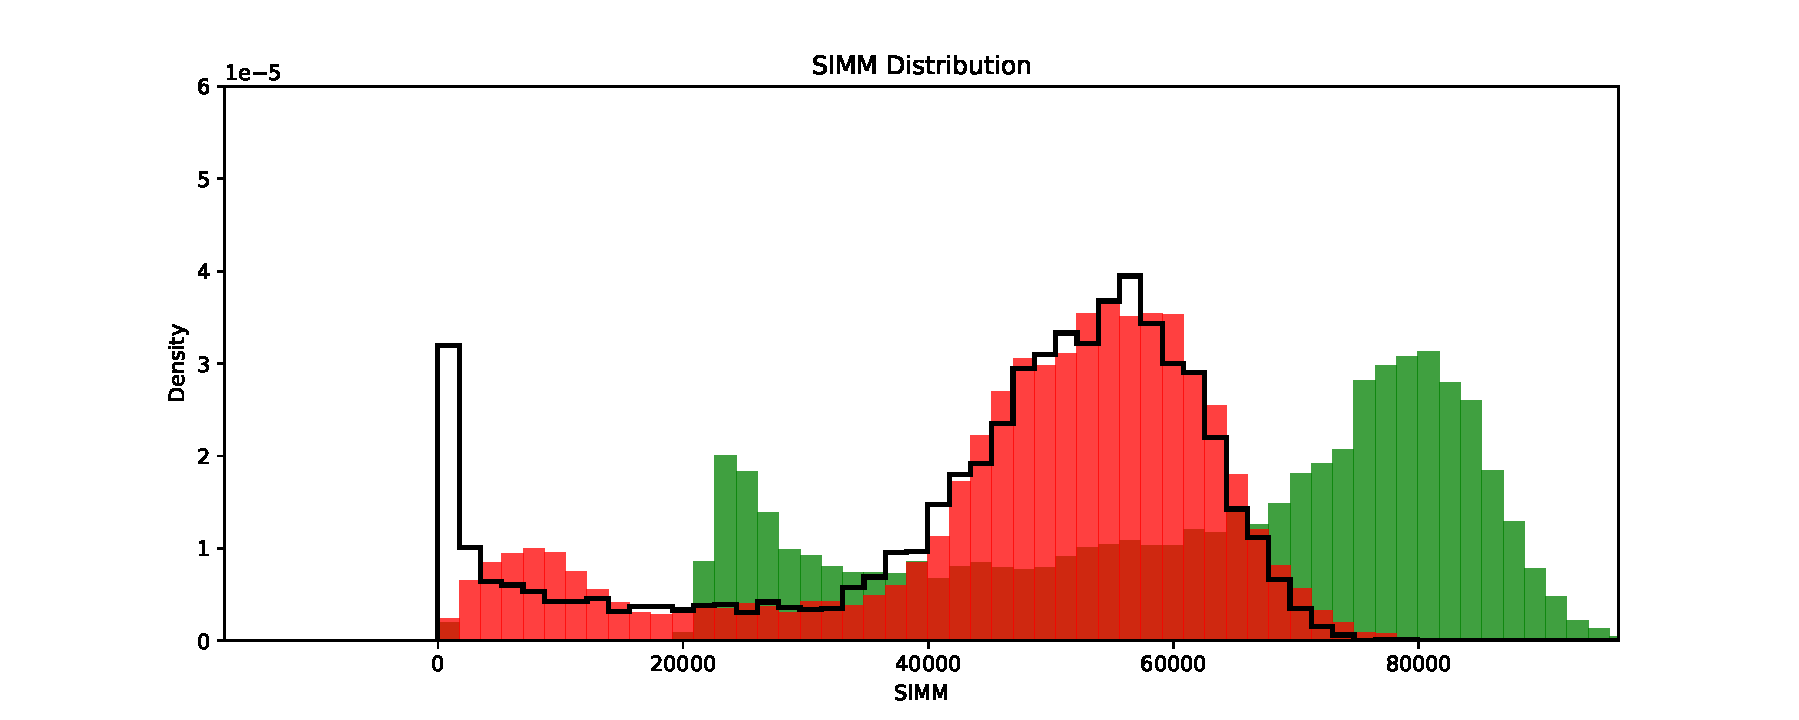
\includegraphics[width=1.0 \linewidth]{pics/fig_9_simm_distribution_fxoption_5y_mars_simple.pdf}}
\caption{FX Option: SIMM distribution 1M before expiry, Dynamic SIMM with MARS (red) vs Benchmark II (black line) and the scaled Simple Regression model (green). }
\label{fig:fxoptiondistribution5y_local_simple}
\end{figure}

\subsection{European Swaption}\label{sec:swaption}

In this section we briefly investigate the case of a Vanilla European Swaption in EUR, with expiry in 5Y and underlying Swap term 5Y, cash-settled, see
a few Dynamic SIMM model sample paths in figure \ref{fig:swaptionevolution}.
\begin{figure}[h!]
\centering
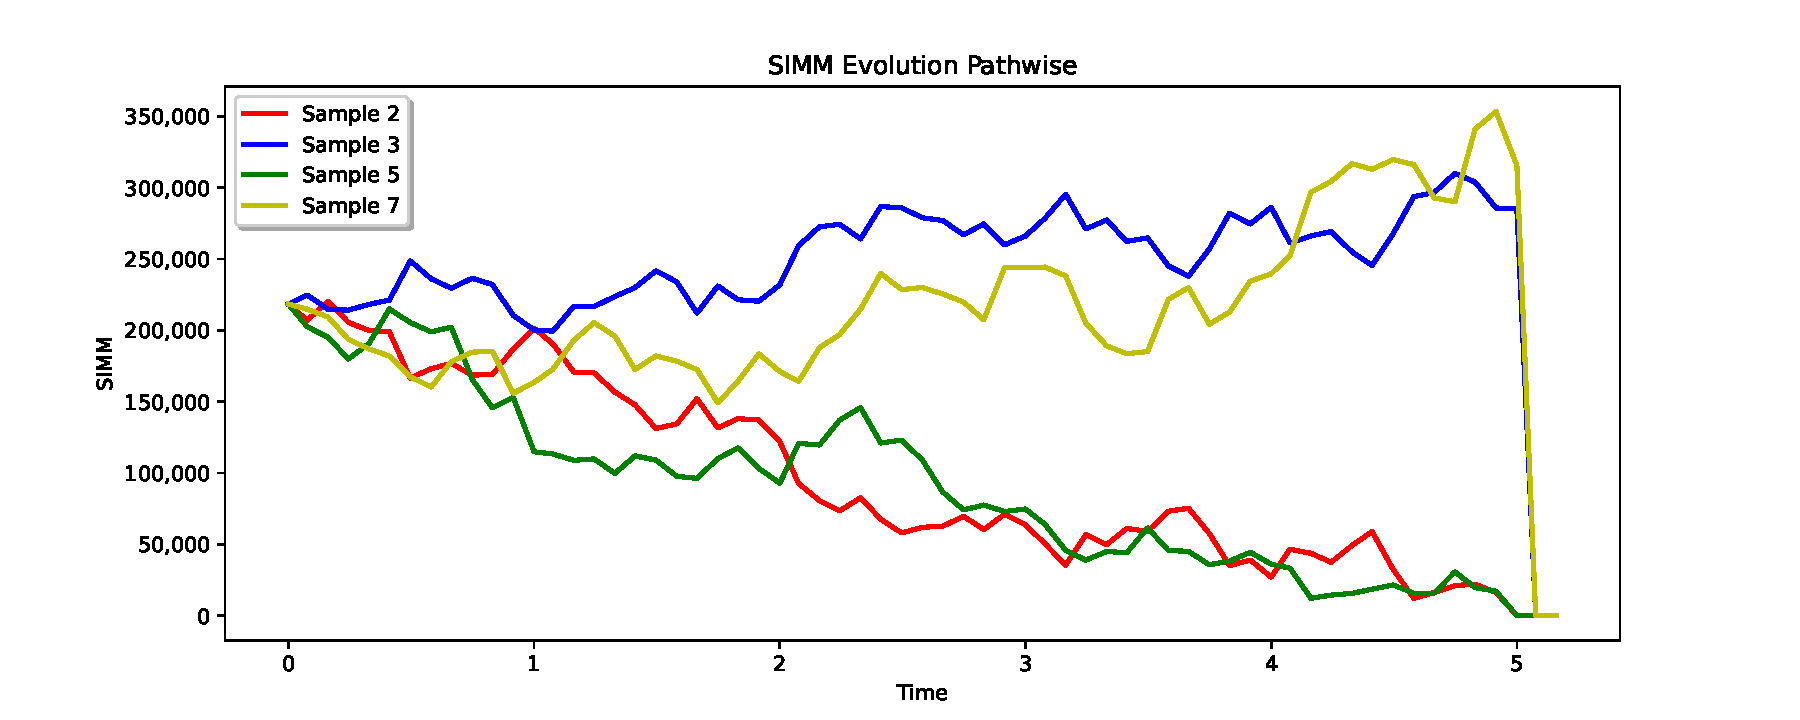
\includegraphics[width=1.0 \linewidth]{pics/mpl_simm_evolution_pathwise_swaption.pdf}
\caption{Swaption with expiry in 5Y: Selected Dynamic SIMM paths.}
\label{fig:swaptionevolution}
\end{figure}
The pathwise comparison to benchmarks in figure \ref{fig:swaptionevolution_bench} shows a similar match as in the FX Option case above. 
\begin{figure}[h!]
\centering
  \begin{tabular}{cc}
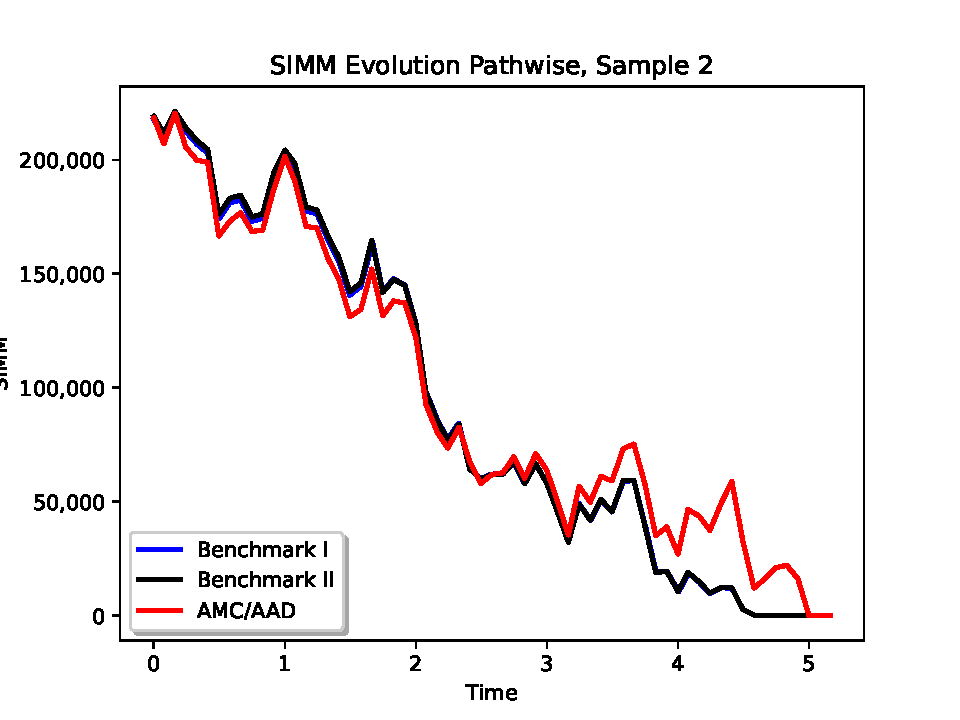
\includegraphics[width=0.5 \linewidth]{pics/mpl_simm_evolution_pathwise_2_0_swaption_poly.pdf} &
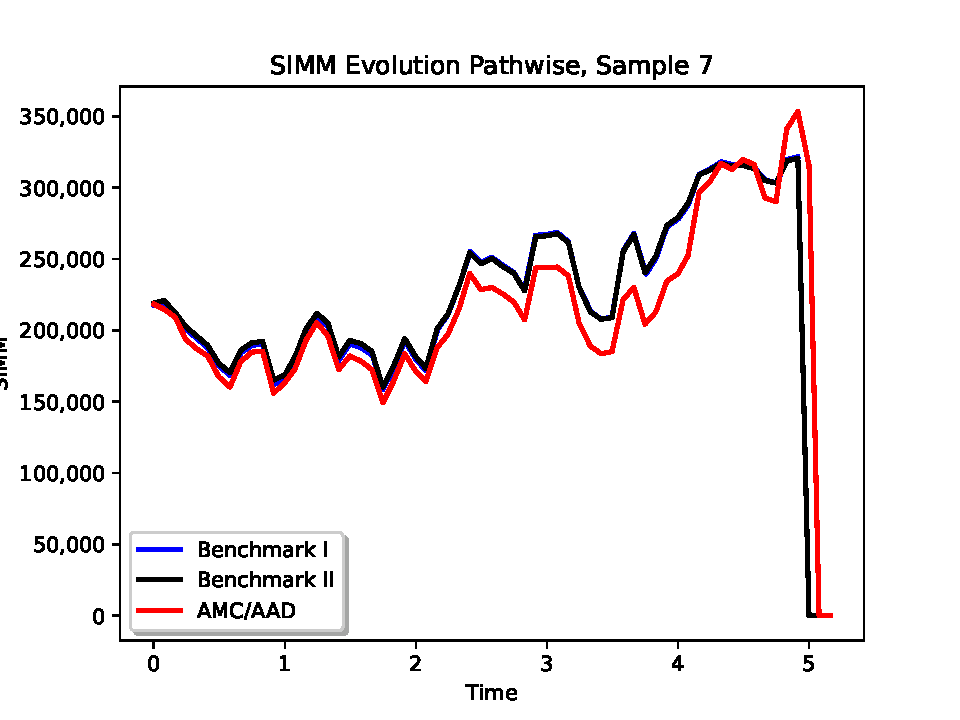
\includegraphics[width=0.5 \linewidth]{pics/mpl_simm_evolution_pathwise_7_0_swaption_poly.pdf} \\
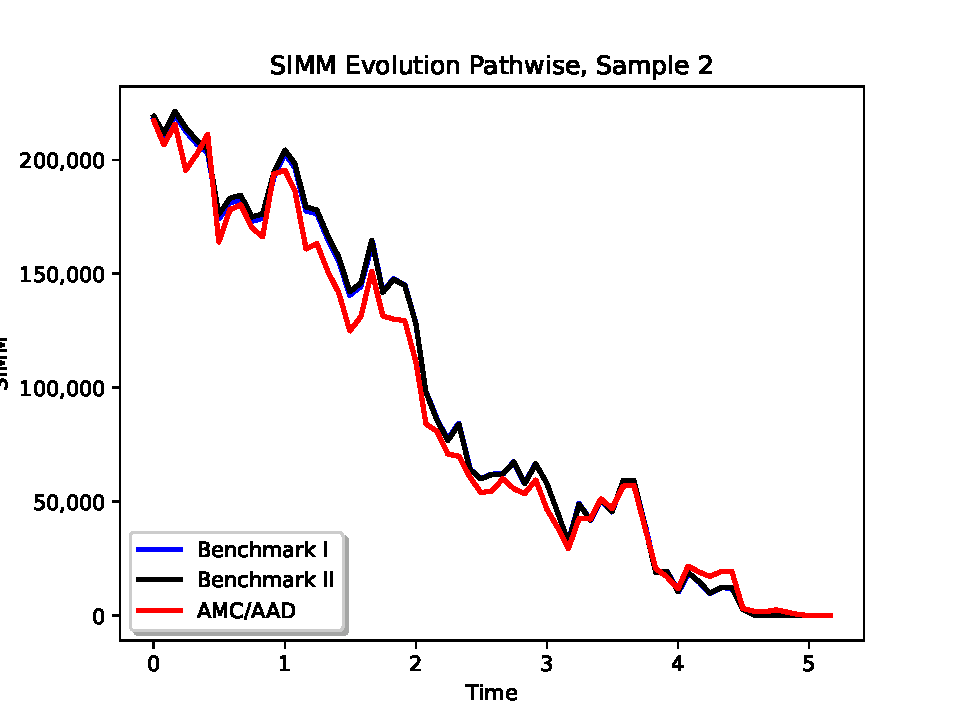
\includegraphics[width=0.5 \linewidth]{pics/mpl_simm_evolution_pathwise_2_0_swaption_mars.pdf} &
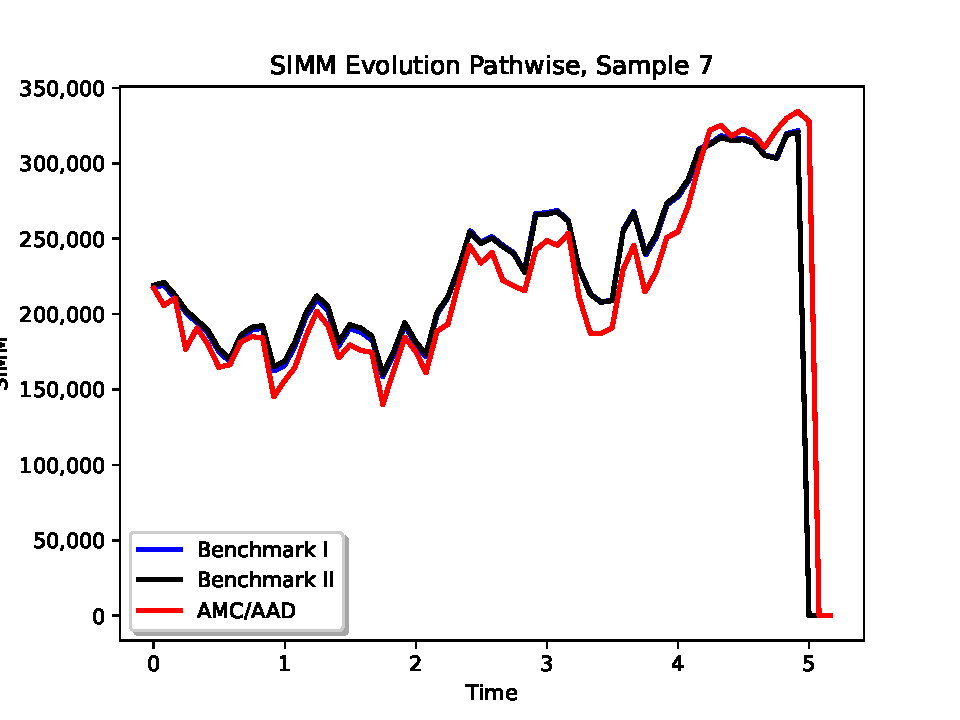
\includegraphics[width=0.5 \linewidth]{pics/mpl_simm_evolution_pathwise_7_0_swaption_mars.pdf} \\
  \end{tabular}
  \caption{European Swaption: Selected Dynamic SIMM path (red) vs benchmarks I and II (blue and black).
  Top: Dynamic SIMM with polyomial regression order 4.
  Bottom: Dynamic SIMM with MARS (max terms 20) regression improves the match on sample 2 towards expiry. }
\label{fig:swaptionevolution_bench}
\end{figure}
Overall, the Dynamic SIMM model tracks the benchmark well along the paths, with the notable exception of times close to expiry, and especially when paths run out
of the money. This is improved by local regression, see figure \ref{fig:swaptiondistribution_bench} for the distribution view shortly before expiry.
\begin{figure}[h!]
\centering
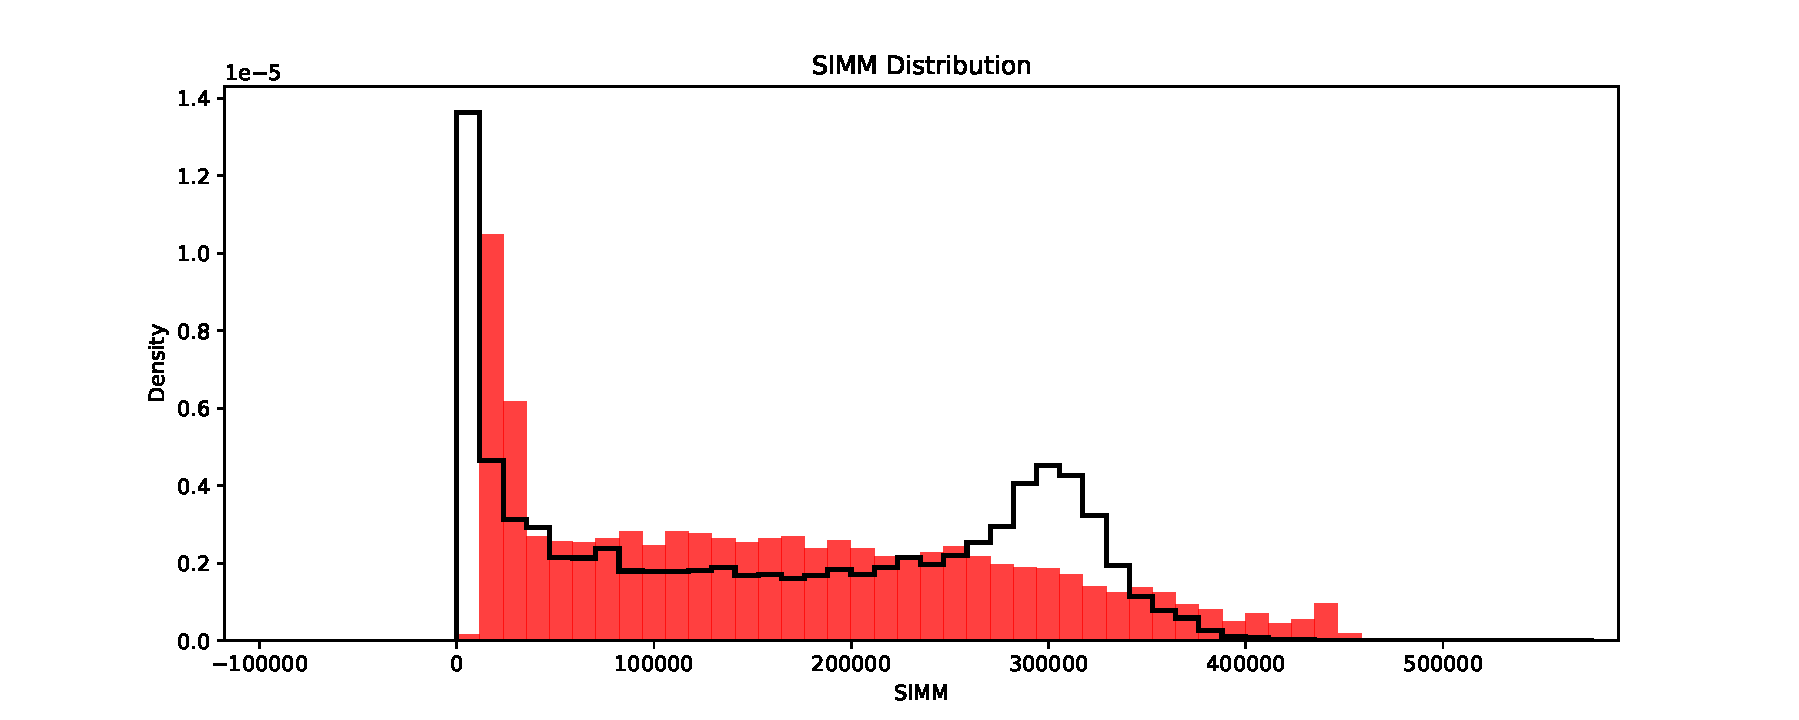
\includegraphics[width=1.0 \linewidth]{pics/mpl_simm_distribution_swaption_5y_poly.pdf}
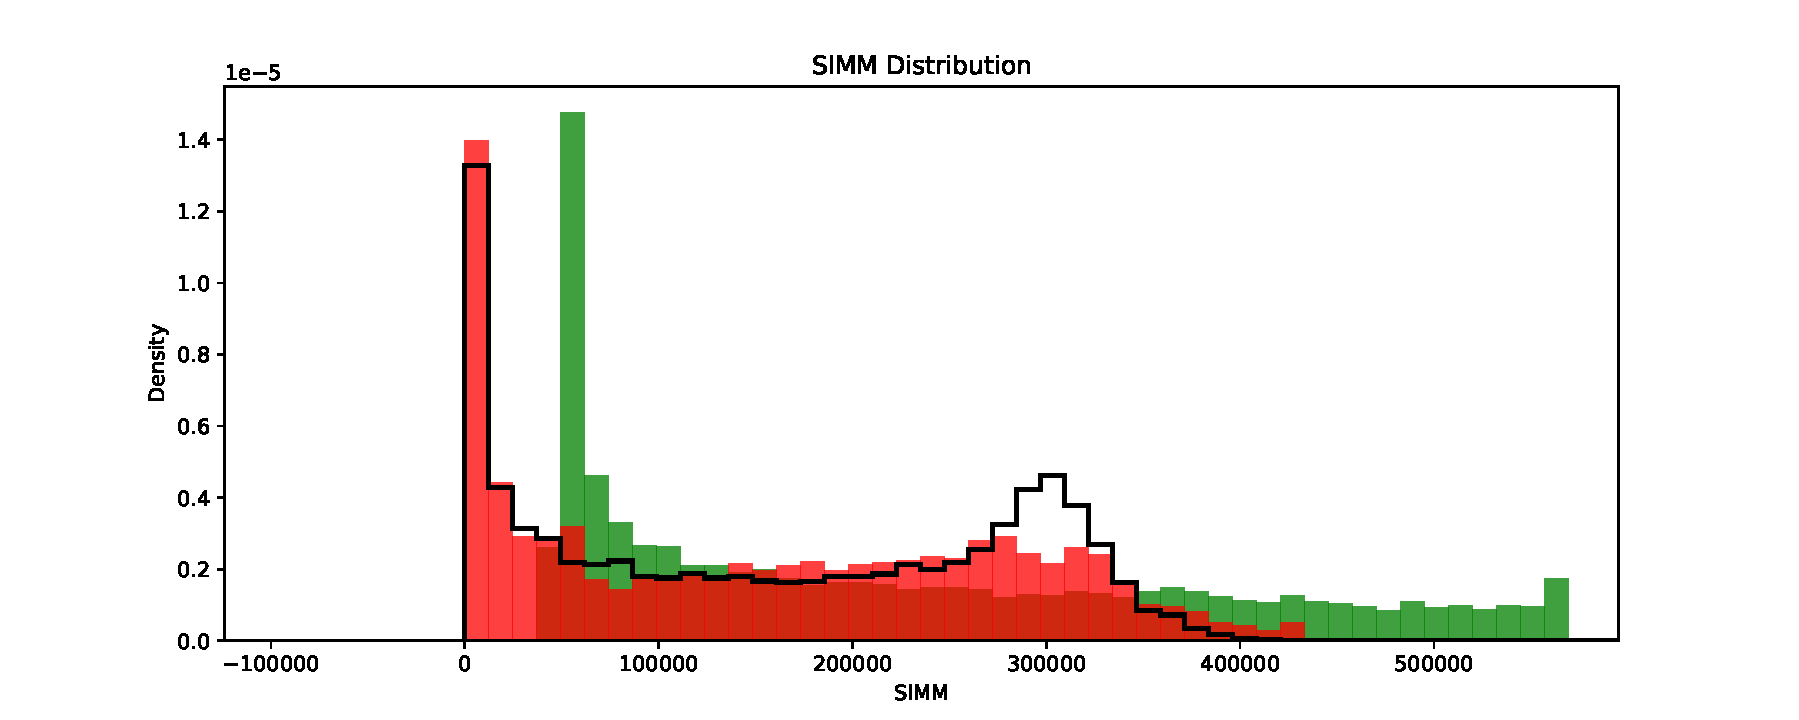
\includegraphics[width=1.0 \linewidth]{pics/mpl_simm_distribution_swaption_5y_mars_simple.pdf}
\caption{European Swaption: Dynamic SIMM distribution (red) vs benchmark II (black line) at the 5y point just before expiry.
  Top: Dynamic SIMM with polynomial regression order 4.
  Bottom: Dynamic SIMM with MARS (max terms 20) regression; also compared to scaled simple regression (green).}
\label{fig:swaptiondistribution_bench}
\end{figure}

\subsection{Bermudan Swaption}\label{sec:bermudan}

In this section we briefly investigate the case of a Bermudan Swaption in EUR, with underlying term of 5Y, first expiry in 5Y and annual expiry dates thereafter.
Typical paths are therefore as shown in figure \ref{fig:bermudanevolution}, two of which (4 and 7) drop at the 5y point indicating exercise at the first opportunity
in year 5 (high exercise value and hence SIMM), the other two continue.
Closer inspection of the benchmark simulation shows that indeed among the first 10 paths, only 2, 5, 9, 10 ``survive'' while 1, 3, 4, 6, 7 are exercised
sooner or later, so that the Dynamic SIMM evolutions are valid.
This can be seen in additional output of the Benchmark I run, where we store the differences between exercise value and continuation value
on each exercise date in the ``raw'' NPV cube.
\begin{figure}[h!]
\centering
\fig{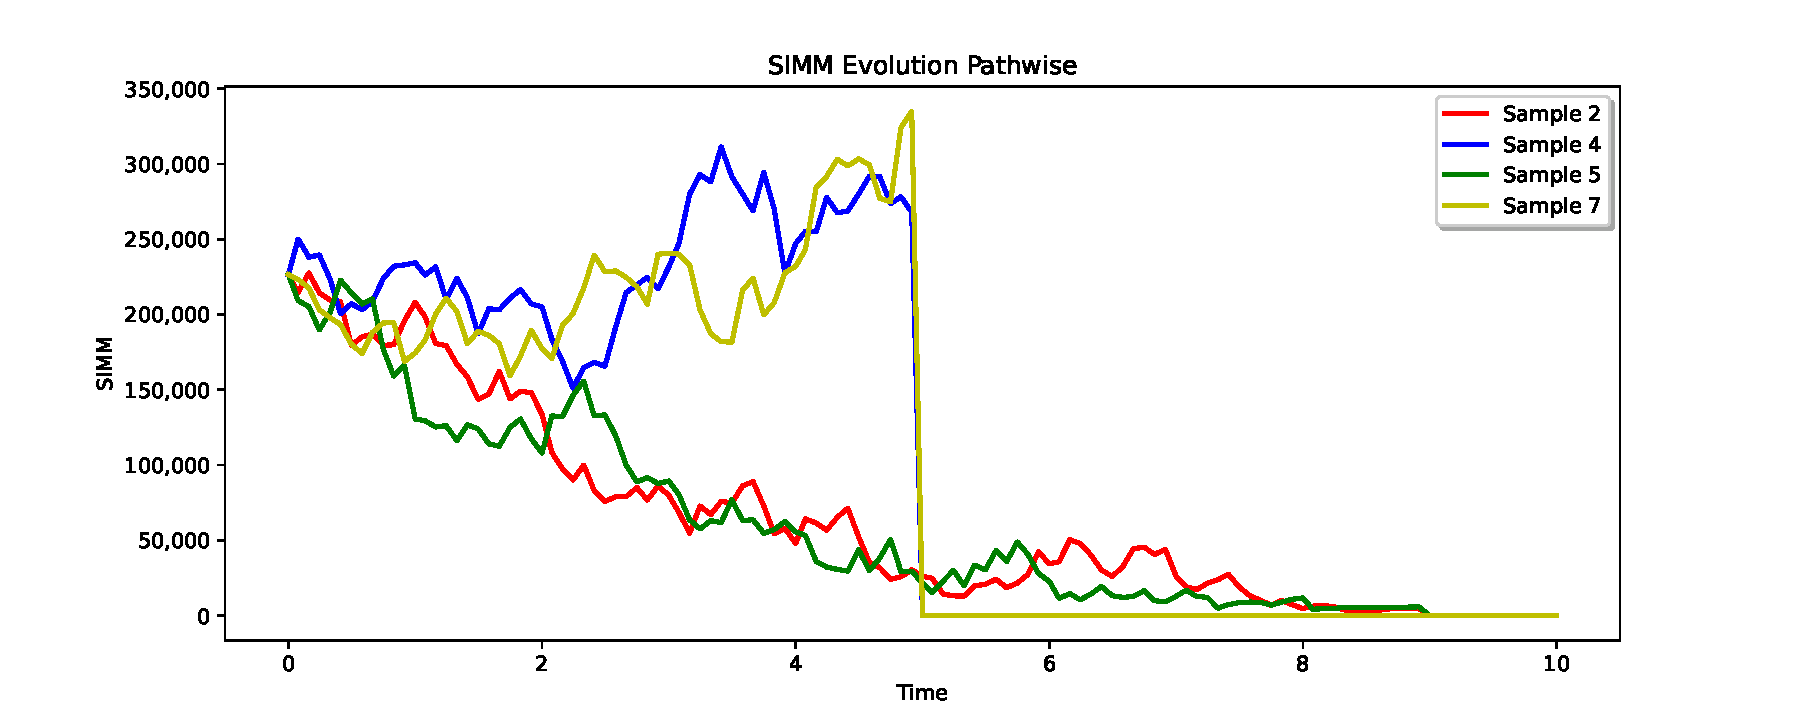
\includegraphics[width=1.0 \linewidth]{pics/fig_10_simm_evolution_pathwise_bermudan_poly.pdf}}
\caption{Bermudan Swaption with first expiry in 5Y, annual exercise dates thereafter: Selected Dynamic SIMM paths.}
\label{fig:bermudanevolution}
\end{figure}

Next, focussing on one path in each group, we compare to our benchmark I again (Benchmark II is not applicable here), see figure \ref{fig:bermudanevolution_bench}
and focus on the top row first, generated with polynomial regression.
\begin{figure}[h!]
\centering
  \begin{tabular}{cc}
\fig{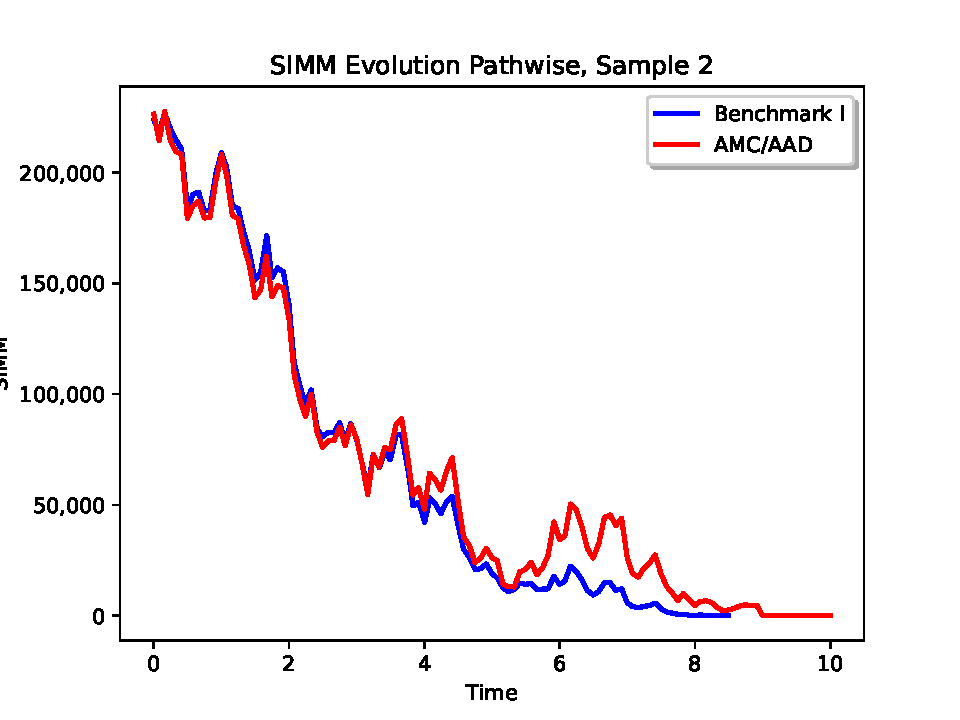
\includegraphics[width=0.5 \linewidth]{pics/fig_11a_simm_evolution_pathwise_2_0_bermudan_poly.pdf}} &
\fig{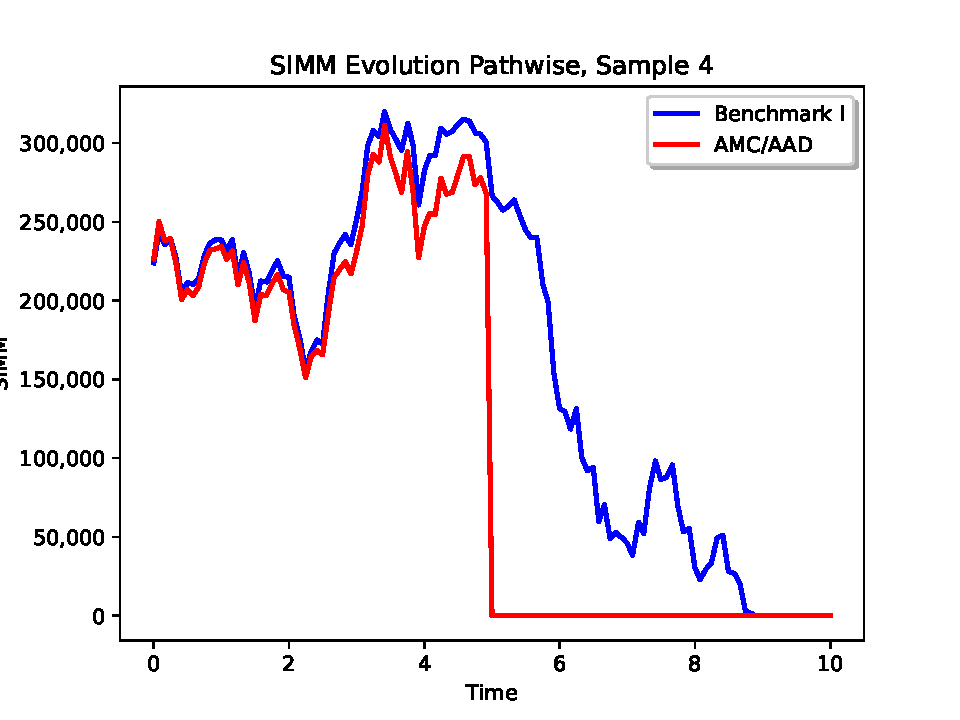
\includegraphics[width=0.5 \linewidth]{pics/fig_11b_simm_evolution_pathwise_4_0_bermudan_poly.pdf}} \\
\fig{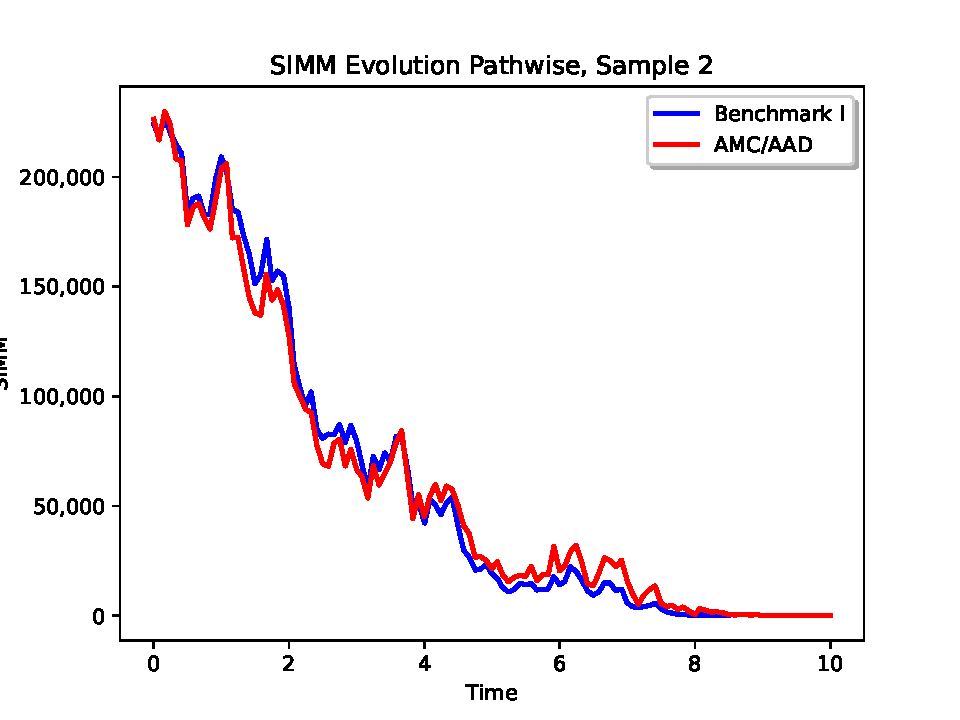
\includegraphics[width=0.5 \linewidth]{pics/fig_11c_simm_evolution_pathwise_2_0_bermudan_mars.pdf}} &
\fig{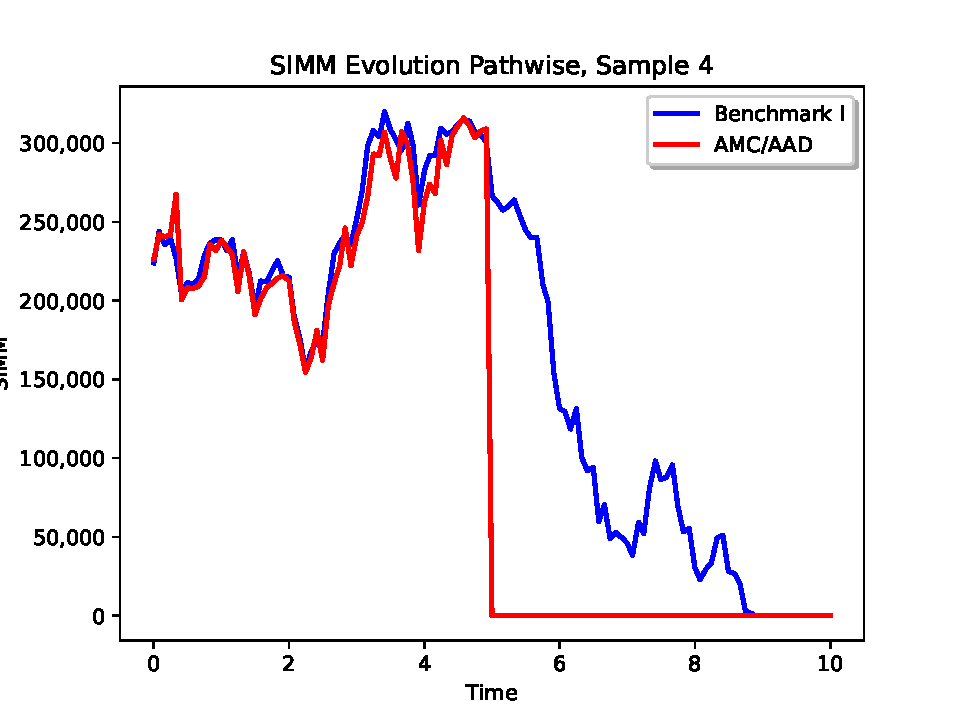
\includegraphics[width=0.5 \linewidth]{pics/fig_11d_simm_evolution_pathwise_4_0_bermudan_mars.pdf}} \\
\end{tabular}
\caption{Bermudan Swaption: Selected Dynamic SIMM paths (red) vs benchmark I (blue) with polynomial regression order 4 (top row) and MARS regression (max terms 20, bottom row). }
\label{fig:bermudanevolution_bench}
\end{figure}
On path 2 (top left), the one that does not get exercised, we see good match until first expiry and some deviation thereafter, which we attribute again to a
weakness of the polynomial regression used here. On path 4 (top right), the one that gets exercised at year 5, we see a striking discrepancy beyond year 5 at
first glance.
However, this is just because our benchmark calculation does not keep track of exercise events and rather continues as if no exercise had happened at time 5
instead of truncating -- just a weakness of the benchmarking approach which is reaching its limits with this product.
The relevant part of path 4 (up to expiry in year 5) shows a reasonable match again, with some increasing discrepancy towards expiry as we have seen in
section \ref{sec:fxoption}. So in both cases we conclude that the Dynamic SIMM evolution shown here is valid.

Finally in this section, focus on the results in the bottom row of figure \ref{fig:bermudanevolution_bench} and in
figure \ref{fig:bermudandistribution_bench}.
We see that local regression, in particular piecewise linear regression like MARS, improves the distribution match significantly.

\begin{figure}[h!]
\centering
  \begin{tabular}{cc}
\fig{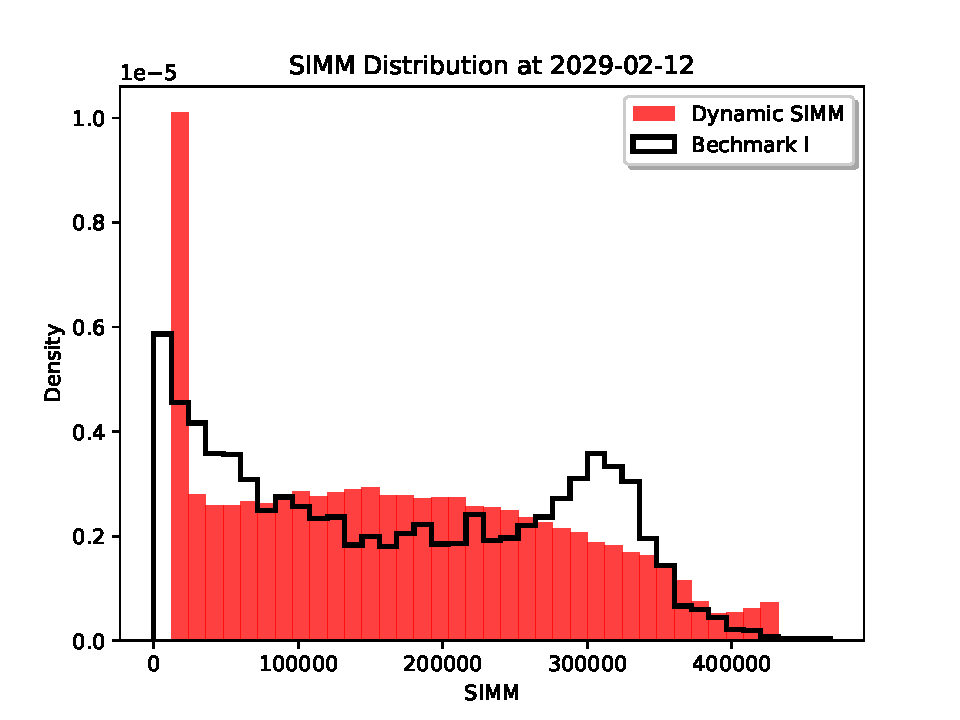
\includegraphics[width=0.5 \linewidth]{pics/fig_12a_simm_distribution_bermudan_poly4_100k.pdf}} &
\fig{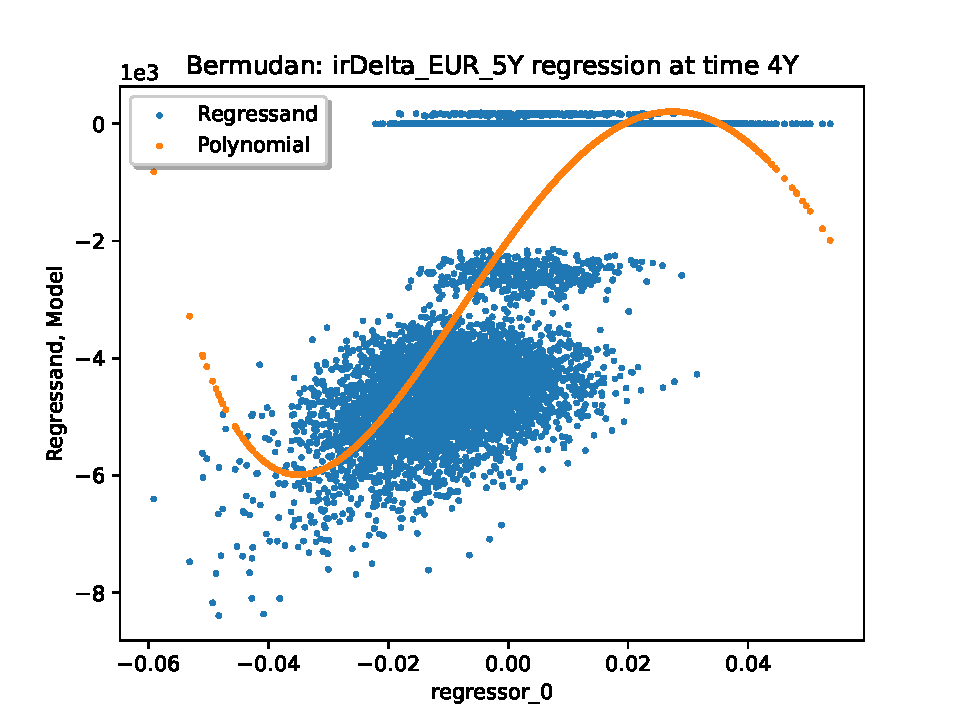
\includegraphics[width=0.5 \linewidth]{pics/fig_12b_regression_bermudan_poly4_100k_delta.pdf}} \\
\fig{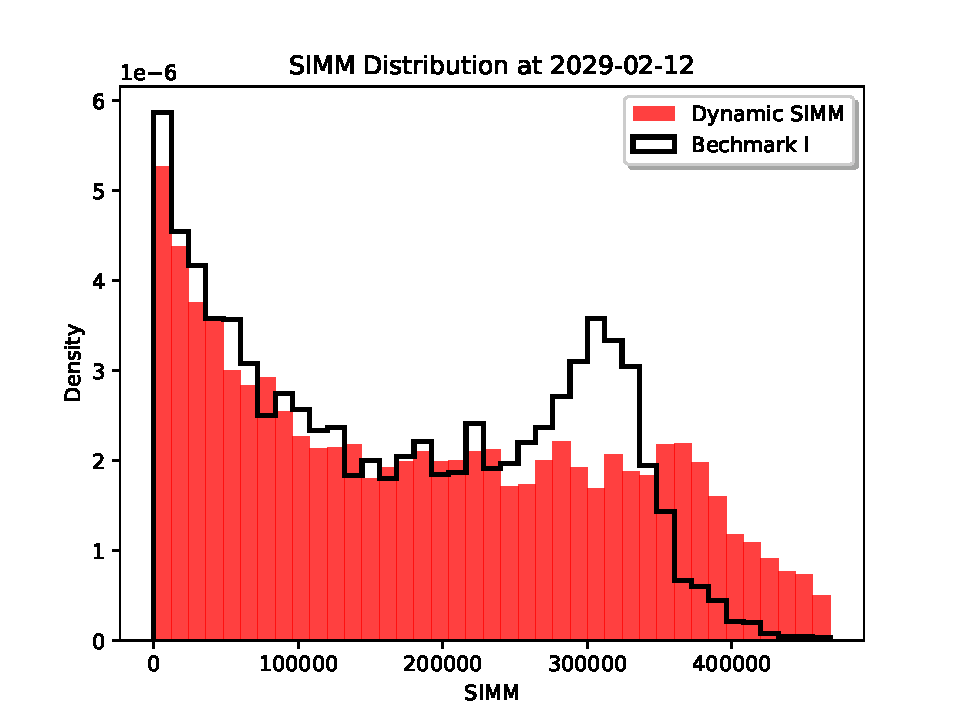
\includegraphics[width=0.5 \linewidth]{pics/fig_12c_simm_distribution_bermudan_knn100_100k.pdf}} &
\fig{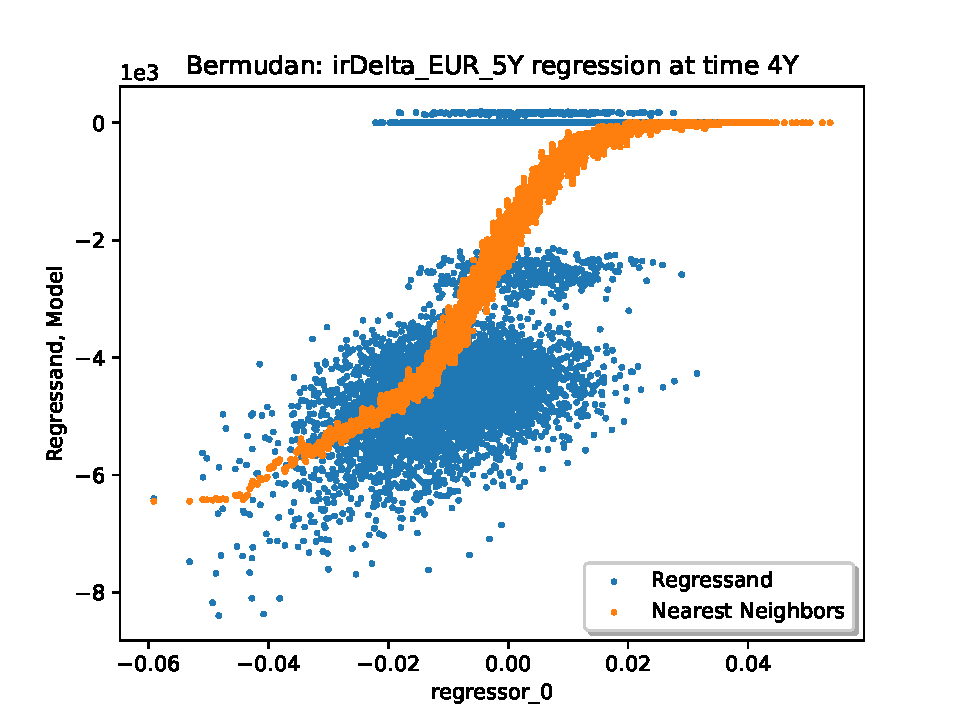
\includegraphics[width=0.5 \linewidth]{pics/fig_12d_regression_bermudan_knn100_100k_delta.pdf}} \\
\fig{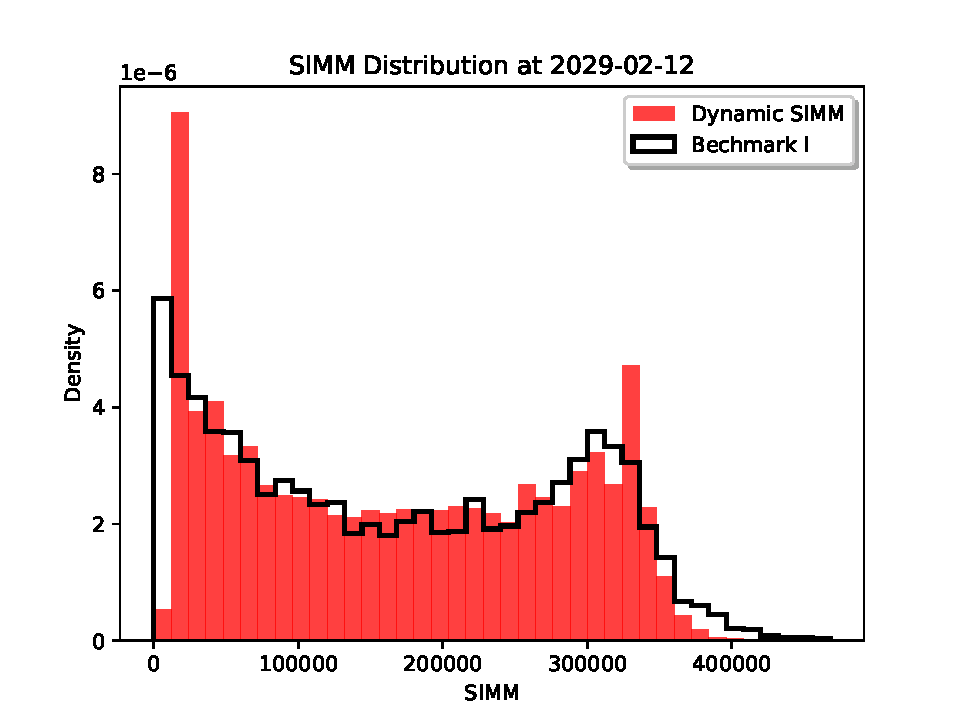
\includegraphics[width=0.5 \linewidth]{pics/fig_12e_simm_distribution_bermudan_local_100k.pdf}} &
\fig{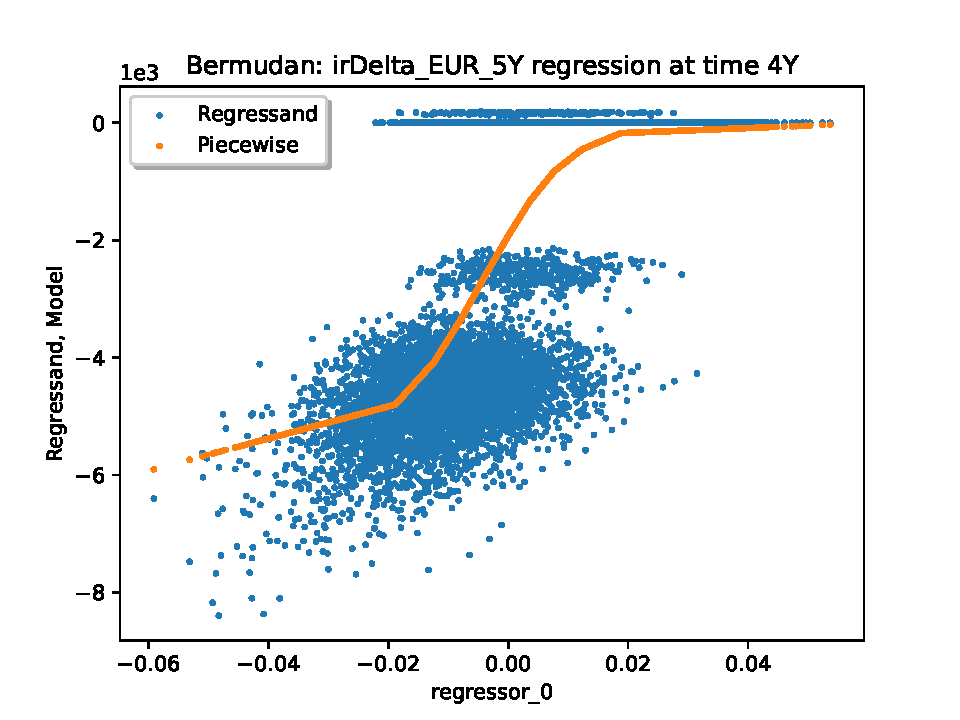
\includegraphics[width=0.5 \linewidth]{pics/fig_12f_regression_bermudan_local_100k_delta.pdf}} \\
\end{tabular}
  \caption{Bermudan Swaption: Dynamic SIMM distribution (100k samples) vs Benchmark I (5k samples) one year before the first call date and a
    typical delta regression.
    First row with 4th order polynomial regression, second row with local 100 Nearest Neighbor regression, third row with
    a combined nearest neighbour and piece-wise linear regression inspired by MARS. }
\label{fig:bermudandistribution_bench}
\end{figure}

%We will comment on performance of these methods in section \ref{sec:performance} below.
%And in section \ref{sec:applications} we shall see whether this extra detail is worth the computational effort when looking at MVA and Credit Exposure with Variation Margin and Initial Margin.

%==========================================
\section{Performance} \label{sec:performance}
%==========================================

As a performance benchmark we use the simple regression DIM model in ORE with AMC simulation.
In that model we perform valuations on a primary monthly time grid and an auxiliary close-out date grid offset from the primary grid by two weeks for
estimating NPV moves over the margin period of risk. We run 10k Monte Carlo paths and capture the computation time for the ORE process.
This is compared to the calculation time of Dynamic SIMM for the same product, primary date grid and Monte Carlo samples.
The auxiliary date grid with associated valuations is not needed here, however, complexity is significantly higher:
\begin{itemize}
\item Path-wise sensitivities are computed w.r.t. 12 yield curve tenors per currency (following the ISDA SIMM specification),
  12 IR vega expiry tenors for each currency, FX spot and 12 FX vega expiry tenors for each foreign currency;
  in our simulation setup with three currencies (EUR, GBP, USD) this means 98 sensitivities, in contrast to a single NPV in
  the benchmark calculation. These path-wise deltas and vegas are computed with AAD though, with the usual moderate overhead over NPV calculation only.
\item Large numbers of conditional expectations are computed via regressions unless all regressands are zero (e.g. beyond option expiry), see the last but one column in table \ref{tab:performance}.
\item Expected sensitivities are passed through a par conversion step on each time step and path.
\item A SIMM calculation is performed for each time step and path.
\end{itemize}
See table \ref{tab:performance} for the comparison.
In case of the simple linear products calculation time for Dynamic SIMM remains in the same ballpark as for the ``Simple DIM'' model,
the option product run times are systematically higher and vary significantly with the product, because the number of non-trivial
regressions and the regressor dimensionality varies. In one case (FX Option) we even see that the polynomial order affects run time
significantly. And MARS regression, which appears to show better results close to option expiry, shows even higher run times than the
simpler polynomial regression in general.

\begin{table}[hbt]
\scriptsize
\begin{tabular}{|l|r|rr|rr|r|r|r|}
  \hline
  \multirow{2}{*}{Product}  & \multirow{2}{*}{Simple} & \multicolumn{2}{c|}{Polynomial} & \multicolumn{2}{c|}{MARS} & \multirow{2}{*}{Steps} & \multirow{2}{*}{Regressions} & \multirow{2}{*}{Dim} \\
  & & 4 & 2 & C++ & Python & & &\\
  \hline
  \hline
  Swap          & 11  &  11  &  10  &  18  &   20 &  62  &   397  & 1 \\ 
  \hline
  FX Forward    & 11  &  56  &  52  &  40  &   57 &  62  &   918  & 3 \\ 
  \hline
  FX Option     & 11  & 171  &  68  & 138  &  200 &  62  &  4300  & 3 \\ 
  \hline
  Euro Swaption & 16  &  29  &  29  &  40  &   54 & 121  &   922  & 1 \\  
  \hline
  Berm Swaption & 17  &  42  &  40  &  54  &  108 & 121  &  2233  & 1  \\ 
  \hline
  All           & 20  & 286  & 156  & 247  &  395 & 121  &  8436  & 3  \\
  \hline
\end{tabular}
\caption{Comparison of computation times, MacBook Pro, Apple M2 Max, single-threaded. {\em Simple} stands for the Simple Regression DIM model,
  {\em Polynomial} and {\em MARS} stand for Dynamic SIMM with polynomial (order 4 and 2) resp. MARS regression. {\em Steps} is the number of time steps in the primary
  simulation grid, {\em Dim} is the regressor dimension. Row {\em All} shows run times for the portfolio of five products combined.
  The Dynamic SIMM runs with MARS use a parametrization with ``maximum degree'' 1, ``fast K'' 20, ``maximum number of terms'' 20.}
\label{tab:performance}
\end{table}

Note the two columns with MARS model runtimes in table \ref{tab:performance}: {\em Python} refers to the MARS implementation
in the {\tt py-earth2} Python package mentioned above. {\em C++} refers to the MARS/Earth implementation mentioned in section \ref{sec:sensi_regression}.
%We can thus use it, but unfortunately cannot distribute it with ORE because of uncompatible license terms.
%Providing an implementation with ORE under ORE's license terms is a subsequent task for the authors, as we see speedups of up to a factor of 2 with the C++ version
%in table \ref{tab:performance}. 

Note that for the processing of portfolios all simple products (linear, no optionality or other complexity, i.e. Swap and FX Forward above) are processed
together at the netting set level which saves regressions and helps with scalability when the portfolio contains a more significant number and fraction of
vanilla products than our test portfolio here.
Complex products are dealt with individually though, as we need to process and combine appropriate trade components as mentioned in the Models section.
Consequently, the runtime for the entire portfolio of example products (last line in table \ref{tab:performance}) is roughly the sum of runtimes for the
three Option products.

Overall we see that the price of accurate Dynamic SIMM modelling is a factor of 2-12 increase in runtime (Simple vs MARS C++) relative to the {\em Simple} model,
depending on complexity, worst case 138 vs 11 sec (FX Option case). Using MARS in Python costs up to another factor of 2.

To put the Dynamic SIMM runtimes into context, recall the runtimes of the two benchmarks we used in section \ref{sec:benchmarking}, using the FX Option
case again -- 62 time steps, {\bf 10000 paths} in 138sec with Dynamic SIMM. In that same time 
\begin{itemize}
\item Benchmark I generates 2-3 paths, speedup factor $>$1000
\item Benchmark II generates about 150-160 paths, speedup factor 60-70
\end{itemize}
Further speed optimization is possible, while sacrificing model accuracy, e.g. by computing Dynamic SIMM only on a subset of simulation dates and interpolating
path-wise between these points, or by reducing the granularity of the sensitivity grids used.
%\begin{itemize}
%\item Limit the Dynamic SIMM calculation to a subset of the simulation dates and interpolate pathwise between these points in time; for example,
%  SIMM updates on every second grid point reduces the runtime with MARS C++ for the FX Option case from 138sec to 74sec (no. of regressions from 4300 to 2198).
%\item Reduce the granularity of the sensitivity grids (using fewer points than specified by ISDA SIMM); for example, using only half of the grid points
%  reduces the runtime with MARS C++ for the FX Option case from 138sec to 114ec (no. of regressions from 4300 to 3128), i.e. with less of an effect
%\end{itemize}

\noindent
Beyond these obvious measures, more time will be invested into optimisation of the implementation, such as grouping of vanilla trades by regressor sets, avoiding
unnecessary recalculations in complex trades, to speed up the processing without loss of accuracy.
%Especially the FX Option case deserves some focus.

%==========================================
\section{Applications} \label{sec:applications}
%==========================================

Assuming that we have convinced the reader of the accuracy of the Dynamic SIMM model through the case studies in section \ref{sec:benchmarking},
and its performance in section \ref{sec:performance} that recommends its use in practice -- let us move on to applications of the model in the following.

\subsection{Margin Value Adjustment}

Given the state-dependent dynamic initial margin $\mathit{IM}(t)$, i.e. Dynamic SIMM in our OTC derivatives case, one can compute the associated funding cost
impact (MVA) as follows \cite{LSG}
$$
\MVA = \sum_{i=1}^n (f_b - s_I)\cdot \delta_i\cdot S_1(t_i)\cdot S_2(t_i) \cdot \E\left[
\mathit{IM}(t_i)\cdot D(t_i)\right]
$$
where $f_b$ is the relevant borrowing spread (relative to the cash collateral rate), $s_I$ is the spread received 
on posted initial margin, $S_{1,2}(t)$ are the cumulative survival probabilities of the two parties, $D(t)$ 
is the stochastic discount factor and $\delta_i$ is the year fraction of period $i$.
Given $\mathit{\IM}(t)$ this calculation is technically straight forward\footnote{Although the
determination of relevant spreads $f_b$ and $s_I$, in particular their term structure and projection, might be a tricky task in itself and associated with
significant uncertainty.} and also covered by ORE.
Apart from spreads $s_b$ and $s_I$, which we take as given here, it is the {\em expected discounted Initial Margin}
$$
I(t) = \E\left[\mathit{IM}(t)\cdot D(t)\right]
$$
that enters into the $\MVA$ formula.
We build upon the pathwise benchmarking of the Dynamic SIMM model above and the close match with the benchmarks seen so far.
Our focus here is now the expectation $I(t)$ and in particular the impact of regression details (polynomial vs local) on $I(t)$.

\begin{figure}[h!]
\centering
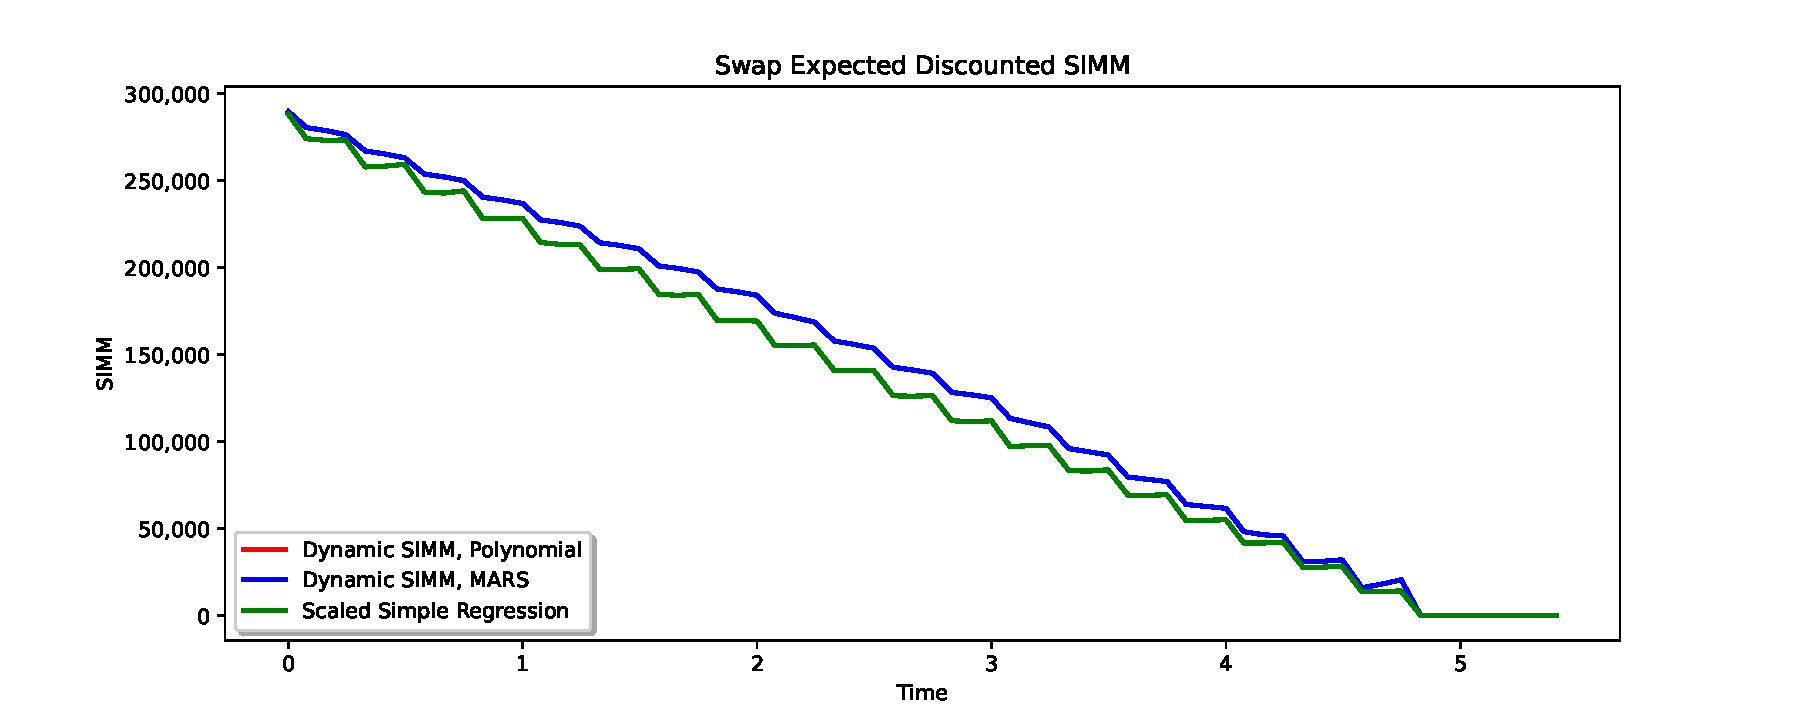
\includegraphics[width=0.9 \linewidth]{pics/mpl_simm_evolution_expected_swap_mva.pdf}
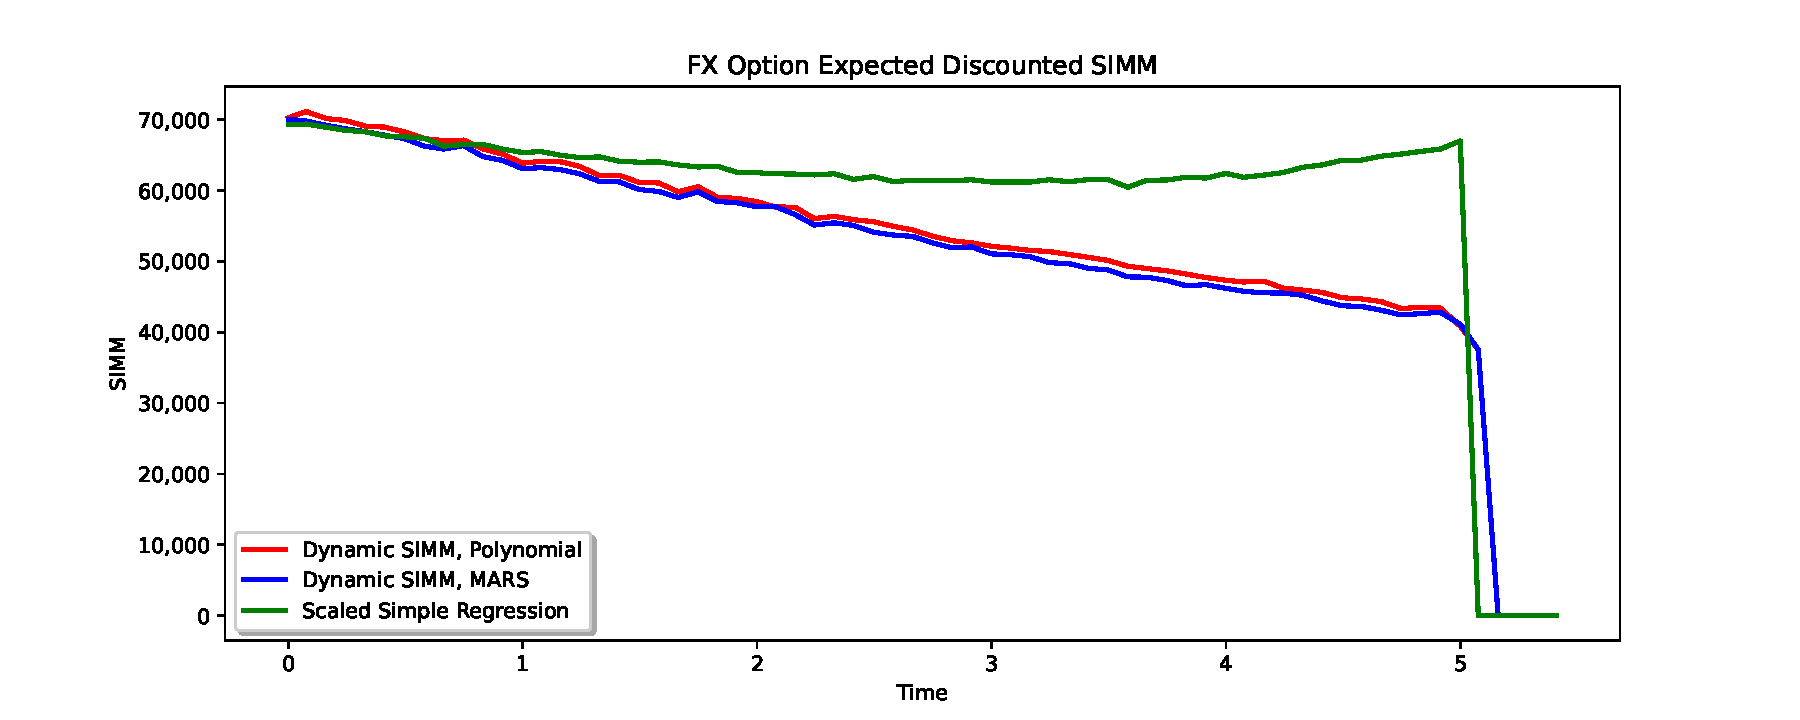
\includegraphics[width=0.9 \linewidth]{pics/mpl_simm_evolution_expected_fxoption_mva.pdf}
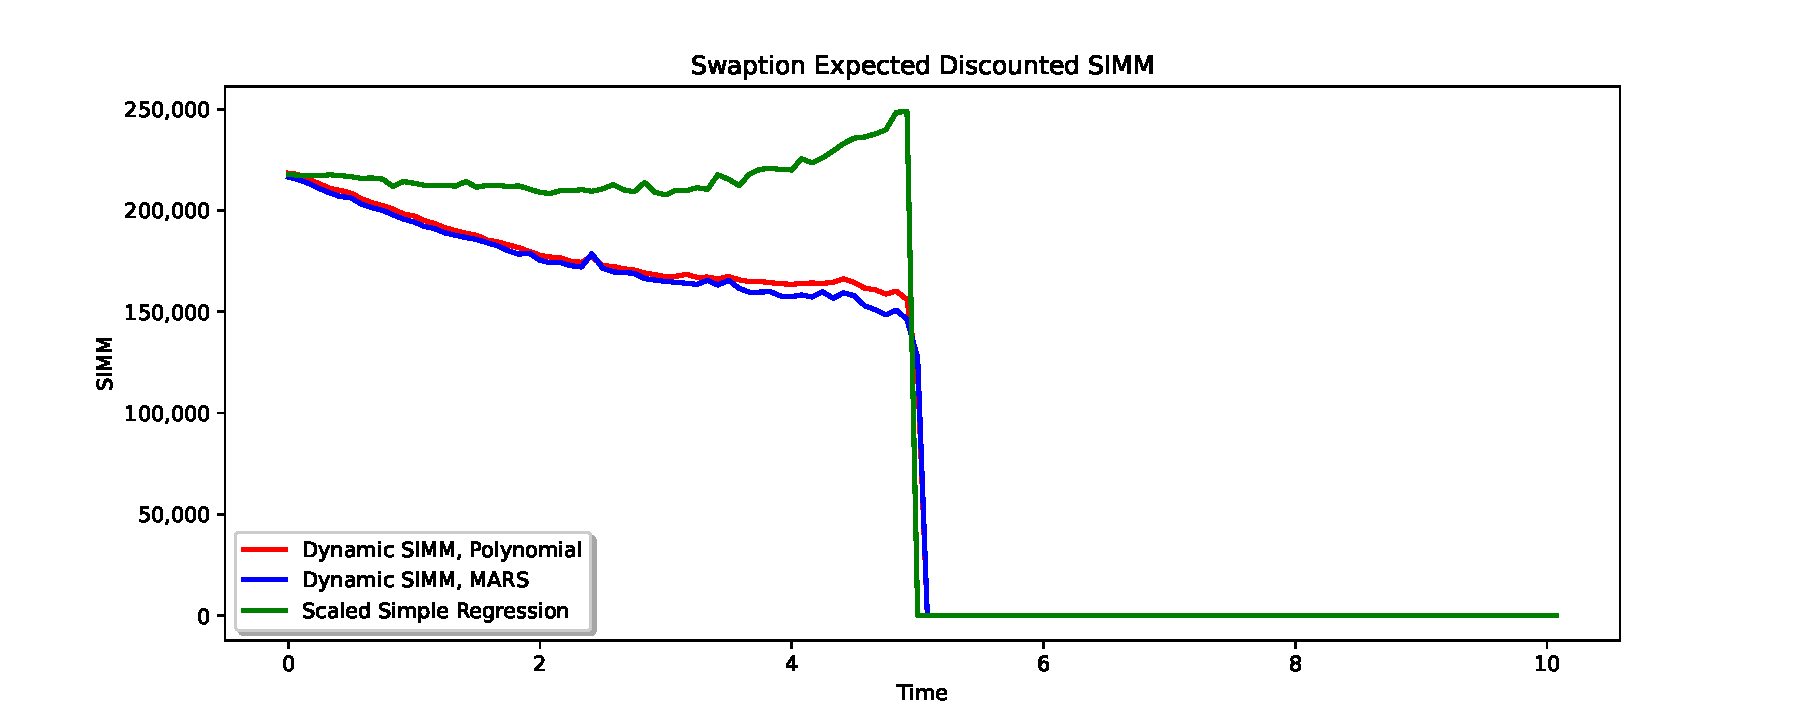
\includegraphics[width=0.9 \linewidth]{pics/mpl_simm_evolution_expected_swaption_mva.pdf}
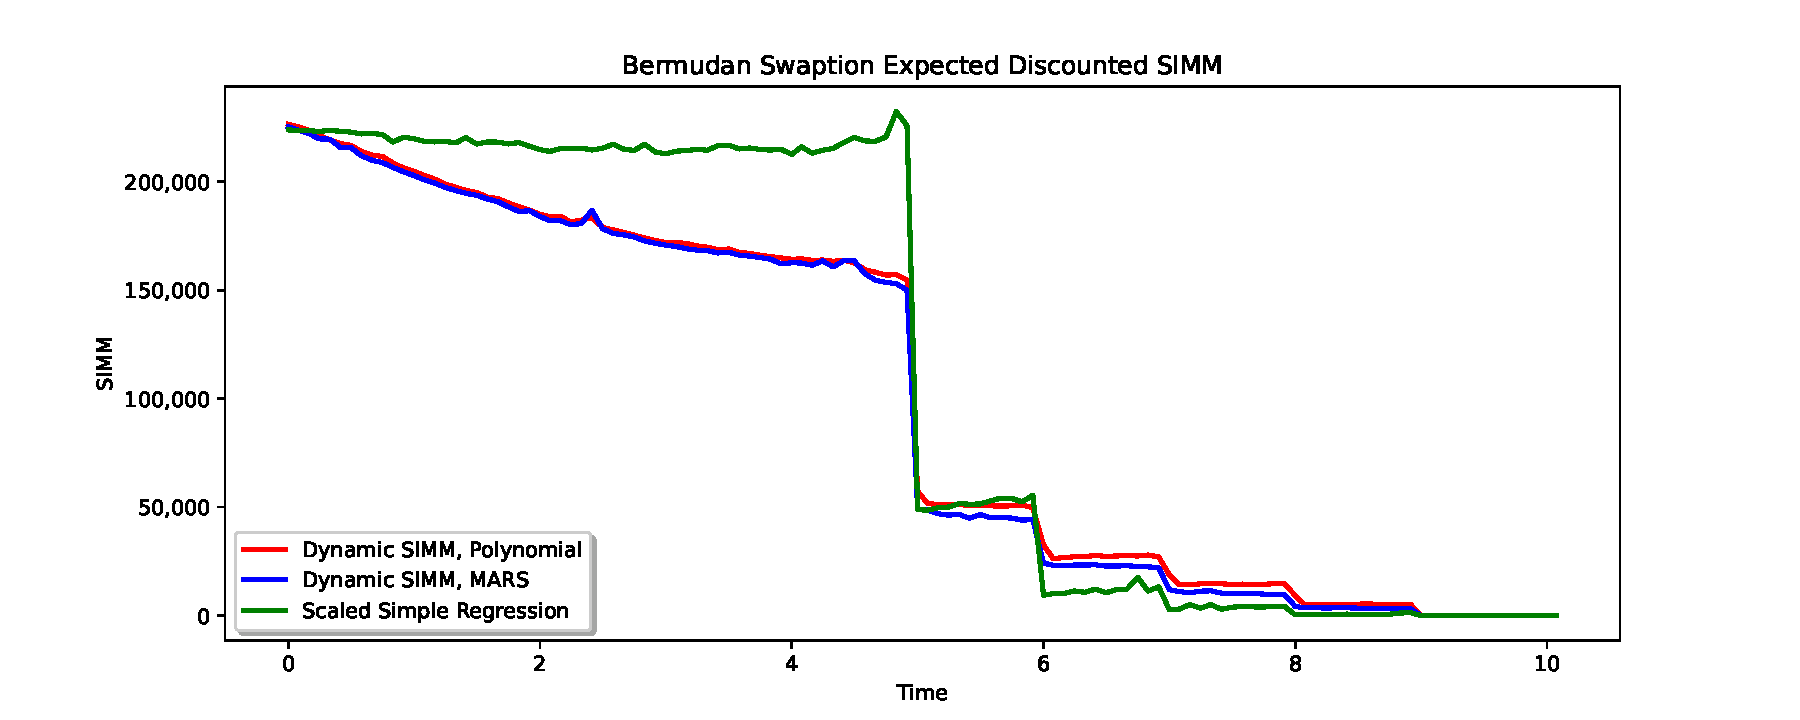
\includegraphics[width=0.9 \linewidth]{pics/mpl_simm_evolution_expected_bermudan_mva.pdf}
\caption{Expected discounted Dynamic SIMM, polyomial regression and MARS regression for the Swap, FX Option, European Swaption, Bermudan Swaption discussed above,. }
\label{fig:expected_evolutions}
\end{figure}

Figure \ref{fig:expected_evolutions} shows $I(t)$ for the single trade cases (Swap, FX Option, European Swaption, Bermudan Swaption) discussed above,
with two regression choices each (polynomial of order 4 vs MARS). For completeness we also illustrate $I(t)$ from the scaled simple regressiion model.
Note that the Dynamic SIMM based on MARS regression shows a small downwards offset compared to the polynomial regression based version: The latter
overestimates the SIMM average, consistent with the missing weight at lowest SIMM values that we have observed in the SIMM distributions in sections
\ref{sec:fxoption} and \ref{sec:swaption}.

%\clearpage

\subsection{Collateralized Exposure}

Initial Margin was introduced as additional cushion to protect against adverse developments i.e. counterparty default. So firms are keen on reflecting the
effect of IM on exposure calculations for counterparty credit risk (CCR) monitoring, CCR Capital calculations and CVA, and the expectation is that IM significantly
reduces all of the former.

Recall how CVA depends on netting set values $NPV(t)$, collateral $C(t)$ (due to VM and IM), discount factor $D(t)$, probability of default $PD$
and loss given default $LGD$, all stochastic in general:
$$
\CVA = \sum_{i} \E\left[LGD(t_i) \times \PD(t_{i-1},t_i)\times (NPV(t_i)-C(t_i))^+\times D(t_i) \right] 
$$
so that all quantities are within the expectation calculation $\E[]$. Note that only if PD and LGD are independent of the factors that drive $NPV$, $C$ and $D$, we can take
them out of the expectation and consider the simplified expected exposure
$$
 \EPE = \E\left[ (NPV(t)-C(t))^+\times D(t) \right] 
$$

The Dynamic SIMM method described in this text can be readily used in exposure calculation context, and it can be pluggged into such calculations
in ORE as a more accurate replacement for the simple regression DIM model.
If we do that in our test setup (where the model implied volatility is well below the ``internal volatility'' of the SIMM model), and compute the simplified $\EPE$,
then we see a small residual exposure -- after applying VM and IM pathwise -- within the Monte Carlo noise order of magnitude. If we shock the market, doubling the
Euro Swaption volatiltiy level, then we see the resulting exposures as shown in figure \ref{fig:exposure} for the Bermudan Swaption case. Note the differences in
vertical scale of the exposure plots.
\begin{figure}[hbt!]
\centering
\begin{tabular}{cc}
  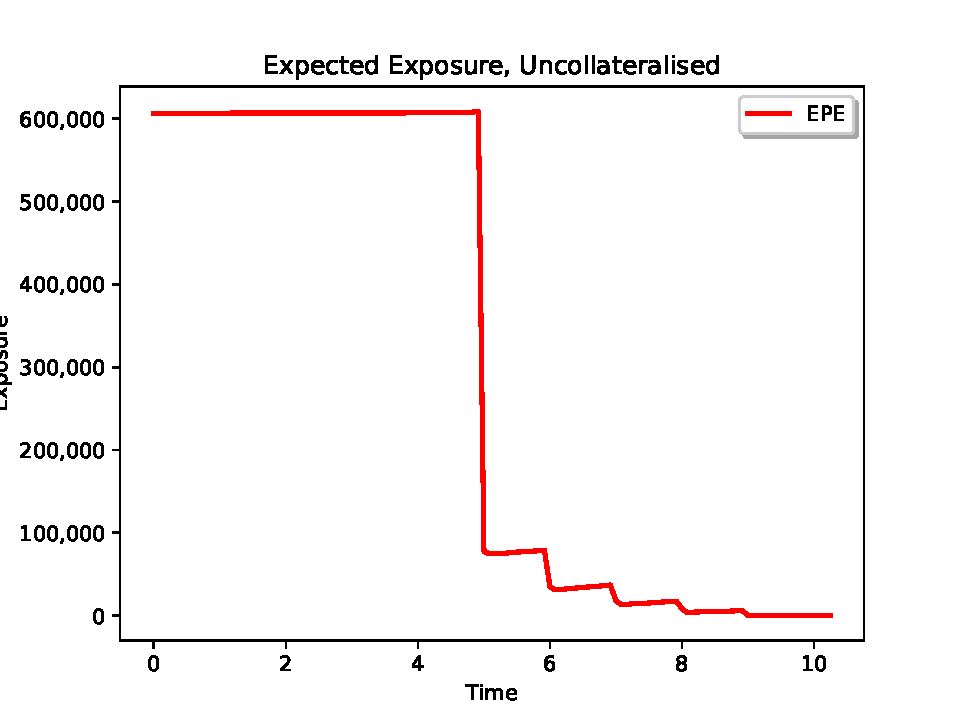
\includegraphics[width=0.5 \linewidth]{pics/mpl_exposure_bermudan_poly_none.pdf} &
  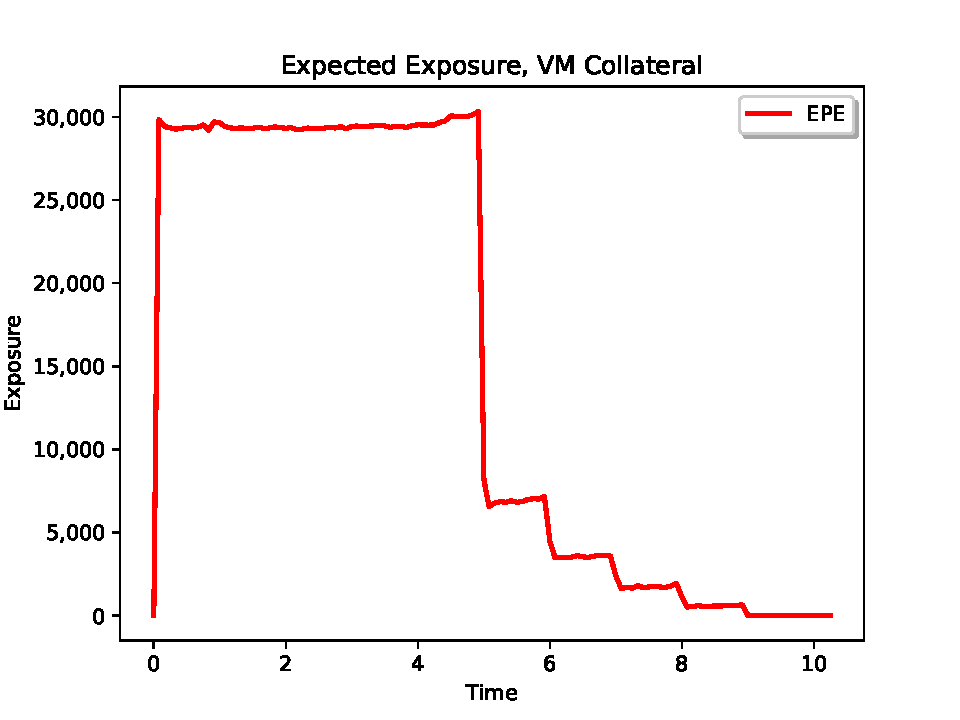
\includegraphics[width=0.5 \linewidth]{pics/mpl_exposure_bermudan_poly_vm.pdf} \\
  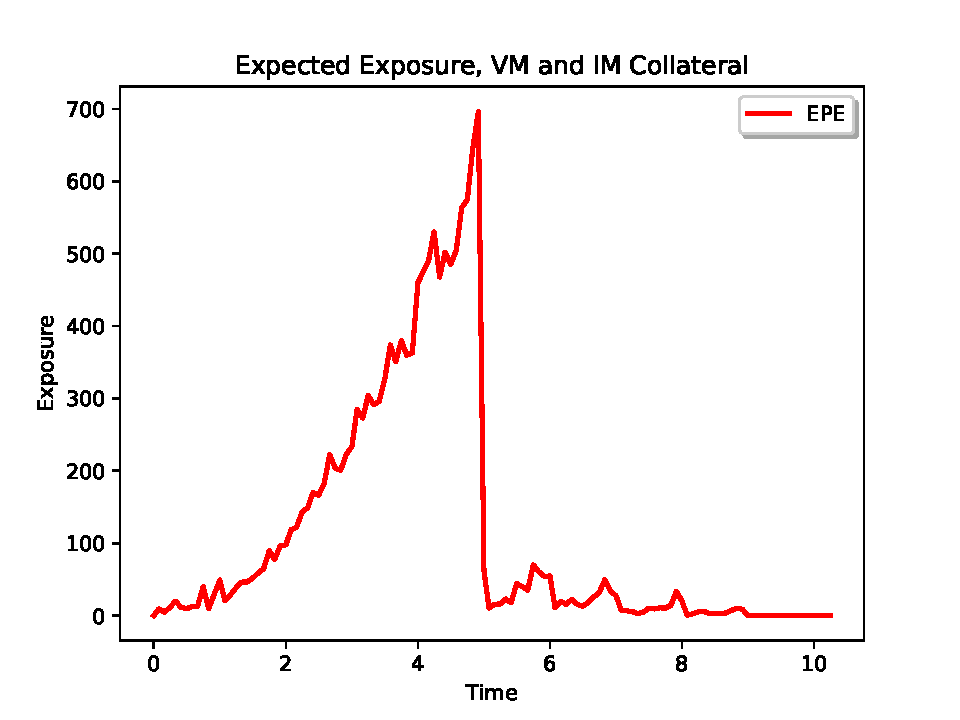
\includegraphics[width=0.5 \linewidth]{pics/mpl_exposure_bermudan_poly_im.pdf} & 
  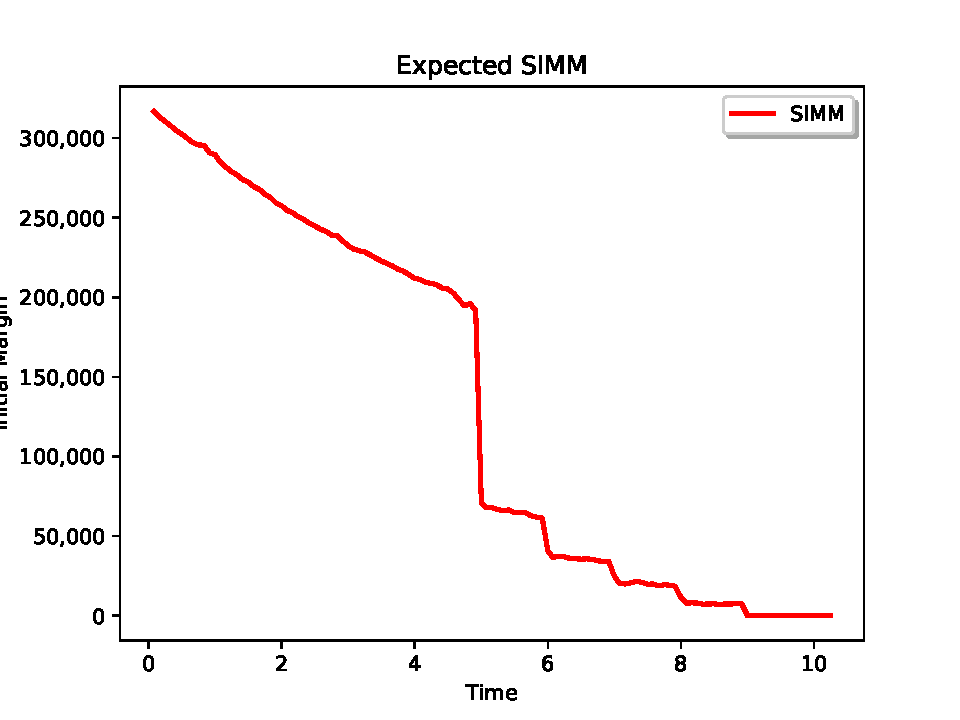
\includegraphics[width=0.5 \linewidth]{pics/mpl_dim_evolution_poly.pdf} \\
\end{tabular}
\caption{Expected exposure for the Bermudan Swaption case, uncollateralized (top left), with VM only and zero thresholds/minimum transfer amount (top right),
  with VM and IM using the Dynamic SIMM model (bottom left). The expected Initial Margin evolution is also shown (bottom right).
  The market is stressed, replacing the 75bp EUR Swaption volatility level with 150bp. We used 100k Monte Carlo paths to improve statistics for the exposure after VM and IM.
  % Reversion speed 0
  % Polynomial regression order 6
}
\label{fig:exposure}
\end{figure}

Finally, as we have seen with the Archaegos case, the naive assumption of independence between stochastic default probability and exposure
can be misleading, and one should also consider dependence e.g. as in \cite{arnsdorf_2023}, \cite{pykhtin_2024}, or \cite{anfuso_2024, anfuso_2025} -- at least
as a stress test -- where one suspects dealing with leveraged counterparties.

%==========================================
\section{Conclusion} \label{sec:conclusions}
%==========================================

%The further investigation of local regression methods that can be applied reliably through the life of a portfolio, with some focus on MARS,
%is work in progress. Note that the local regression methods explored so far come with additional computational cost, compared to basic polynomial regression.
%We will provide some performance indications in section \ref{sec:performance} below. \\

The Dynamic SIMM method, as implemented in ORE, provides accurate SIMM under Monte Carlo simulation, covering ``linear'' products, Options and Exotics,
for a moderate increase of computational effort. We have observed factors 2-12 in computation time compared to the Simple DIM method,
for the products investigated in this paper. Our benchmarking has shown that the choice of sensitivity regression method embedded in the American Monte Carlo simulation 
affects the quality of simulated sensitivities noticeably. We have identified one promising local regression method so far ({\em Multivariate Adaptive Regression
Splines (MARS)} that improves the match with benchmark results, with little additional computational effort compared to global polynomial regression.
Dynamic SIMM in ORE uses {\em Adjoint Algorithmic Differentiation (AAD)} to compute path-wise sensitivities under Monte Carlo scenarios efficiently. The
implementation in ORE avoids the usual {\em Operator Overloading} approach (across the entire library), but demonstrates the use of an explicit
{\em Computation Graph} that allows activating AAD in specific parts of the library and without recompiling the entire project. \\

\noindent
Future work will address current limitations of the implementation
\begin{itemize}
\item extending the risk class scope beyond IR/FX;
\item extending the exotic product scope with additional regressors and appropriate product decompositions;
\item distinguishing ISDA SIMM to call and to post;
\item further optimising performance, avoiding repeated calculations of regressions that can be cached;
\item adding an implementation of the Multivariate Adaptive Regression Spline (MARS) method in C++ to distribute with ORE,
  also as a basis for modifications as demonstrated in Figure \ref{fig:bermudandistribution_bench}, bottom row, in the one-dimensional case
\item researching the impact and performance of further local regression methods
\end{itemize}

We hope -- with the help of the open-source implementation in ORE -- to see the Dynamic SIMM method applied more broadly, in model validation if not production
applications, in providing accurate training data for machine learning approaches to exposure simulation and MVA with Dynamic Initial Margin
\cite{aryan_2020,villarino_2024}, and to motivate community contribution to the method's further investigation and development.
In this context, the newly introduced integration of ORE with Python (i.e. facilitating ORE calls from C++ into Python) makes it particularly easy to explore
alternative methods for the calculation of conditional expectations that are so central to the method, since these calculations can now be redirected
to any user provided python code leveraging the vast supply of machine learning libraries in this space.

\section{Use of artificial intelligence}

No use of artificial intelligence tools has been made in the generation of results presented here, nor in writing the text of this article.

\begin{appendix}


  
\section{List of Abbreviations}

\begin{table}[h!]
	\centering
	\begin{tabular}{ | m{10cm} | m{1.4cm}| } 
		\hline
		\multicolumn{2}{|c|}{\textbf{List of abbreviations}} \\
		\hline
		Net Present Value & NPV \\
                \hline
                Variation Margin & VM \\
		\hline
		Initial Margin & IM \\
		\hline
		Margin Period of Risk & MPOR \\
		\hline
		Standard Initial Margin Model & SIMM  \\ 
		\hline
		Common Risk Interchange Format & CRIF  \\ 
		\hline
		Dynamic Initial Margin & DIM  \\ 
		\hline
		Value at Risk & VaR  \\ 
		\hline
		Credit Support Annex & CSA  \\ 
		\hline
		Credit Valuation Adjustment & CVA  \\ 
		\hline
		Margin Valuation Adjustment & MVA  \\ 
		\hline
		Basel Committee on Banking and Supervision & BCBS  \\ 
		\hline
		International Organisation of Securities Commissions & IOSCO  \\ 
		\hline
		International Swaps and Derivatives Association & ISDA  \\ 
		\hline
                ORE's Cross Asset Market Simulation Model & CAM \\
                \hline
                Linear Gauss Markov & LGM \\
                \hline
                One-Factor Linear Gauss Markov & LGM1F \\
                \hline
                Geometric Brownian Motion & GBM \\
                \hline
                American Monte Carlo & AMC \\
                \hline
                Computation Graph & CG \\
                \hline
                Adjoint Algorithmic Differentiation & AAD \\
                \hline
                Interest Rate & IR \\
                \hline
                Foreign Exchange & FX \\
                \hline
                Multivariate Adaptive Regression Splines & MARS \\
                \hline
	\end{tabular}
	\caption{List of the abbreviations introduced in the main text.}
\end{table}


%\section{Biographies}
%Peter Caspers is Lead Quant Developer at LSEG Post Trade Solutions with over 25 years experience in various quantitative roles. He is regular contributor to QuantLib and one of the core developers of Open Source Risk Engine (ORE). He holds a degree in mathematics from the University of Dortmund. \\

%Roland Lichters is Co-Head of Quantitative Services at Acadia, now LSEG Post Trade, former co-founder and CTO of Quaternion Risk Management, following 15 years in financial institutions with leading roles in IT and Risk. He has driven the continuous release of Open Source Risk Engine (ORE) since 2016. Roland holds a PhD in Physics and lectures part time at Northeastern University, Boston. He is co-author of the book 'Modern Derivatives Pricing and Credit Exposure Analysis'.


\end{appendix}

\addcontentsline{toc}{section}{Bibliography}
\typeout{[Bibliography]}

\begin{thebibliography}{10}

% Ref 1  
\bibitem{IMBIS}
  Basel Committee on Banking Supervision,
  (2015),
  ``Margin requirements for non-centrally cleared derivatives'',
  available online at \url{www.bis.org/publ/bcbs261.pdf}.

% Ref 2  
\bibitem{ISDASIMM}
  International Swaps and Derivatives Association (ISDA),
  (2025),
  ``ISDA SIMM\texttrademark Methodology, version 2.7'',
  available online at \url{https://www.isda.org/a/f2RgE/ISDA-SIMM_v2.82506_PUBLIC.pdf}.

% Ref 3
\bibitem{PykhtinDIM}
  Andersen, L., Pykhtin, M., Sokol, A.,
  (May 2017),
  ``Does initial margin eliminate counterparty risk?'',
  Risk,
  %``Credit Exposure in the Presence of Initial Margin'',
  working paper available online at \url{https://ssrn.com/abstract=2806156}.

% Ref 4  
\bibitem{green2014im}
  Green, A., Kenyon, C.,
  (April 2015),
  ``MVA by replication and regression'',
  Risk, 
  working paper available online at \url{https://ssrn.com/abstract=2432281}.

% Ref 5  
\bibitem{FabrizioAnfusoDIM}
  Anfuso, F., Aziz, D., Giltinan, P., Loukopoulos, K.,
  (May 2017),
  ``A sound modelling and backtesting framework for forecasting initial margin requirements'',
  Risk.

% Ref 6
\bibitem{PykhtinDIM-2}
  Andersen, L., Pykhtin, M., Sokol, A., ref. 3 above

% Ref 7  
\bibitem{FabrizioAnfusoDIM-2}
  Anfuso, F., Aziz, D., Giltinan, P., Loukopoulos, K., ref. 5 above

% Ref 8
\bibitem{Caspers2017}
  Caspers, P., Giltinan, P., Lichters, R., Nowaczyk, N.,
  (2017),
  ``Forecasting initial margin requirements: A model evaluation'', 
  Journal of Risk Management in Financial Institutions, Vol. 10, 4, pp. 365-394,
  working paper available online at \url{https://ssrn.com/abstract=2911167}.

% Ref 9
\bibitem{fries_2017}
  Fries,C.,
  (2017),
  ``Stochastic Automatic Differentiation: Automatic Differentiation for Monte-Carlo Simulations'',
  available online at \url{https://ssrn.com/abstract=2995695};\\
  ``Automatic Backward Differentiation for American Monte-Carlo Algorithms - AAD for Conditional Expectations and Indicator Functions'',
  available online at \url{https://ssrn.com/abstract=3000822};\\
  ``Fast Stochastic Forward Sensitivities in Monte-Carlo Simulations Using Stochastic Automatic Differentiation (with Applications to Initial Margin Valuation Adjustments (MVA))'',
  available online at \url{https://ssrn.com/abstract=3018165}.

% Ref 10
\bibitem{caspers_2018}
  Caspers, P., Lichters, R.,
  (2018),
  ``Initial Margin Forecast - Bermudan Swaption Methodology and Case Study'',
  available online at \url{https://ssrn.com/abstract=3132008}.
  
% Ref 11
\bibitem{antonov_2017}
  Antonov, A., Issakov, S., McClelland, A.,
  (September 2018),
  ``Efficient SIMM-MVA Calculations for Callable Exotics'',
  Risk,
  working paper available online at \url{https://ssrn.com/abstract=3040061}.
  
% Ref 12
\bibitem{jain_2017}
  Jain, S., Laitao, A., Oosterlee, C.,
  (April 2019),
  ``Rolling Adjoints: fast Greeks along Monte Carlo scenarios for early-exercise options'',
  Journal of Computational Science, Vol. 33, 
  working paper available online at \url{https://ssrn.com/abstract=3093846}.

%\bibitem{savine_cg_1} A:~Savine,
%  Computation Graphs for AAD and Machine Learning Part I: \\
%  Introduction to Computation Graphs and Automatic Differentiation, 2019,\\
%  \url{https://www.researchgate.net/publication/337201082_Computation_Graphs_for_AAD_and_Machine_Learning_Part_I_Introduction_to_Computation_Graphs_and_Automatic_Differentiation}

%\bibitem{savine_cg_2} A:~Savine,
%  Computation Graphs for AAD and Machine Learning Part II: \\
%  Adjoint Differentiation and AAD, 2020\\
%  \url{https://www.researchgate.net/publication/338662793_Computation_Graphs_for_AAD_and_Machine_Learning_Part_II_Adjoint_Differentiation_and_AAD}

%\bibitem{savine_cg_3} A:~Savine,
%  Computation Graphs for AAD and Machine Learning Part III: \\
%  Application to Derivatives Risk Sensitivities, 2020, \\
%  \url{https://www.researchgate.net/publication/340126636_Computation_Graphs_for_AAD_and_Machine_Learning_Part_III_Application_to_Derivatives_Risk_Sensitivities}

%\bibitem{savine_book_1}
%  A.~Savine and L.~Andersen.
%  Modern Computational Finance: AAD and Parallel Simulations,
%  Wiley, 2018

%\bibitem{savine_book_2}
%  A.~Savine and J.~Andreasen.
%  Modern Computational Finance: Scripting for Derivatives and xVA
%  Wiley, 2021

%\bibitem{capriotti_2023}
%  L.~Capriotti, M.~Giles.
%  \newblock {15 Years of Adjoint Algorithmic Differentiation in Finance}.
%  \newblock {Available online at {https://ssrn.com/abstract=4588939}, 2023.}

% Ref 13
\bibitem{lakhani_2021}
  Lakhani, A., Zhang, A.,
  (October 2021),
  ``Efficient ISDA Initial Margin Calculations using Least Squares Monte-Carlo'',
  available online at \url{https://arxiv.org/pdf/2110.13296}.
  
% Ref 14
\bibitem{zeron_2021}
  Zeron, M., Ruiz, I.,
  (April 2021),
  ``Tensoring Dynamic Sensitivities and Dynamic Initial Margin'',
  Risk.

% Ref 15
\bibitem{aryan_2020}
  Aryan, A., Cowan, A.,
  (July 2020),
  ``Deep MVA: Deep Learning for Margin Valuation Adjustment of Callable Products'',
  working paper available online at \url{https://ssrn.com/abstract=3634059}.

% Ref 16
\bibitem{villarino_2024}
  Vilarino, J., Laitao, A.,
  (July 2024),
  ``On Deep Learning for computing the Dynamic Initial Margin and Margin Value Adjustment'',
  working paper available online at \url{https://doi.org/10.48550/arXiv.2407.16435}.

% Ref 17
\bibitem{ORE}
  Open Source Risk Engine (ORE),
  ``A free/open-source platform for risk analytics and XVA'' \\
  Project site: \url{https://opensourcerisk.org} \\
  Source code: \url{https://github.com/opensourcerisk/engine} \\
  Documentation: \url{https://github.com/opensourcerisk/engine/tree/master/Docs} \\
  Introduction: \url{https://www.youtube.com/@oreacademy}

% Ref 18
\bibitem{ORE-2}
  ORE documentation, ref. 17 above.

% Ref 19
\bibitem{fries_2017-2}
  Fries, C., ref. 9 above.

% Ref 20
\bibitem{ORE-3}
  ORE documentation, ref. 17 above.

% Ref 21
\bibitem{ORE-4}
  ORE documentation, ref. 17 above.

% Ref 22
\bibitem{piterbarg_deltas_callable_libor_exotics}
  Piterbarg, V.,
  (January 2004),
  ``Computing Deltas of Callable Libor Exotics in Forward Libor Models'',
  Journal of Computational Finance 7(3),
  working paper available online at: \url{https://ssrn.com/abstract=396180}.

% Ref 23 
\bibitem{MARS}
  Friedman, J.H.,
  (1991),
  ``Multivariate Adaptive Regression Splines'',
  The Annals of Statistics, 19 (1).

% Ref 24
\bibitem{mars-rojas}
  Rojas, C.,
  (2017),
  ``An Implementation of MARS in C++ and C\#'',
  available online at \url{https://github.com/cesar-rojas/mars}

% Ref 25
\bibitem{caspers2017_2}
  Caspers, P., Giltinan, P., Lichters, R., Nowaczyk, N., ref. 8 above.

%\bibitem{mars-r}
%  Multivariate Adaptive Regression Splines in R,
%  available online at \url{https://cran.r-project.org/web/packages/earth}

\bibitem{LSG}
  Lichters, R., Stamm, R., Gallagher, D.,
  (2015),
  ``Modern Derivatives Pricing and Credit Exposure Analysis. Theory and Practice of CSA and XVA Pricing, Exposure Simulation and Backtesting'',
  Palgrave Macmillan.

\bibitem{arnsdorf_2023}
  Arnsdorf, M.,
  (January 2023)
  ``Leveraged wrong-way risk'',
  Risk,
  working paper available online at \url{https://ssrn.com/abstract=4340426}.
  
%\bibitem{anfuso_2023}
%  Anfuso, F.,
%  (January 2023),
%  ``Collateralised exposure modelling: bridging the gap risk.''
%  Risk,
%  working paper availabel online at \url{https://ssrn.com/abstract=4098381}.

\bibitem{pykhtin_2024}
  Pykhtin, M.,
  (June 2024)
  ``Weighting for Leverage'',
  Risk,
  working paper available online at \url{https://ssrn.com/abstract=4691135}.

\bibitem{anfuso_2024}
  Anfuso, F.,
  (July 2024),
  ``Bridging the gap risk reloaded: a comprehensive methodology for wrong way risk and leveraged exposures'',
  Risk,
  working paper available online at \url{https://ssrn.com/abstract=4456371}.

\bibitem{anfuso_2025}
  Anfuso, F., Karyampas, D.,
  (April 2024),
  ``The WWR in the tail: a Monte Carlo framework for CCR stress testing'',
  Risk,
  working paper available online at \url{https://ssrn.com/abstract=5074421}.

\end{thebibliography}

\end{document}

